
%% cross-references, and citations.

\documentclass[11pt]{book}
\usepackage{Wiley-AuthoringTemplate}
\usepackage[sectionbib,authoryear]{natbib}
% for name-date citation comment the below line
%\usepackage[sectionbib,numbers]{natbib}% for numbered citation comment the above line

%%********************************************************************%%
%%       How many levels of section head would you like numbered?     %%
%% 0= no section numbers, 1= section, 2= subsection, 3= subsubsection %%
\setcounter{secnumdepth}{3}
%%********************************************************************%%
%%**********************************************************************%%
%%     How many levels of section head would you like to appear in the  %%
%%				Table of Contents?			%%
%% 0= chapter, 1= section, 2= subsection, 3= subsubsection titles.	%%
\setcounter{tocdepth}{2}
%%**********************************************************************%%

%\includeonly{ch01}
\makeindex
\usepackage{pdfpages}
\usepackage{hyperref}
\newcommand\Emph{\textbf}
\newcommand\p{^{\prime}}
\newcommand\pp{^{\prime\prime}}
\newcommand{\lapl}[1]{\mathscr{L}\{#1\}}
\newcommand{\X}{\mathbb{X}}
\newcommand{\dX}{\dot{\mathbb{X}}}
\newcommand{\fX}{\bar{\text{\b{X}}}}
%\includeonly{week10/Wednesday}

\begin{document}

\frontmatter

\booktitle{A First Course \\ In \\
Ordinary differential equations}
 
\subtitle{MAT2002 Notebook}

\AuAff{Prof. Weiming Ni\\ The Chinese University of Hongkong, Shenzhen}


\halftitlepage
\titlepage  



\tableofcontents


\acknowledgments
This book is from the MAT2002 in spring semester, 2019. In addition, some material is cited from {\it Differential Equations and Their Applications $4^{th}$} by Martin Braun.
\authorinitials{CUHK(SZ)}  


\mainmatter
\setcounter{page}{1}

\chapter{Week8}

\section{Monday}\index{Monday_lecture}
\subsection{Euler's Equation}
Recall previous knowledge,
\[t^2y\pp+\alpha ty\p+\beta y=0\qquad t>0
\]
$y=t^r$ $\Rightarrow\qquad$ $r(r-1)+\alpha r+\beta=0$ \\
$r^2+(\alpha-1)r+\beta=0$\\
$r_1,r_2=\frac{-(\alpha-1)\pm\sqrt{(\alpha-1)-4\beta}}{2}$
\begin{enumerate}
\item $(\alpha-1)^2-4\beta>0$  two real roots, $y=c_1t^{r_1}+c_2t^{r_2}$
\item $(\alpha-1)^2-4\beta=0$ $r_1=r_2=r$, $y=c_1t^r+c_2t^rlnt$
\item $(\alpha-1)^2-4\beta<0$ $r=\lambda\pm i\mu$, $y=t^\lambda[c_1\cos(\mu lnt)+c_2\sin(\mu lnt)]$
\end{enumerate}

Some motivations of Euler's Equation: Bessel's equation of order $\frac{1}{2}$\\
\[t^2y\pp+ty\p+(t^2-\frac{1}{4})y=0
\]
There doesn't exist a solution with the form of $y=\sum_{n=0}^\infty a_nt^n$. When $t=0$ it's a first order differential equation, the solution of this equation is only at one point $t=0$ which doesn't make much sense. We call this a singular point. We need to do something to factor out singularity.\\
\paragraph{Generalization}
\[L[y]\equiv t^2y\pp+t[p_0+p_1t+p_2t^2+\dots]y\p+[q_0+q_1t+q_2t^2+\dots]y=0
\]
Method of Frobenius,
\[y=\sum_{n=0}^\infty a_nt^{n+r}
\]
\begin{remark}
$r$ can be $\mathbb{R}$.\\
In order to avoid ambiguity, $a_0\neq 0$. Otherwise, it becomes $y=\sum_{n=1}^\infty a_nt^{n+r}$ which are the same as $y=\sum_{n=0}^{\infty}b_nt^{n+r\p}$. As $r$ and $r\p=r+1$ need to be determined, we have $y=\sum_{n=1}^\infty a_nt^{n+r}$ with the first term equals to zero, and $y=\sum_{n=0}^{\infty}b_nt^{n+r\p}$ to represent the same thing. Simply put, $a_0\neq 0$
\end{remark}
\[y\p=\sum_{n=0}^\infty(n+r)a_nt^{n+r-1}
\]
\[y\pp=\sum_{n=0}^{\infty}(n+r)(n+r-1)a_nt^{n+r-2}
\]
\[\begin{aligned}L[y]&=\sum_0^\infty(n+r)(n+r-1)a_nt^{n+r}+(\sum_{m=0}^\infty p_mt^m)(\sum_0^\infty (n+r)a_nt^{n+r})+\sum_{m=0}^\infty q_nt^m\sum_0^\infty a_nt^{n+r}\\
&=r(r-1)a_0+p_0ra_0+q_0a_0+[(1+r)ra_1+p_0(1+r)a_1+p_1ra_0+q_0a_1q_1a_0]t+\dots\\
&=[r(r-1)+p_0r+q_0]a_0+\underline{[\{(1+r)r+p_0(1+r)+q_0\}a_1+\{p_1r+q_1\}a_0]t}+\dots\\
&\quad+\underline{[(k+r)(k+r-1)a_k+\sum_{m=0}^kp_m(k-m+r)a_{k-m}+\sum_{n=0}^kq_ma_{k-m}]t^k}+\dots
\end{aligned}
\]
In order to have a solution $L[y]=0$,
Indicial equation
\[F(r)=r(r-1)+p_0r+q_0=0
\]
\[F(r+1)a_1=-[p_1r+q_1]a_0
\]
retrieved from first underline.\\Let's rewrite second underline a little bit.
\[=[(k+r)(k+r-1)a_k+\sum_0^{k-l}p_{k-l}(l+r)a_l+p_0a_k(k+r)+\sum_{n=1}^kq_{k-l}a_l+q_0a_k]t^k
\]
\[F(r+k)a_k=-[\sum_0^{k-1}\{p_{k-l}(l+1)+q_{k-l}\}a_l]
\]
It is clear that all $a_n$ can be solved recursively.\\
If there exists two real roots $r_1\geq r_2$, then 
\begin{itemize}
\item $r_1>r_2$ and $r_1-r_2$ is  not a positive integer. We will have two solutions.
\item $r_1>r_2$ and $r_1-r_2$ is a positive ineger then, you need to check textbook for more information as this will not be tested in the final.
\item $r_1=r_2$ check \textsection 2.8.3 for more information.
\end{itemize}
\begin{example}
\[t^2y\pp+ty\p+(-\frac{1}{4}+t^2)y=0
\]
$p_0=1$, $p_1=p_2=\dots=0$; $q=-\frac{1}{4}$, $q_1=0$, $q_2=1$, $q_3=0$\\Look at $L[y]\equiv t^2y\pp+t[p_0+p_1t+p_2t^2+\dots]y\p+[q_0+q_1t+q_2t^2+\dots]y=0$. You will know how we get all those stuffs.\\
$r(r-1)+r-\frac{1}{4}=0$, $r=\pm\frac{1}{2}$\\
First look at the first case $r=r_1=\frac{1}{2}$\\
$F(q+\frac{1}{2})a_1=0\Rightarrow a_1=0\dots(1)$ (We just pluge those stuffs in $F(r+1)a_1=-[p_1r+q_1]a_0$. \\
$F(k+r)a_k=k(k+1)a_k=-a_{k-2}\quad\Rightarrow ak=-\frac{1}{(k+1)ka_{k-2}}\dots(2)$  (As $F(k+r)=(r+k)^2-\frac{1}{4}=k(k+1)$)\\
With (1) and (2), we get $a_3=a_5=\dots=0$
\[a_2=-\frac{1}{3!}a_0
\]
\[a_4=-\frac{1}{5\cdot4}a_2=\frac{1}{5!}a_0
\]
\[a_{2n}=\frac{(-1)^n}{(2n+1)!}a_0
\]
\[y_1=a_0t^{\frac{1}{2}}(1-\frac{1}{3!}t^2+\frac{1}{5!}t^2-\dots)
\]
\[y_1=a_0t^{-\frac{1}{2}}\sin t
\]
$r_2=-\frac{1}{2}$
\[F(1+r_2)a_1=F(\frac{1}{2})a_1=0
\]
It's lucky both sides are equal to zero, else we cannot solve the second solution in this way.
\[F(k+r_2)=k(k-1)a_k=-q_2a_{k-2}=-a_{k-2}
\]
\[a_k=-\frac{1}{(k-1)k}a_{k-2}
\]
\[a_2=-\frac{1}{2}a_0
\]
\[a_4=-\frac{a_4}{4\cdot3}a_2=\frac{1}{4!}a_0
\]
\[a_6=-\frac{a_4}{6\cdot5}=-\frac{1}{6!}a_0
\]
\[y_2=t^{-\frac{1}{2}}a_0[1-\frac{1}{2!}t^2+\frac{1}{4!}t^4+\dots]=a_0t^{-\frac{1}{2}}\cos t
\]
Therefore, the general solutions is $y=\frac{1}{\sqrt{t}}(c_1\cos t+c_2\sin t)$
\end{example}



\section{Wednesday}\index{Wednesday_lecture}
\subsection{Application}
\paragraph{Mixture problem}There are two things that you need to bear in mind: \\\textcolor{red}{$\frac{\diff y}{\diff t}=$ input rate - output rate}, carry the units.

\begin{example}
A 120-gal tank initially contain 90kg salt dissoved in 90-gal of water. Brine containing 2kg/gal of salt flows into the tank at the water. Brine containing 2kg/gal of salt flows into the tank at the rate of 4gal/min, \& the well-stirned mixture flows out at the rate of 3 gal/min. How much salt does the tank contain when it is full?
\begin{figure}[H]
\centering
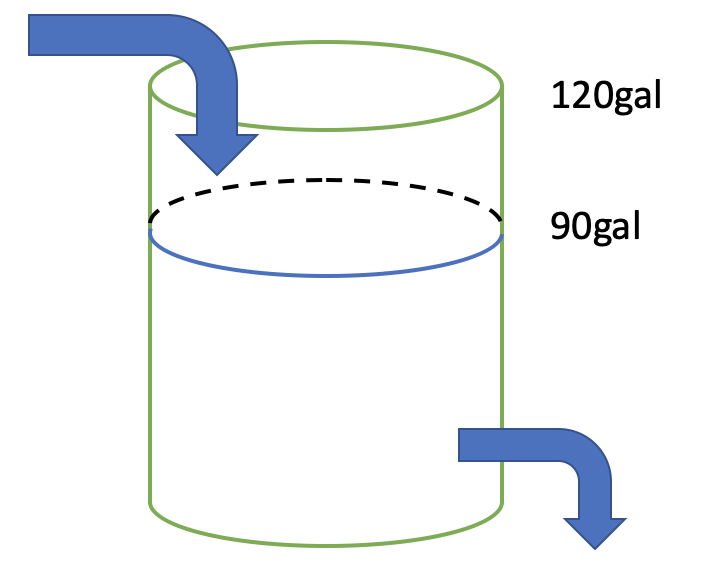
\includegraphics[width=5cm]{week2_wed_first}
\caption{First}
\end{figure}
Set $y(t)=$ the amount of salt at time $t$,\\ $V(t)=$the amount of brine at time $t$= 90 +$t$(gal)(t:minute)\\
\[\begin{aligned}y^\prime(t)&=2\text{kg/gal}\cdotp4\text{gal/min}-\frac{y(t)}{V(t)}\text{kg/gal}\cdotp3\text{gal/min}\\
&=8\text{kg/min}-3\frac{y(t)}{V(t)}\text{kg/min}
\end{aligned}
\]
\[y^\prime=8-3\frac{y}{90+t}
\]
\[y^\prime+\frac{3}{90+t}y=8
\]
By intergrating factor,
\[(e^{\int\frac{3}{90+t}\diff t}\cdotp y)^\prime=8e^{\int\frac{3}{90+t}\diff t}
\]
Try to simplify $e^{\int\frac{3}{90+t}\diff t}$;
\[\begin{aligned}\int\frac{3}{90+t}\diff t&=3ln|90+t|+\tilde{c}\\&=3ln(90+t)+\tilde{c}\end{aligned}
\]
Then,
\[e^{\int\frac{3}{90+t}\diff t}=(90+t)^3\cdotp c
\]
Integrate both sides,
\[(90+t)^3\cdotp c\cdotp y=8\int(90+t)^3\cdotp c\diff t
\]
\[(90+t)^3y=2\cdotp(90+t)^4+C
\]
\[y=2(90+t)+\frac{c}{(90+t)^3}
\]
\[y(0)=90=180+\frac{c}{90^3}\quad\Rightarrow\quad c=-90^4
\]
\[y=2(90+t)-\frac{90^4}{(90+t)^3}
\]
At $t=30$ the tank is full \& $y(30)=240-\frac{90^3}{120^3}\cdotp90$
\end{example}

\begin{example}[Persuit problem]
In a naval excercise, a distroyler $D$ is hunting a submarine $S$. Suppose $D$ at $(9,0)$ detects $S$ at $(0,0)$ \& at the same time $S$ detects $D$. Assuming that $S$ will dive immediately \& depart at full speed, $15$mile/hr in a straight course of unknown direction. What path should the destroyer $D$ follows to be certain of passing directly over the submarine $S$. If the speed of $D$ is $30$mile/hr at all time of the pursuit?
\begin{figure}[H]
\centering
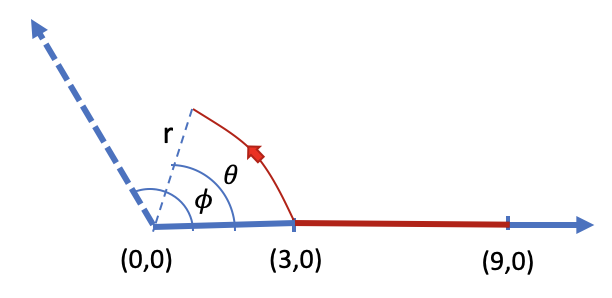
\includegraphics[width=8cm]{week2_wed_sec}
\caption{The path of destroyler in red.}
\end{figure}
Distance $D$ has travelled=$6+\int_0^\phi\sqrt{(r(\theta))^2+(r^\prime(\theta))^2}\diff\theta$.\\
Distance $S$ has travelled=$r(\phi)$.\\
For the speed of $D$ is twice than that of $S$, with the same period of time:
\[6+\int_0^\phi\sqrt{(r(\theta))^2+(r^\prime(\theta))^2}\diff\theta=2r(\phi)
\]
This isn't a form that can be dealt with. Differentiate both side,
\[\sqrt{(r(\phi))^2+(r^\prime(\phi))^2}=2r^\prime(\phi)
\]
\[(r(\phi))^2+(r^\prime(\phi))^2=4(r^\prime(\phi))^2
\]
\[r^\prime(\phi)=\pm\frac{1}{\sqrt{3}}r(\phi)
\]
W.L.O.G pick plus sign $\frac{r^\prime}{r}=\frac{1}{\sqrt{3}}$
\[lnr=\frac{1}{\sqrt{3}}\phi+\tilde{c}
\]
\[r=e^{\frac{\phi}{\sqrt{3}}}\cdotp c
\]
\[r(0)=3=c
\]
\[r(\phi)=3e^{\frac{\phi}{\sqrt{3}}}
\]
Given the direction $S$ take $\phi$, if $D$ want to be above it, they would reach each other at $(\phi,3e^{\frac{\phi}{\sqrt{3}}})$. This implies that if $D$ follows the path of 
$r(\theta)=3e^{\frac{\theta}{\sqrt{3}}}$, $D$ can catch $S$ whichever direction $S$ take.
\end{example}
\begin{remark}
There is a link about basic idea of how to compute the length of a curve:
\href{http://tutorial.math.lamar.edu/Classes/CalcII/ArcLength.aspx}{http://tutorial.math.lamar.edu/Classes/CalcII/ArcLength.aspx}. Check it if you are interested.
\end{remark}
\paragraph{Orthoganal trajectories} Given a family of curve $f(x,y,c)=0$. To find its orthoganal trajectories, the slope of the graph is needed. Differentiate $F$ by $x$;
\[F_x+F_yy_x=0
\]
Slope is $y_x=-\frac{F_x}{F_y}$. Then the slope of the graph that is orthoganal to the original one is \[y_x=\frac{F_y}{F_x}=\frac{\frac{\partial F}{\partial y}(x,y,c)}{\frac{\partial F}{\partial x}(x,y,c)}\]
\begin{example}
$y=cx^2$ $c$:parameter. To find another family of curves which is orthoganal to $y=cx^2$ whenever they intersect with each other.\\
$y=cx^2$, $\frac{\diff f}{\diff x}=2cx$ O.T. $\rightarrow \frac{\diff f}{\diff x}=\frac{-1}{2cx}=\frac{-1}{2\frac{y}{x^2}x}=-\frac{x}{2y}$ ( A separable equation)\\
$2y\diff y+x\diff x=0\quad\rightarrow\quad y^2+\frac{1}{2}x^2=c$
\end{example}



\chapter{Week8}

\section{Monday}\index{Monday_lecture}
\subsection{Euler's Equation}
Recall previous knowledge,
\[t^2y\pp+\alpha ty\p+\beta y=0\qquad t>0
\]
$y=t^r$ $\Rightarrow\qquad$ $r(r-1)+\alpha r+\beta=0$ \\
$r^2+(\alpha-1)r+\beta=0$\\
$r_1,r_2=\frac{-(\alpha-1)\pm\sqrt{(\alpha-1)-4\beta}}{2}$
\begin{enumerate}
\item $(\alpha-1)^2-4\beta>0$  two real roots, $y=c_1t^{r_1}+c_2t^{r_2}$
\item $(\alpha-1)^2-4\beta=0$ $r_1=r_2=r$, $y=c_1t^r+c_2t^rlnt$
\item $(\alpha-1)^2-4\beta<0$ $r=\lambda\pm i\mu$, $y=t^\lambda[c_1\cos(\mu lnt)+c_2\sin(\mu lnt)]$
\end{enumerate}

Some motivations of Euler's Equation: Bessel's equation of order $\frac{1}{2}$\\
\[t^2y\pp+ty\p+(t^2-\frac{1}{4})y=0
\]
There doesn't exist a solution with the form of $y=\sum_{n=0}^\infty a_nt^n$. When $t=0$ it's a first order differential equation, the solution of this equation is only at one point $t=0$ which doesn't make much sense. We call this a singular point. We need to do something to factor out singularity.\\
\paragraph{Generalization}
\[L[y]\equiv t^2y\pp+t[p_0+p_1t+p_2t^2+\dots]y\p+[q_0+q_1t+q_2t^2+\dots]y=0
\]
Method of Frobenius,
\[y=\sum_{n=0}^\infty a_nt^{n+r}
\]
\begin{remark}
$r$ can be $\mathbb{R}$.\\
In order to avoid ambiguity, $a_0\neq 0$. Otherwise, it becomes $y=\sum_{n=1}^\infty a_nt^{n+r}$ which are the same as $y=\sum_{n=0}^{\infty}b_nt^{n+r\p}$. As $r$ and $r\p=r+1$ need to be determined, we have $y=\sum_{n=1}^\infty a_nt^{n+r}$ with the first term equals to zero, and $y=\sum_{n=0}^{\infty}b_nt^{n+r\p}$ to represent the same thing. Simply put, $a_0\neq 0$
\end{remark}
\[y\p=\sum_{n=0}^\infty(n+r)a_nt^{n+r-1}
\]
\[y\pp=\sum_{n=0}^{\infty}(n+r)(n+r-1)a_nt^{n+r-2}
\]
\[\begin{aligned}L[y]&=\sum_0^\infty(n+r)(n+r-1)a_nt^{n+r}+(\sum_{m=0}^\infty p_mt^m)(\sum_0^\infty (n+r)a_nt^{n+r})+\sum_{m=0}^\infty q_nt^m\sum_0^\infty a_nt^{n+r}\\
&=r(r-1)a_0+p_0ra_0+q_0a_0+[(1+r)ra_1+p_0(1+r)a_1+p_1ra_0+q_0a_1q_1a_0]t+\dots\\
&=[r(r-1)+p_0r+q_0]a_0+\underline{[\{(1+r)r+p_0(1+r)+q_0\}a_1+\{p_1r+q_1\}a_0]t}+\dots\\
&\quad+\underline{[(k+r)(k+r-1)a_k+\sum_{m=0}^kp_m(k-m+r)a_{k-m}+\sum_{n=0}^kq_ma_{k-m}]t^k}+\dots
\end{aligned}
\]
In order to have a solution $L[y]=0$,
Indicial equation
\[F(r)=r(r-1)+p_0r+q_0=0
\]
\[F(r+1)a_1=-[p_1r+q_1]a_0
\]
retrieved from first underline.\\Let's rewrite second underline a little bit.
\[=[(k+r)(k+r-1)a_k+\sum_0^{k-l}p_{k-l}(l+r)a_l+p_0a_k(k+r)+\sum_{n=1}^kq_{k-l}a_l+q_0a_k]t^k
\]
\[F(r+k)a_k=-[\sum_0^{k-1}\{p_{k-l}(l+1)+q_{k-l}\}a_l]
\]
It is clear that all $a_n$ can be solved recursively.\\
If there exists two real roots $r_1\geq r_2$, then 
\begin{itemize}
\item $r_1>r_2$ and $r_1-r_2$ is  not a positive integer. We will have two solutions.
\item $r_1>r_2$ and $r_1-r_2$ is a positive ineger then, you need to check textbook for more information as this will not be tested in the final.
\item $r_1=r_2$ check \textsection 2.8.3 for more information.
\end{itemize}
\begin{example}
\[t^2y\pp+ty\p+(-\frac{1}{4}+t^2)y=0
\]
$p_0=1$, $p_1=p_2=\dots=0$; $q=-\frac{1}{4}$, $q_1=0$, $q_2=1$, $q_3=0$\\Look at $L[y]\equiv t^2y\pp+t[p_0+p_1t+p_2t^2+\dots]y\p+[q_0+q_1t+q_2t^2+\dots]y=0$. You will know how we get all those stuffs.\\
$r(r-1)+r-\frac{1}{4}=0$, $r=\pm\frac{1}{2}$\\
First look at the first case $r=r_1=\frac{1}{2}$\\
$F(q+\frac{1}{2})a_1=0\Rightarrow a_1=0\dots(1)$ (We just pluge those stuffs in $F(r+1)a_1=-[p_1r+q_1]a_0$. \\
$F(k+r)a_k=k(k+1)a_k=-a_{k-2}\quad\Rightarrow ak=-\frac{1}{(k+1)ka_{k-2}}\dots(2)$  (As $F(k+r)=(r+k)^2-\frac{1}{4}=k(k+1)$)\\
With (1) and (2), we get $a_3=a_5=\dots=0$
\[a_2=-\frac{1}{3!}a_0
\]
\[a_4=-\frac{1}{5\cdot4}a_2=\frac{1}{5!}a_0
\]
\[a_{2n}=\frac{(-1)^n}{(2n+1)!}a_0
\]
\[y_1=a_0t^{\frac{1}{2}}(1-\frac{1}{3!}t^2+\frac{1}{5!}t^2-\dots)
\]
\[y_1=a_0t^{-\frac{1}{2}}\sin t
\]
$r_2=-\frac{1}{2}$
\[F(1+r_2)a_1=F(\frac{1}{2})a_1=0
\]
It's lucky both sides are equal to zero, else we cannot solve the second solution in this way.
\[F(k+r_2)=k(k-1)a_k=-q_2a_{k-2}=-a_{k-2}
\]
\[a_k=-\frac{1}{(k-1)k}a_{k-2}
\]
\[a_2=-\frac{1}{2}a_0
\]
\[a_4=-\frac{a_4}{4\cdot3}a_2=\frac{1}{4!}a_0
\]
\[a_6=-\frac{a_4}{6\cdot5}=-\frac{1}{6!}a_0
\]
\[y_2=t^{-\frac{1}{2}}a_0[1-\frac{1}{2!}t^2+\frac{1}{4!}t^4+\dots]=a_0t^{-\frac{1}{2}}\cos t
\]
Therefore, the general solutions is $y=\frac{1}{\sqrt{t}}(c_1\cos t+c_2\sin t)$
\end{example}



\section{Wednesday}\index{Wednesday_lecture}
\subsection{Application}
\paragraph{Mixture problem}There are two things that you need to bear in mind: \\\textcolor{red}{$\frac{\diff y}{\diff t}=$ input rate - output rate}, carry the units.

\begin{example}
A 120-gal tank initially contain 90kg salt dissoved in 90-gal of water. Brine containing 2kg/gal of salt flows into the tank at the water. Brine containing 2kg/gal of salt flows into the tank at the rate of 4gal/min, \& the well-stirned mixture flows out at the rate of 3 gal/min. How much salt does the tank contain when it is full?
\begin{figure}[H]
\centering
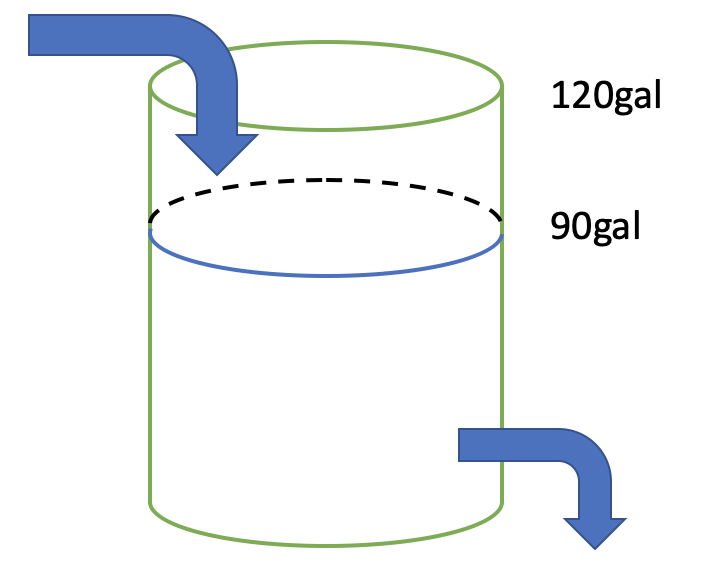
\includegraphics[width=5cm]{week2_wed_first}
\caption{First}
\end{figure}
Set $y(t)=$ the amount of salt at time $t$,\\ $V(t)=$the amount of brine at time $t$= 90 +$t$(gal)(t:minute)\\
\[\begin{aligned}y^\prime(t)&=2\text{kg/gal}\cdotp4\text{gal/min}-\frac{y(t)}{V(t)}\text{kg/gal}\cdotp3\text{gal/min}\\
&=8\text{kg/min}-3\frac{y(t)}{V(t)}\text{kg/min}
\end{aligned}
\]
\[y^\prime=8-3\frac{y}{90+t}
\]
\[y^\prime+\frac{3}{90+t}y=8
\]
By intergrating factor,
\[(e^{\int\frac{3}{90+t}\diff t}\cdotp y)^\prime=8e^{\int\frac{3}{90+t}\diff t}
\]
Try to simplify $e^{\int\frac{3}{90+t}\diff t}$;
\[\begin{aligned}\int\frac{3}{90+t}\diff t&=3ln|90+t|+\tilde{c}\\&=3ln(90+t)+\tilde{c}\end{aligned}
\]
Then,
\[e^{\int\frac{3}{90+t}\diff t}=(90+t)^3\cdotp c
\]
Integrate both sides,
\[(90+t)^3\cdotp c\cdotp y=8\int(90+t)^3\cdotp c\diff t
\]
\[(90+t)^3y=2\cdotp(90+t)^4+C
\]
\[y=2(90+t)+\frac{c}{(90+t)^3}
\]
\[y(0)=90=180+\frac{c}{90^3}\quad\Rightarrow\quad c=-90^4
\]
\[y=2(90+t)-\frac{90^4}{(90+t)^3}
\]
At $t=30$ the tank is full \& $y(30)=240-\frac{90^3}{120^3}\cdotp90$
\end{example}

\begin{example}[Persuit problem]
In a naval excercise, a distroyler $D$ is hunting a submarine $S$. Suppose $D$ at $(9,0)$ detects $S$ at $(0,0)$ \& at the same time $S$ detects $D$. Assuming that $S$ will dive immediately \& depart at full speed, $15$mile/hr in a straight course of unknown direction. What path should the destroyer $D$ follows to be certain of passing directly over the submarine $S$. If the speed of $D$ is $30$mile/hr at all time of the pursuit?
\begin{figure}[H]
\centering
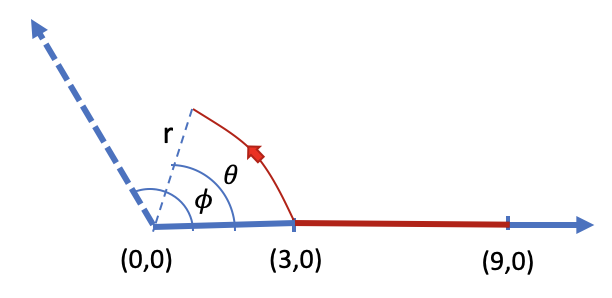
\includegraphics[width=8cm]{week2_wed_sec}
\caption{The path of destroyler in red.}
\end{figure}
Distance $D$ has travelled=$6+\int_0^\phi\sqrt{(r(\theta))^2+(r^\prime(\theta))^2}\diff\theta$.\\
Distance $S$ has travelled=$r(\phi)$.\\
For the speed of $D$ is twice than that of $S$, with the same period of time:
\[6+\int_0^\phi\sqrt{(r(\theta))^2+(r^\prime(\theta))^2}\diff\theta=2r(\phi)
\]
This isn't a form that can be dealt with. Differentiate both side,
\[\sqrt{(r(\phi))^2+(r^\prime(\phi))^2}=2r^\prime(\phi)
\]
\[(r(\phi))^2+(r^\prime(\phi))^2=4(r^\prime(\phi))^2
\]
\[r^\prime(\phi)=\pm\frac{1}{\sqrt{3}}r(\phi)
\]
W.L.O.G pick plus sign $\frac{r^\prime}{r}=\frac{1}{\sqrt{3}}$
\[lnr=\frac{1}{\sqrt{3}}\phi+\tilde{c}
\]
\[r=e^{\frac{\phi}{\sqrt{3}}}\cdotp c
\]
\[r(0)=3=c
\]
\[r(\phi)=3e^{\frac{\phi}{\sqrt{3}}}
\]
Given the direction $S$ take $\phi$, if $D$ want to be above it, they would reach each other at $(\phi,3e^{\frac{\phi}{\sqrt{3}}})$. This implies that if $D$ follows the path of 
$r(\theta)=3e^{\frac{\theta}{\sqrt{3}}}$, $D$ can catch $S$ whichever direction $S$ take.
\end{example}
\begin{remark}
There is a link about basic idea of how to compute the length of a curve:
\href{http://tutorial.math.lamar.edu/Classes/CalcII/ArcLength.aspx}{http://tutorial.math.lamar.edu/Classes/CalcII/ArcLength.aspx}. Check it if you are interested.
\end{remark}
\paragraph{Orthoganal trajectories} Given a family of curve $f(x,y,c)=0$. To find its orthoganal trajectories, the slope of the graph is needed. Differentiate $F$ by $x$;
\[F_x+F_yy_x=0
\]
Slope is $y_x=-\frac{F_x}{F_y}$. Then the slope of the graph that is orthoganal to the original one is \[y_x=\frac{F_y}{F_x}=\frac{\frac{\partial F}{\partial y}(x,y,c)}{\frac{\partial F}{\partial x}(x,y,c)}\]
\begin{example}
$y=cx^2$ $c$:parameter. To find another family of curves which is orthoganal to $y=cx^2$ whenever they intersect with each other.\\
$y=cx^2$, $\frac{\diff f}{\diff x}=2cx$ O.T. $\rightarrow \frac{\diff f}{\diff x}=\frac{-1}{2cx}=\frac{-1}{2\frac{y}{x^2}x}=-\frac{x}{2y}$ ( A separable equation)\\
$2y\diff y+x\diff x=0\quad\rightarrow\quad y^2+\frac{1}{2}x^2=c$
\end{example}



\chapter{Week8}

\section{Monday}\index{Monday_lecture}
\subsection{Euler's Equation}
Recall previous knowledge,
\[t^2y\pp+\alpha ty\p+\beta y=0\qquad t>0
\]
$y=t^r$ $\Rightarrow\qquad$ $r(r-1)+\alpha r+\beta=0$ \\
$r^2+(\alpha-1)r+\beta=0$\\
$r_1,r_2=\frac{-(\alpha-1)\pm\sqrt{(\alpha-1)-4\beta}}{2}$
\begin{enumerate}
\item $(\alpha-1)^2-4\beta>0$  two real roots, $y=c_1t^{r_1}+c_2t^{r_2}$
\item $(\alpha-1)^2-4\beta=0$ $r_1=r_2=r$, $y=c_1t^r+c_2t^rlnt$
\item $(\alpha-1)^2-4\beta<0$ $r=\lambda\pm i\mu$, $y=t^\lambda[c_1\cos(\mu lnt)+c_2\sin(\mu lnt)]$
\end{enumerate}

Some motivations of Euler's Equation: Bessel's equation of order $\frac{1}{2}$\\
\[t^2y\pp+ty\p+(t^2-\frac{1}{4})y=0
\]
There doesn't exist a solution with the form of $y=\sum_{n=0}^\infty a_nt^n$. When $t=0$ it's a first order differential equation, the solution of this equation is only at one point $t=0$ which doesn't make much sense. We call this a singular point. We need to do something to factor out singularity.\\
\paragraph{Generalization}
\[L[y]\equiv t^2y\pp+t[p_0+p_1t+p_2t^2+\dots]y\p+[q_0+q_1t+q_2t^2+\dots]y=0
\]
Method of Frobenius,
\[y=\sum_{n=0}^\infty a_nt^{n+r}
\]
\begin{remark}
$r$ can be $\mathbb{R}$.\\
In order to avoid ambiguity, $a_0\neq 0$. Otherwise, it becomes $y=\sum_{n=1}^\infty a_nt^{n+r}$ which are the same as $y=\sum_{n=0}^{\infty}b_nt^{n+r\p}$. As $r$ and $r\p=r+1$ need to be determined, we have $y=\sum_{n=1}^\infty a_nt^{n+r}$ with the first term equals to zero, and $y=\sum_{n=0}^{\infty}b_nt^{n+r\p}$ to represent the same thing. Simply put, $a_0\neq 0$
\end{remark}
\[y\p=\sum_{n=0}^\infty(n+r)a_nt^{n+r-1}
\]
\[y\pp=\sum_{n=0}^{\infty}(n+r)(n+r-1)a_nt^{n+r-2}
\]
\[\begin{aligned}L[y]&=\sum_0^\infty(n+r)(n+r-1)a_nt^{n+r}+(\sum_{m=0}^\infty p_mt^m)(\sum_0^\infty (n+r)a_nt^{n+r})+\sum_{m=0}^\infty q_nt^m\sum_0^\infty a_nt^{n+r}\\
&=r(r-1)a_0+p_0ra_0+q_0a_0+[(1+r)ra_1+p_0(1+r)a_1+p_1ra_0+q_0a_1q_1a_0]t+\dots\\
&=[r(r-1)+p_0r+q_0]a_0+\underline{[\{(1+r)r+p_0(1+r)+q_0\}a_1+\{p_1r+q_1\}a_0]t}+\dots\\
&\quad+\underline{[(k+r)(k+r-1)a_k+\sum_{m=0}^kp_m(k-m+r)a_{k-m}+\sum_{n=0}^kq_ma_{k-m}]t^k}+\dots
\end{aligned}
\]
In order to have a solution $L[y]=0$,
Indicial equation
\[F(r)=r(r-1)+p_0r+q_0=0
\]
\[F(r+1)a_1=-[p_1r+q_1]a_0
\]
retrieved from first underline.\\Let's rewrite second underline a little bit.
\[=[(k+r)(k+r-1)a_k+\sum_0^{k-l}p_{k-l}(l+r)a_l+p_0a_k(k+r)+\sum_{n=1}^kq_{k-l}a_l+q_0a_k]t^k
\]
\[F(r+k)a_k=-[\sum_0^{k-1}\{p_{k-l}(l+1)+q_{k-l}\}a_l]
\]
It is clear that all $a_n$ can be solved recursively.\\
If there exists two real roots $r_1\geq r_2$, then 
\begin{itemize}
\item $r_1>r_2$ and $r_1-r_2$ is  not a positive integer. We will have two solutions.
\item $r_1>r_2$ and $r_1-r_2$ is a positive ineger then, you need to check textbook for more information as this will not be tested in the final.
\item $r_1=r_2$ check \textsection 2.8.3 for more information.
\end{itemize}
\begin{example}
\[t^2y\pp+ty\p+(-\frac{1}{4}+t^2)y=0
\]
$p_0=1$, $p_1=p_2=\dots=0$; $q=-\frac{1}{4}$, $q_1=0$, $q_2=1$, $q_3=0$\\Look at $L[y]\equiv t^2y\pp+t[p_0+p_1t+p_2t^2+\dots]y\p+[q_0+q_1t+q_2t^2+\dots]y=0$. You will know how we get all those stuffs.\\
$r(r-1)+r-\frac{1}{4}=0$, $r=\pm\frac{1}{2}$\\
First look at the first case $r=r_1=\frac{1}{2}$\\
$F(q+\frac{1}{2})a_1=0\Rightarrow a_1=0\dots(1)$ (We just pluge those stuffs in $F(r+1)a_1=-[p_1r+q_1]a_0$. \\
$F(k+r)a_k=k(k+1)a_k=-a_{k-2}\quad\Rightarrow ak=-\frac{1}{(k+1)ka_{k-2}}\dots(2)$  (As $F(k+r)=(r+k)^2-\frac{1}{4}=k(k+1)$)\\
With (1) and (2), we get $a_3=a_5=\dots=0$
\[a_2=-\frac{1}{3!}a_0
\]
\[a_4=-\frac{1}{5\cdot4}a_2=\frac{1}{5!}a_0
\]
\[a_{2n}=\frac{(-1)^n}{(2n+1)!}a_0
\]
\[y_1=a_0t^{\frac{1}{2}}(1-\frac{1}{3!}t^2+\frac{1}{5!}t^2-\dots)
\]
\[y_1=a_0t^{-\frac{1}{2}}\sin t
\]
$r_2=-\frac{1}{2}$
\[F(1+r_2)a_1=F(\frac{1}{2})a_1=0
\]
It's lucky both sides are equal to zero, else we cannot solve the second solution in this way.
\[F(k+r_2)=k(k-1)a_k=-q_2a_{k-2}=-a_{k-2}
\]
\[a_k=-\frac{1}{(k-1)k}a_{k-2}
\]
\[a_2=-\frac{1}{2}a_0
\]
\[a_4=-\frac{a_4}{4\cdot3}a_2=\frac{1}{4!}a_0
\]
\[a_6=-\frac{a_4}{6\cdot5}=-\frac{1}{6!}a_0
\]
\[y_2=t^{-\frac{1}{2}}a_0[1-\frac{1}{2!}t^2+\frac{1}{4!}t^4+\dots]=a_0t^{-\frac{1}{2}}\cos t
\]
Therefore, the general solutions is $y=\frac{1}{\sqrt{t}}(c_1\cos t+c_2\sin t)$
\end{example}



\section{Wednesday}\index{Wednesday_lecture}
\subsection{Application}
\paragraph{Mixture problem}There are two things that you need to bear in mind: \\\textcolor{red}{$\frac{\diff y}{\diff t}=$ input rate - output rate}, carry the units.

\begin{example}
A 120-gal tank initially contain 90kg salt dissoved in 90-gal of water. Brine containing 2kg/gal of salt flows into the tank at the water. Brine containing 2kg/gal of salt flows into the tank at the rate of 4gal/min, \& the well-stirned mixture flows out at the rate of 3 gal/min. How much salt does the tank contain when it is full?
\begin{figure}[H]
\centering
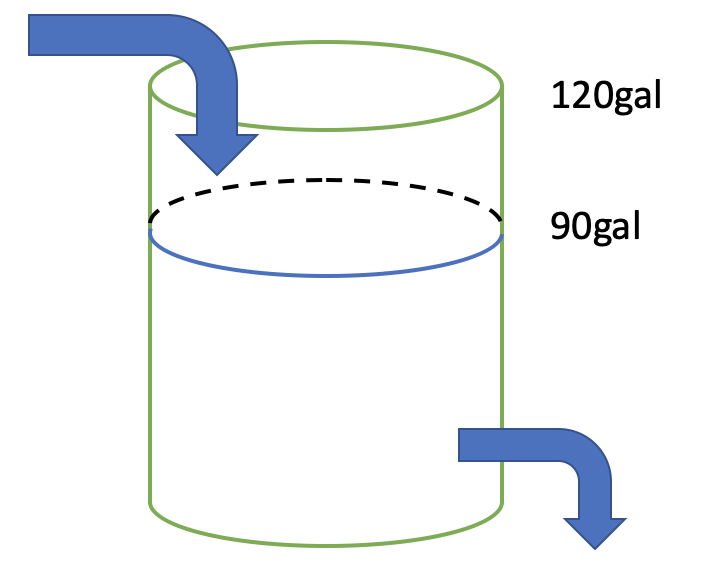
\includegraphics[width=5cm]{week2_wed_first}
\caption{First}
\end{figure}
Set $y(t)=$ the amount of salt at time $t$,\\ $V(t)=$the amount of brine at time $t$= 90 +$t$(gal)(t:minute)\\
\[\begin{aligned}y^\prime(t)&=2\text{kg/gal}\cdotp4\text{gal/min}-\frac{y(t)}{V(t)}\text{kg/gal}\cdotp3\text{gal/min}\\
&=8\text{kg/min}-3\frac{y(t)}{V(t)}\text{kg/min}
\end{aligned}
\]
\[y^\prime=8-3\frac{y}{90+t}
\]
\[y^\prime+\frac{3}{90+t}y=8
\]
By intergrating factor,
\[(e^{\int\frac{3}{90+t}\diff t}\cdotp y)^\prime=8e^{\int\frac{3}{90+t}\diff t}
\]
Try to simplify $e^{\int\frac{3}{90+t}\diff t}$;
\[\begin{aligned}\int\frac{3}{90+t}\diff t&=3ln|90+t|+\tilde{c}\\&=3ln(90+t)+\tilde{c}\end{aligned}
\]
Then,
\[e^{\int\frac{3}{90+t}\diff t}=(90+t)^3\cdotp c
\]
Integrate both sides,
\[(90+t)^3\cdotp c\cdotp y=8\int(90+t)^3\cdotp c\diff t
\]
\[(90+t)^3y=2\cdotp(90+t)^4+C
\]
\[y=2(90+t)+\frac{c}{(90+t)^3}
\]
\[y(0)=90=180+\frac{c}{90^3}\quad\Rightarrow\quad c=-90^4
\]
\[y=2(90+t)-\frac{90^4}{(90+t)^3}
\]
At $t=30$ the tank is full \& $y(30)=240-\frac{90^3}{120^3}\cdotp90$
\end{example}

\begin{example}[Persuit problem]
In a naval excercise, a distroyler $D$ is hunting a submarine $S$. Suppose $D$ at $(9,0)$ detects $S$ at $(0,0)$ \& at the same time $S$ detects $D$. Assuming that $S$ will dive immediately \& depart at full speed, $15$mile/hr in a straight course of unknown direction. What path should the destroyer $D$ follows to be certain of passing directly over the submarine $S$. If the speed of $D$ is $30$mile/hr at all time of the pursuit?
\begin{figure}[H]
\centering
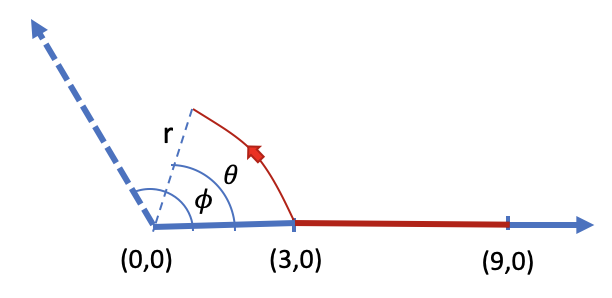
\includegraphics[width=8cm]{week2_wed_sec}
\caption{The path of destroyler in red.}
\end{figure}
Distance $D$ has travelled=$6+\int_0^\phi\sqrt{(r(\theta))^2+(r^\prime(\theta))^2}\diff\theta$.\\
Distance $S$ has travelled=$r(\phi)$.\\
For the speed of $D$ is twice than that of $S$, with the same period of time:
\[6+\int_0^\phi\sqrt{(r(\theta))^2+(r^\prime(\theta))^2}\diff\theta=2r(\phi)
\]
This isn't a form that can be dealt with. Differentiate both side,
\[\sqrt{(r(\phi))^2+(r^\prime(\phi))^2}=2r^\prime(\phi)
\]
\[(r(\phi))^2+(r^\prime(\phi))^2=4(r^\prime(\phi))^2
\]
\[r^\prime(\phi)=\pm\frac{1}{\sqrt{3}}r(\phi)
\]
W.L.O.G pick plus sign $\frac{r^\prime}{r}=\frac{1}{\sqrt{3}}$
\[lnr=\frac{1}{\sqrt{3}}\phi+\tilde{c}
\]
\[r=e^{\frac{\phi}{\sqrt{3}}}\cdotp c
\]
\[r(0)=3=c
\]
\[r(\phi)=3e^{\frac{\phi}{\sqrt{3}}}
\]
Given the direction $S$ take $\phi$, if $D$ want to be above it, they would reach each other at $(\phi,3e^{\frac{\phi}{\sqrt{3}}})$. This implies that if $D$ follows the path of 
$r(\theta)=3e^{\frac{\theta}{\sqrt{3}}}$, $D$ can catch $S$ whichever direction $S$ take.
\end{example}
\begin{remark}
There is a link about basic idea of how to compute the length of a curve:
\href{http://tutorial.math.lamar.edu/Classes/CalcII/ArcLength.aspx}{http://tutorial.math.lamar.edu/Classes/CalcII/ArcLength.aspx}. Check it if you are interested.
\end{remark}
\paragraph{Orthoganal trajectories} Given a family of curve $f(x,y,c)=0$. To find its orthoganal trajectories, the slope of the graph is needed. Differentiate $F$ by $x$;
\[F_x+F_yy_x=0
\]
Slope is $y_x=-\frac{F_x}{F_y}$. Then the slope of the graph that is orthoganal to the original one is \[y_x=\frac{F_y}{F_x}=\frac{\frac{\partial F}{\partial y}(x,y,c)}{\frac{\partial F}{\partial x}(x,y,c)}\]
\begin{example}
$y=cx^2$ $c$:parameter. To find another family of curves which is orthoganal to $y=cx^2$ whenever they intersect with each other.\\
$y=cx^2$, $\frac{\diff f}{\diff x}=2cx$ O.T. $\rightarrow \frac{\diff f}{\diff x}=\frac{-1}{2cx}=\frac{-1}{2\frac{y}{x^2}x}=-\frac{x}{2y}$ ( A separable equation)\\
$2y\diff y+x\diff x=0\quad\rightarrow\quad y^2+\frac{1}{2}x^2=c$
\end{example}




\chapter{Week4}

\section{Monday}\index{Monday_lecture}
\subsection{Which part of motion last longer?}
Now we consider throwing a ball straight upward. At first, it will go up. Then because of gravity, it will goes down. If air friction is considered, which part of motion experience more time?
\begin{figure}[H]
\centering
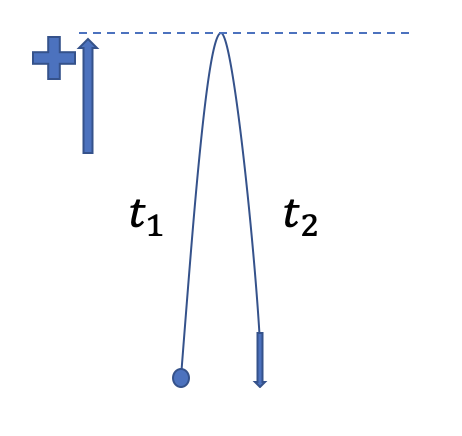
\includegraphics[width=4cm]{week4}
\end{figure}
In order to make content complete, first, let's consider the procedure without any friction.
\[mv^\prime=-mg
\]
\[v(t)=-gt+v_0\]
,where $v_0$ is a initial velocity.
\[v(T_{\textit{up}})=v_0-gT_{\textit{up}}
\]
\[T_{\textit{up}}=\frac{v_0}{g},~T_{\textit{down}}=\frac{v_0}{g}
\]
Now let's consider the case where air friction exists. By recent discovery, relationship between air friction and the speed of the objection is; $F=kv^{p}$ where $p$ ($
1\leq p\leq2$) is a constant related to the speed, i.e. when the speed is high, $p$ is aproximately 2; otherwise, $p$ is more close to 1 and $k$ is a constant related to the shape of the object.
\[F=-kv|v|
\](This hold nomatter $p$ is equal to 1 or 2 where $v$ is a vector.)
To make our life easier, take $p=1$,
\[mv^\prime=-mg-kv
\]
\[v^\prime=-g-\frac{k}{m}v
\]
Let $\rho=\frac{k}{m}$
\[v^\prime+\rho v=-g
\]
\[e^{\rho t}(v^\prime+\rho v)=-ge^{\rho t}\]
Take integral on both side of the equation,
\[e^{\rho t}v(t)-v(0)=-\int_0^tge^{\rho s}\diff s=-\frac{g}{\rho}(e^{\rho t}-1)
\]
\[e^{\rho t}v(t)=v_0+\frac{g}{\rho}-\frac{g}{\rho}e^{\rho t}
\]
\[v(t)=e^{-\rho t}(v_0+\frac{g}{\rho})-\frac{g}{\rho}
\]
\[v(T_{\textit{up}})=0=e^{-\rho T_{\textit{up}}}(v_0+\frac{g}{\rho})-\frac{g}{\rho}
\]
\[v_0+\frac{g}{\rho}=\frac{g}{\rho}e^{\rho T_{\textit{up}}}
\]
\[\boxed{e^{\rho T_{\textit{up}}}=\frac{v_0+\frac{g}{\rho}}{\frac{g}{\rho}}}
\]
Max height $H=\int_0^{T_{\textit{up}}}v(t)\diff t$
\[T_{\textit{down}}=T_{\textit{total}}-T_{\textit{up}}
\]
$T_{\textit{total}}$ is given by $h(T_{\textit{total}})=0$, where $h(t)=\int_0^tv(s)\diff s$
\[h(t)=\int_0^t[e^{\rho t}(v_0+\frac{g}{\rho})-\frac{g}{\rho}]\diff s=-\frac{1}{\rho}(e^{-\rho t}-1)(v_0+\frac{g}{\rho})-\frac{g}{\rho}t
\]
$h(total)=h(0)$ is given by $\frac{1}{\rho}(e^{-\rho T_{\textit{total}}}-1)(v_0+\frac{g}{\rho})=\frac{g}{\rho}T_{\textit{total}}$\\
Question: Can you see $T_{\textit{up}}<T_{\textit{down}}$?\\
Answer: Interesting.\\
$k=0$(no air)\\
$T_{\textit{up}}=\frac{v_0}{g}$
\[\begin{aligned}
H&=\int_0^{T_{\textit{up}}}(-gt+v_0)\diff t\\
&=(-\frac{g}{2}t^2+v_0t)|_0^{\frac{v_0}{g}}\\
&=\frac{v_0^2}{g}-\frac{g}{2}(\frac{v_0}{g})^2
=\frac{v_0^2}{2g}
\end{aligned}
\]
\[T_{\textit{total}}=2\frac{v_0}{g}
\]
$k>0$ $\quad T_{\textit{up}}=\frac{1}{\rho}ln(1+\frac{g}{\rho}v_0) \quad H=h_0+\frac{v_0}{\rho}-\frac{g}{\rho}T_{\textit{up}}$ \\
Question: please examine when $\rho\rightarrow 0$ everything goes to the right quantity.
\begin{example}
A bolt shot straight upward with initial velocity 49m/sec from a cross bow at ground level. With air resistance take into account. Assuming the constant $\rho=0.04$ (and $\rho=0.2$ for comparison). Compute $T_{\textit{up}}$ and $T_{\textit{down}}$.\\
$P=0.04$ $v_0=49$, $g=9.8m/sec^2$\\
\[T_{\textit{up}}=\frac{1}{0.04}ln(1+0.04\cdot5)=\frac{1}{0.04}ln(1.2)\approx4.56sec
\]
\[T_{\textit{total}}\approx9.41sec
\]
\[T_{\textit{down}}=9.41-4.56=4.85sec
\]
$p=0.2$
\[T_{\textit{up}}=3.47
\]
\[T_{\textit{total}}=8sec
\]
\[T_{\textit{down}}=4.53sec
\]
Indeed, upper time is shorter than downward time.

\end{example}




\section{Wednesday}\index{Wednesday_lecture}
\subsection{Application}
\paragraph{Mixture problem}There are two things that you need to bear in mind: \\\textcolor{red}{$\frac{\diff y}{\diff t}=$ input rate - output rate}, carry the units.

\begin{example}
A 120-gal tank initially contain 90kg salt dissoved in 90-gal of water. Brine containing 2kg/gal of salt flows into the tank at the water. Brine containing 2kg/gal of salt flows into the tank at the rate of 4gal/min, \& the well-stirned mixture flows out at the rate of 3 gal/min. How much salt does the tank contain when it is full?
\begin{figure}[H]
\centering
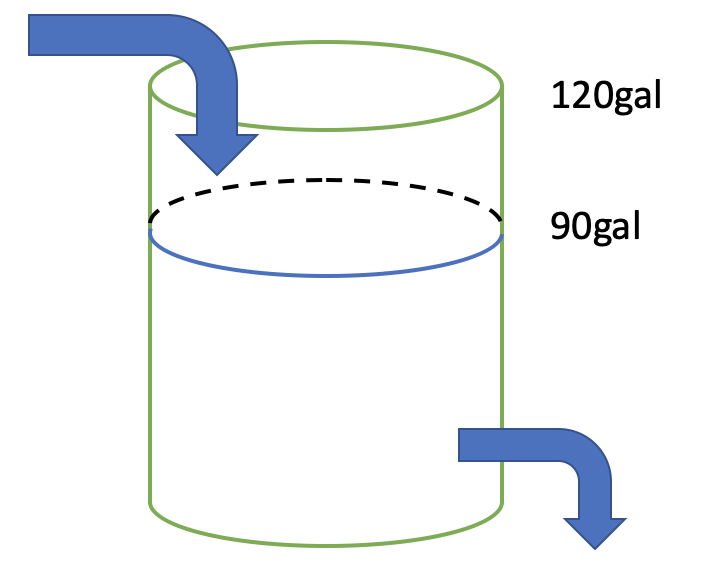
\includegraphics[width=5cm]{week2_wed_first}
\caption{First}
\end{figure}
Set $y(t)=$ the amount of salt at time $t$,\\ $V(t)=$the amount of brine at time $t$= 90 +$t$(gal)(t:minute)\\
\[\begin{aligned}y^\prime(t)&=2\text{kg/gal}\cdotp4\text{gal/min}-\frac{y(t)}{V(t)}\text{kg/gal}\cdotp3\text{gal/min}\\
&=8\text{kg/min}-3\frac{y(t)}{V(t)}\text{kg/min}
\end{aligned}
\]
\[y^\prime=8-3\frac{y}{90+t}
\]
\[y^\prime+\frac{3}{90+t}y=8
\]
By intergrating factor,
\[(e^{\int\frac{3}{90+t}\diff t}\cdotp y)^\prime=8e^{\int\frac{3}{90+t}\diff t}
\]
Try to simplify $e^{\int\frac{3}{90+t}\diff t}$;
\[\begin{aligned}\int\frac{3}{90+t}\diff t&=3ln|90+t|+\tilde{c}\\&=3ln(90+t)+\tilde{c}\end{aligned}
\]
Then,
\[e^{\int\frac{3}{90+t}\diff t}=(90+t)^3\cdotp c
\]
Integrate both sides,
\[(90+t)^3\cdotp c\cdotp y=8\int(90+t)^3\cdotp c\diff t
\]
\[(90+t)^3y=2\cdotp(90+t)^4+C
\]
\[y=2(90+t)+\frac{c}{(90+t)^3}
\]
\[y(0)=90=180+\frac{c}{90^3}\quad\Rightarrow\quad c=-90^4
\]
\[y=2(90+t)-\frac{90^4}{(90+t)^3}
\]
At $t=30$ the tank is full \& $y(30)=240-\frac{90^3}{120^3}\cdotp90$
\end{example}

\begin{example}[Persuit problem]
In a naval excercise, a distroyler $D$ is hunting a submarine $S$. Suppose $D$ at $(9,0)$ detects $S$ at $(0,0)$ \& at the same time $S$ detects $D$. Assuming that $S$ will dive immediately \& depart at full speed, $15$mile/hr in a straight course of unknown direction. What path should the destroyer $D$ follows to be certain of passing directly over the submarine $S$. If the speed of $D$ is $30$mile/hr at all time of the pursuit?
\begin{figure}[H]
\centering
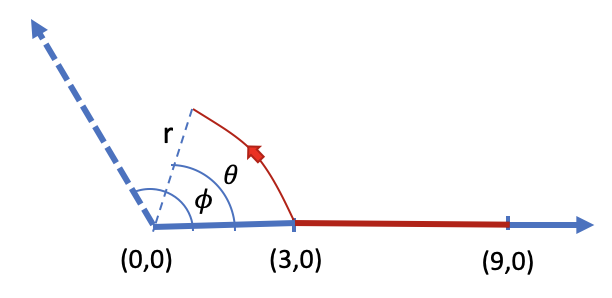
\includegraphics[width=8cm]{week2_wed_sec}
\caption{The path of destroyler in red.}
\end{figure}
Distance $D$ has travelled=$6+\int_0^\phi\sqrt{(r(\theta))^2+(r^\prime(\theta))^2}\diff\theta$.\\
Distance $S$ has travelled=$r(\phi)$.\\
For the speed of $D$ is twice than that of $S$, with the same period of time:
\[6+\int_0^\phi\sqrt{(r(\theta))^2+(r^\prime(\theta))^2}\diff\theta=2r(\phi)
\]
This isn't a form that can be dealt with. Differentiate both side,
\[\sqrt{(r(\phi))^2+(r^\prime(\phi))^2}=2r^\prime(\phi)
\]
\[(r(\phi))^2+(r^\prime(\phi))^2=4(r^\prime(\phi))^2
\]
\[r^\prime(\phi)=\pm\frac{1}{\sqrt{3}}r(\phi)
\]
W.L.O.G pick plus sign $\frac{r^\prime}{r}=\frac{1}{\sqrt{3}}$
\[lnr=\frac{1}{\sqrt{3}}\phi+\tilde{c}
\]
\[r=e^{\frac{\phi}{\sqrt{3}}}\cdotp c
\]
\[r(0)=3=c
\]
\[r(\phi)=3e^{\frac{\phi}{\sqrt{3}}}
\]
Given the direction $S$ take $\phi$, if $D$ want to be above it, they would reach each other at $(\phi,3e^{\frac{\phi}{\sqrt{3}}})$. This implies that if $D$ follows the path of 
$r(\theta)=3e^{\frac{\theta}{\sqrt{3}}}$, $D$ can catch $S$ whichever direction $S$ take.
\end{example}
\begin{remark}
There is a link about basic idea of how to compute the length of a curve:
\href{http://tutorial.math.lamar.edu/Classes/CalcII/ArcLength.aspx}{http://tutorial.math.lamar.edu/Classes/CalcII/ArcLength.aspx}. Check it if you are interested.
\end{remark}
\paragraph{Orthoganal trajectories} Given a family of curve $f(x,y,c)=0$. To find its orthoganal trajectories, the slope of the graph is needed. Differentiate $F$ by $x$;
\[F_x+F_yy_x=0
\]
Slope is $y_x=-\frac{F_x}{F_y}$. Then the slope of the graph that is orthoganal to the original one is \[y_x=\frac{F_y}{F_x}=\frac{\frac{\partial F}{\partial y}(x,y,c)}{\frac{\partial F}{\partial x}(x,y,c)}\]
\begin{example}
$y=cx^2$ $c$:parameter. To find another family of curves which is orthoganal to $y=cx^2$ whenever they intersect with each other.\\
$y=cx^2$, $\frac{\diff f}{\diff x}=2cx$ O.T. $\rightarrow \frac{\diff f}{\diff x}=\frac{-1}{2cx}=\frac{-1}{2\frac{y}{x^2}x}=-\frac{x}{2y}$ ( A separable equation)\\
$2y\diff y+x\diff x=0\quad\rightarrow\quad y^2+\frac{1}{2}x^2=c$
\end{example}




\section{Wednesday}\index{Wednesday_lecture}
\subsection{Laplace Transformation}
\[\lapl{f}(s)=\int_0^\infty e^{-st}f(t)\diff t
\]
\[|f(t)\leq Me^{ct}|\qquad\text{for t large, } s>c
\]
Heariside function $H(t)$
\begin{figure}[H]
\centering
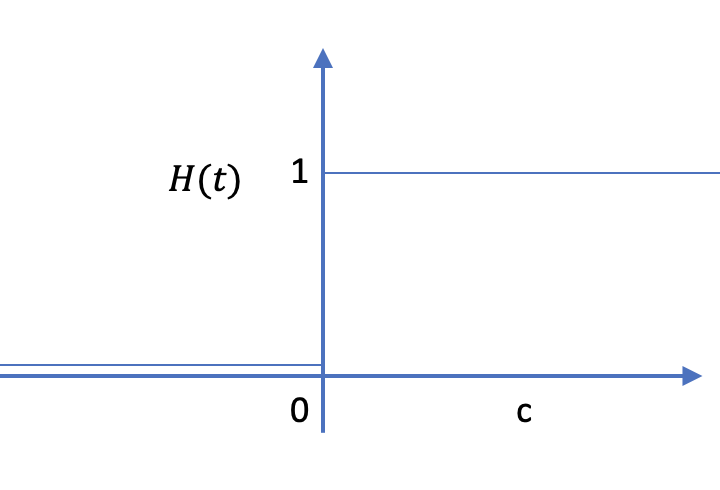
\includegraphics[width=6cm]{week9_1}
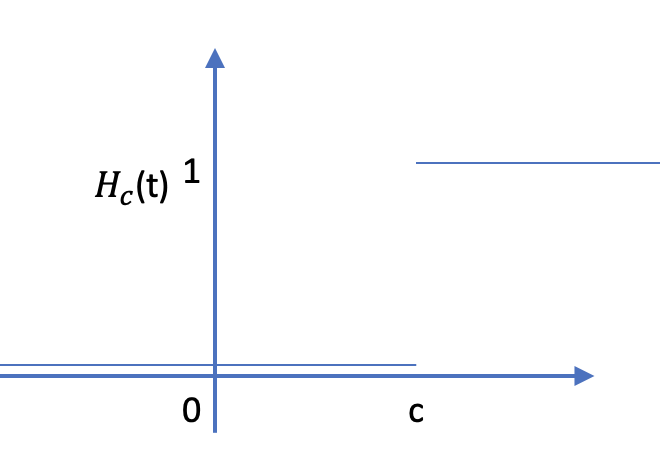
\includegraphics[width=6cm]{week9_2}
\end{figure}

\paragraph{lemma}
\[\lapl{H_c(t)f(t-c)}(s)=e^{-cs}F(s)\]
($F(s)=\lapl{f}(s)$)
\begin{figure}[H]
\centering
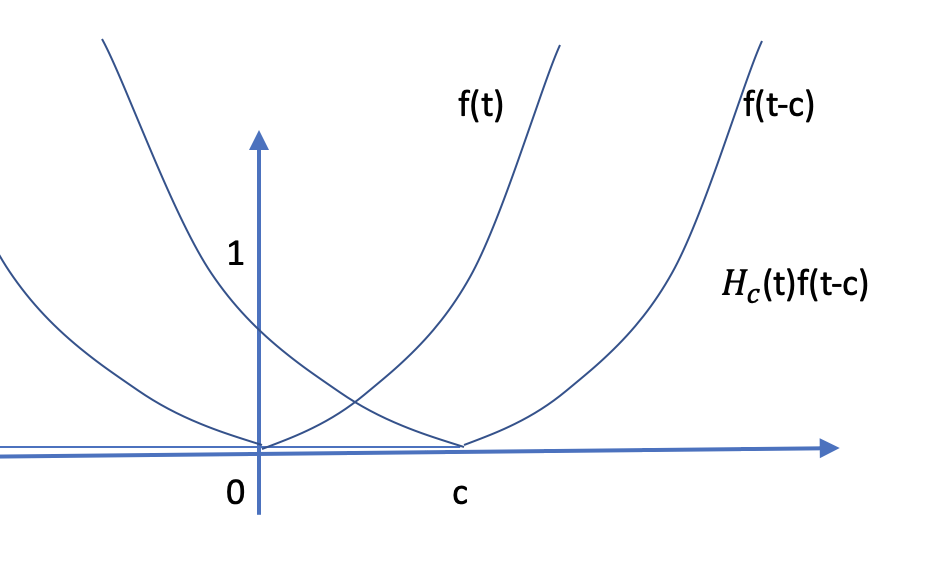
\includegraphics[width=8cm]{week9_3}
\end{figure}
\begin{proof}
\[\begin{aligned}
&\lapl{H_c(t)f(t-c)}(s)\\
=&\int_0^\infty e^{-st}H_c(t)f(t-c)\diff t\\
=&\int_c^\infty e^{-st}f(t-c)\diff t
\end{aligned}\]
$\bar{t}=t-c$
\[=\int_0^\infty e^{-s(\bar{t}+c)}f(\bar{t})\diff \bar{t}
\]
\[=\int_0^\infty e^{-s\bar{t}}f(\bar{t})\diff \bar{t} e^{-sc}
\]
\[=\lapl{f}(s)e^{-sc}
\]
\end{proof}
\begin{example}
\[y\pp-3y\p+2y=\begin{cases}\frac{1}{c},\quad 1<t<1+c\\0, \text{otherwise}\end{cases}
\]
\begin{figure}[H]
\centering
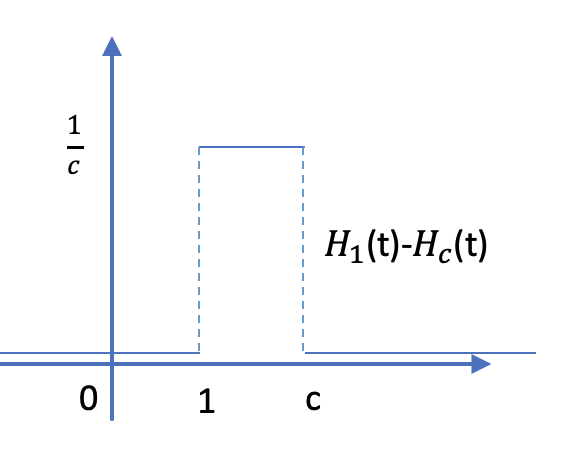
\includegraphics[width=6cm]{week9_4}
\end{figure}
\[Y=\lapl{y}\qquad y(0)=y\p(0)=0
\]
\[\begin{aligned}
&\lapl{y\pp-3y\p+2y}(s)\\
=&s^2Y(s)-3sY(s)+2Y(s)\\
=&Y(s)(s^2-3s+2)\dots(1)
\end{aligned}
\]
\[\begin{aligned}\lapl{\frac{1}{c}[H_1(t)-H_{1+c}(t)]}(s)&=\frac{1}{c}(\lapl{H_1(t)}(s)-\lapl{H_{1+c}(t)}(s))\\&=\frac{1}{c}(\frac{e^{-s}}{s}-\frac{e^{-(1+c)s}}{s})\dots(2)\end{aligned}
\]
(1)=(2), as we take laplace transformation on both side of the given equation in this example.
\[\begin{aligned}\therefore Y(s)&=\frac{\frac{1}{c}e^{-s}(1-e^{-cs})}{(s-1)(s-2)s}\\
&=\frac{1}{c}e^{-s}(1-e^{-cs})[\frac{1}{2s}-\frac{1}{s-1}+\frac{1}{2}\frac{1}{s-2}]\dots(3)\\
&=\frac{1}{c}e^{-s}(1-e^{-cs})\lapl{\frac{1}{2}-e^t+\frac{1}{2}e^{2t}}\dots(4)\\
&=\frac{1}{c}\lapl{H_1(t)[\frac{1}{2}-e^{t-1}+\frac{1}{2}e^{2(t-1)}]-H_{1+c}[\frac{1}{2}-e^{t-1-c}+\frac{1}{2}e^{2(t-1-c)}]}\dots(5)
\end{aligned}
\]
From (3) to (4), we do reverse laplace transformation, such as $\lapl{1}(s)=\int_0^\infty e^{-st}1\diff t=\dots=\frac{1}{s}$ and $\lapl{H_1(t)}(s)=e^{-s}\lapl{1}(s)$ (lemma above).\\
Procedure from (4) to (5) is due to lemma above.\\
Remember $Y(s)=\lapl{y}$
\[\begin{aligned}y(t)&=\frac{1}{c}\{H_1(t)[\frac{1}{2}-e^{t-1}+\frac{1}{2}e^{2(t-1)}]-H_{1+c}[\frac{1}{2}-e^{t-1-c}+\frac{1}{2}e^{2(t-1-c)}]\}\\
&=\frac{1}{c}\begin{cases}0,~t\leq1\\\frac{1}{2}-e^{t-1}+\frac{1}{2}e^{2(t-1)},~1<t<1+c\\-e^{t-1}+\frac{1}{2}e^{2(t-1)}+e^{t-1-c}-\frac{1}{2}e^{2(t-1-c)},~t\geq1+c\end{cases}
\end{aligned}
\]
As $c\rightarrow0$, $\frac{1}{2}e^{2(t-1)}\frac{1-e^{-2c}}{c}-e^{t-1}\frac{1-e^{-c}}{c}\rightarrow e^{2(t-1)}-e^{t-1}$ (by L'hospital's rule).

\end{example}

There is another way of doing this problem.
\begin{definition}[``Delta'' function: $\delta$] For any smooth function $\varphi$ with compact support on $\mathbb{R}$
\[\int_{-\infty}^\infty \delta(t)\varphi(t)\diff t=\varphi(0)
\]\end{definition}
\begin{example}[Example of delta function: ``Approximation to identity'']
A sequence of functions $\{\eta_\varepsilon\}$, $\eta(x)$ smooth supported inside $(-1,1)$, $\eta(-x)=\eta(x)\geq0$ and $\int_{-1}^1\eta(x)\diff x=1$\\
\[\eta(x)=\begin{cases}ce^{-\frac{1}{1-x^2}}~~|x|\leq1\\0~~|x|\geq1\end{cases}
\]
$c$ is chosen such that $\int_{-1}^1\eta=1$.
\[\eta_\varepsilon=\frac{1}{\varepsilon}\eta(\frac{x}{\varepsilon})
\]
 Want to show $\lim_{\varepsilon\rightarrow0}\eta_\varepsilon=\delta$, i.e. $\lim_{\varepsilon\rightarrow0}\int_{-\infty}^\infty\eta_\varepsilon(x)\varphi(x)\diff x=\varphi(0)$.
\end{example}
\begin{proof}
\[\int_{-\infty}^\infty\eta_\varepsilon(x)\diff x=1
\]
\[\begin{aligned}
|\int_{-\infty}^\infty\eta_\varepsilon(x)\varphi(x)\diff x-\varphi(0)|&=|\int_{-\infty}^\infty\eta_\varepsilon(x)\varphi(x)\diff x-\int_{-\infty}^\infty\eta_\varepsilon(x)\varphi(0)\diff x|\\
&\leq\int_{-\infty}^\infty|\eta_\varepsilon(x)[\varphi(x)-\varphi(0)]|\diff x=\int_{-\varepsilon}^\varepsilon\eta_\varepsilon(x)|\varphi(x)-\varphi(0)|\diff x\\
&\leq\int_{-\varepsilon}^\varepsilon\eta_{\varepsilon}(x)\diff x|\max_{|x|\leq\varepsilon}|\varphi(x)-\varphi(0)||\rightarrow0
\end{aligned}
\]




\end{proof}
\begin{remark}
Delta function isn't a function. As $\delta=\lim_{\varepsilon\rightarrow0}\eta_\varepsilon$, we can see delta function doesn't satisfy the definition of function at point 0. \\
In addition, the integral of delta function is equal to 1.

\end{remark}
\begin{example}
\[y\pp-3y\p+2y=\begin{cases}\frac{1}{c},~1<t<1+c\\0,~ \text{othrwise}\end{cases}
\]
\[y(0)=y\p(0)=0
\]
When $c\rightarrow0$, this question is the same as solve 
\[y\pp-3y\p+2y=\delta(t-1)
\]
\[Y(s)(s^2-3s+2)=\lapl{\delta(t-1)}(s)=\int_0^\infty e^{-st}\delta(t-1)\diff t
\]
\[\begin{aligned}
\therefore Y(s)&=\frac{e^{-s}}{(s-1)(s-2)}\\
&=e^{-s}(\frac{-1}{s-1}+\frac{1}{s-2})\\
&=\lapl{H_1(t)e^{t-1}+H_1(t)e^{2(t-1)}}(s)\\
&=\begin{cases}0,~t\leq1\\e^{2(t-1)}-e^{ct-1},~t\geq1\end{cases}
\end{aligned}
\]




\end{example}












\chapter{Week8}

\section{Monday}\index{Monday_lecture}
\subsection{Euler's Equation}
Recall previous knowledge,
\[t^2y\pp+\alpha ty\p+\beta y=0\qquad t>0
\]
$y=t^r$ $\Rightarrow\qquad$ $r(r-1)+\alpha r+\beta=0$ \\
$r^2+(\alpha-1)r+\beta=0$\\
$r_1,r_2=\frac{-(\alpha-1)\pm\sqrt{(\alpha-1)-4\beta}}{2}$
\begin{enumerate}
\item $(\alpha-1)^2-4\beta>0$  two real roots, $y=c_1t^{r_1}+c_2t^{r_2}$
\item $(\alpha-1)^2-4\beta=0$ $r_1=r_2=r$, $y=c_1t^r+c_2t^rlnt$
\item $(\alpha-1)^2-4\beta<0$ $r=\lambda\pm i\mu$, $y=t^\lambda[c_1\cos(\mu lnt)+c_2\sin(\mu lnt)]$
\end{enumerate}

Some motivations of Euler's Equation: Bessel's equation of order $\frac{1}{2}$\\
\[t^2y\pp+ty\p+(t^2-\frac{1}{4})y=0
\]
There doesn't exist a solution with the form of $y=\sum_{n=0}^\infty a_nt^n$. When $t=0$ it's a first order differential equation, the solution of this equation is only at one point $t=0$ which doesn't make much sense. We call this a singular point. We need to do something to factor out singularity.\\
\paragraph{Generalization}
\[L[y]\equiv t^2y\pp+t[p_0+p_1t+p_2t^2+\dots]y\p+[q_0+q_1t+q_2t^2+\dots]y=0
\]
Method of Frobenius,
\[y=\sum_{n=0}^\infty a_nt^{n+r}
\]
\begin{remark}
$r$ can be $\mathbb{R}$.\\
In order to avoid ambiguity, $a_0\neq 0$. Otherwise, it becomes $y=\sum_{n=1}^\infty a_nt^{n+r}$ which are the same as $y=\sum_{n=0}^{\infty}b_nt^{n+r\p}$. As $r$ and $r\p=r+1$ need to be determined, we have $y=\sum_{n=1}^\infty a_nt^{n+r}$ with the first term equals to zero, and $y=\sum_{n=0}^{\infty}b_nt^{n+r\p}$ to represent the same thing. Simply put, $a_0\neq 0$
\end{remark}
\[y\p=\sum_{n=0}^\infty(n+r)a_nt^{n+r-1}
\]
\[y\pp=\sum_{n=0}^{\infty}(n+r)(n+r-1)a_nt^{n+r-2}
\]
\[\begin{aligned}L[y]&=\sum_0^\infty(n+r)(n+r-1)a_nt^{n+r}+(\sum_{m=0}^\infty p_mt^m)(\sum_0^\infty (n+r)a_nt^{n+r})+\sum_{m=0}^\infty q_nt^m\sum_0^\infty a_nt^{n+r}\\
&=r(r-1)a_0+p_0ra_0+q_0a_0+[(1+r)ra_1+p_0(1+r)a_1+p_1ra_0+q_0a_1q_1a_0]t+\dots\\
&=[r(r-1)+p_0r+q_0]a_0+\underline{[\{(1+r)r+p_0(1+r)+q_0\}a_1+\{p_1r+q_1\}a_0]t}+\dots\\
&\quad+\underline{[(k+r)(k+r-1)a_k+\sum_{m=0}^kp_m(k-m+r)a_{k-m}+\sum_{n=0}^kq_ma_{k-m}]t^k}+\dots
\end{aligned}
\]
In order to have a solution $L[y]=0$,
Indicial equation
\[F(r)=r(r-1)+p_0r+q_0=0
\]
\[F(r+1)a_1=-[p_1r+q_1]a_0
\]
retrieved from first underline.\\Let's rewrite second underline a little bit.
\[=[(k+r)(k+r-1)a_k+\sum_0^{k-l}p_{k-l}(l+r)a_l+p_0a_k(k+r)+\sum_{n=1}^kq_{k-l}a_l+q_0a_k]t^k
\]
\[F(r+k)a_k=-[\sum_0^{k-1}\{p_{k-l}(l+1)+q_{k-l}\}a_l]
\]
It is clear that all $a_n$ can be solved recursively.\\
If there exists two real roots $r_1\geq r_2$, then 
\begin{itemize}
\item $r_1>r_2$ and $r_1-r_2$ is  not a positive integer. We will have two solutions.
\item $r_1>r_2$ and $r_1-r_2$ is a positive ineger then, you need to check textbook for more information as this will not be tested in the final.
\item $r_1=r_2$ check \textsection 2.8.3 for more information.
\end{itemize}
\begin{example}
\[t^2y\pp+ty\p+(-\frac{1}{4}+t^2)y=0
\]
$p_0=1$, $p_1=p_2=\dots=0$; $q=-\frac{1}{4}$, $q_1=0$, $q_2=1$, $q_3=0$\\Look at $L[y]\equiv t^2y\pp+t[p_0+p_1t+p_2t^2+\dots]y\p+[q_0+q_1t+q_2t^2+\dots]y=0$. You will know how we get all those stuffs.\\
$r(r-1)+r-\frac{1}{4}=0$, $r=\pm\frac{1}{2}$\\
First look at the first case $r=r_1=\frac{1}{2}$\\
$F(q+\frac{1}{2})a_1=0\Rightarrow a_1=0\dots(1)$ (We just pluge those stuffs in $F(r+1)a_1=-[p_1r+q_1]a_0$. \\
$F(k+r)a_k=k(k+1)a_k=-a_{k-2}\quad\Rightarrow ak=-\frac{1}{(k+1)ka_{k-2}}\dots(2)$  (As $F(k+r)=(r+k)^2-\frac{1}{4}=k(k+1)$)\\
With (1) and (2), we get $a_3=a_5=\dots=0$
\[a_2=-\frac{1}{3!}a_0
\]
\[a_4=-\frac{1}{5\cdot4}a_2=\frac{1}{5!}a_0
\]
\[a_{2n}=\frac{(-1)^n}{(2n+1)!}a_0
\]
\[y_1=a_0t^{\frac{1}{2}}(1-\frac{1}{3!}t^2+\frac{1}{5!}t^2-\dots)
\]
\[y_1=a_0t^{-\frac{1}{2}}\sin t
\]
$r_2=-\frac{1}{2}$
\[F(1+r_2)a_1=F(\frac{1}{2})a_1=0
\]
It's lucky both sides are equal to zero, else we cannot solve the second solution in this way.
\[F(k+r_2)=k(k-1)a_k=-q_2a_{k-2}=-a_{k-2}
\]
\[a_k=-\frac{1}{(k-1)k}a_{k-2}
\]
\[a_2=-\frac{1}{2}a_0
\]
\[a_4=-\frac{a_4}{4\cdot3}a_2=\frac{1}{4!}a_0
\]
\[a_6=-\frac{a_4}{6\cdot5}=-\frac{1}{6!}a_0
\]
\[y_2=t^{-\frac{1}{2}}a_0[1-\frac{1}{2!}t^2+\frac{1}{4!}t^4+\dots]=a_0t^{-\frac{1}{2}}\cos t
\]
Therefore, the general solutions is $y=\frac{1}{\sqrt{t}}(c_1\cos t+c_2\sin t)$
\end{example}



\section{Wednesday}\index{Wednesday_lecture}
\subsection{Laplace Transformation}
\[\lapl{f}(s)=\int_0^\infty e^{-st}f(t)\diff t
\]
\[|f(t)\leq Me^{ct}|\qquad\text{for t large, } s>c
\]
Heariside function $H(t)$
\begin{figure}[H]
\centering
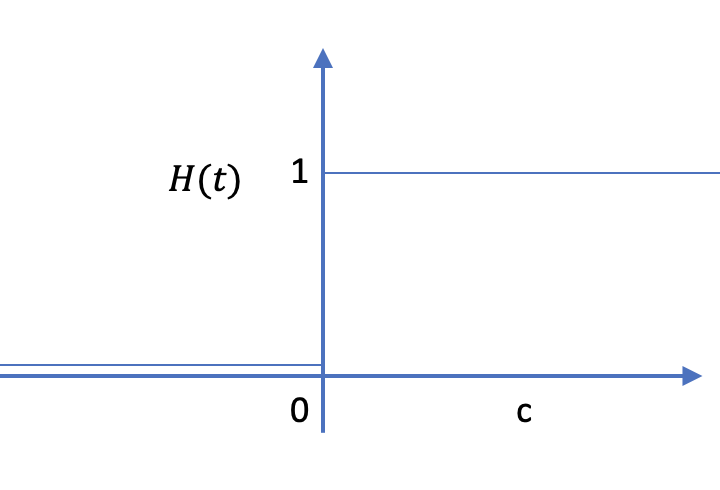
\includegraphics[width=6cm]{week9_1}
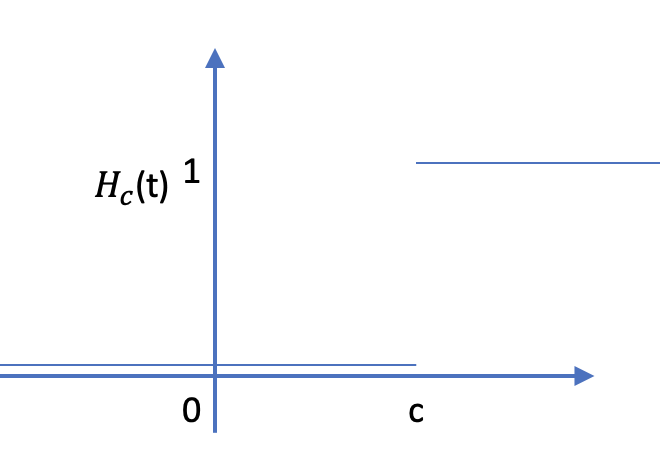
\includegraphics[width=6cm]{week9_2}
\end{figure}

\paragraph{lemma}
\[\lapl{H_c(t)f(t-c)}(s)=e^{-cs}F(s)\]
($F(s)=\lapl{f}(s)$)
\begin{figure}[H]
\centering
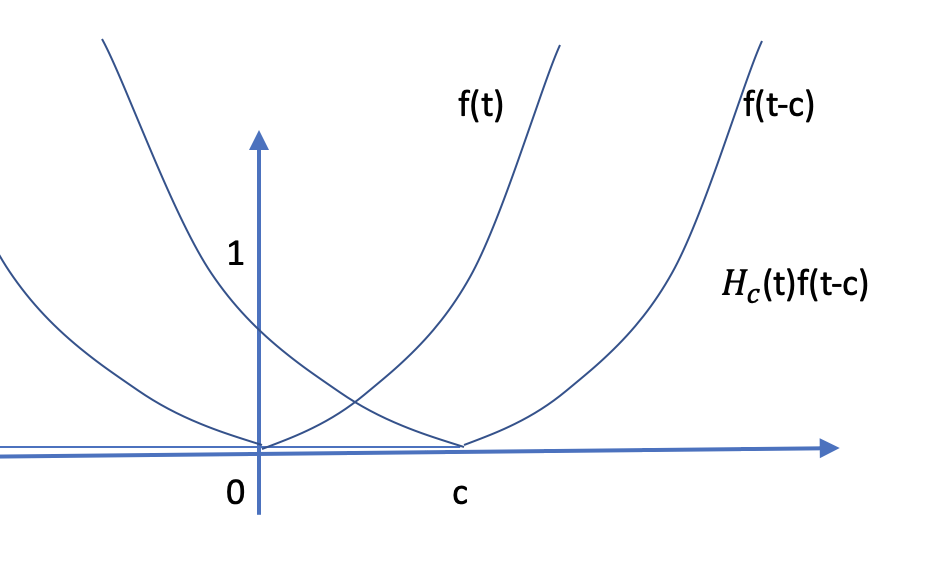
\includegraphics[width=8cm]{week9_3}
\end{figure}
\begin{proof}
\[\begin{aligned}
&\lapl{H_c(t)f(t-c)}(s)\\
=&\int_0^\infty e^{-st}H_c(t)f(t-c)\diff t\\
=&\int_c^\infty e^{-st}f(t-c)\diff t
\end{aligned}\]
$\bar{t}=t-c$
\[=\int_0^\infty e^{-s(\bar{t}+c)}f(\bar{t})\diff \bar{t}
\]
\[=\int_0^\infty e^{-s\bar{t}}f(\bar{t})\diff \bar{t} e^{-sc}
\]
\[=\lapl{f}(s)e^{-sc}
\]
\end{proof}
\begin{example}
\[y\pp-3y\p+2y=\begin{cases}\frac{1}{c},\quad 1<t<1+c\\0, \text{otherwise}\end{cases}
\]
\begin{figure}[H]
\centering
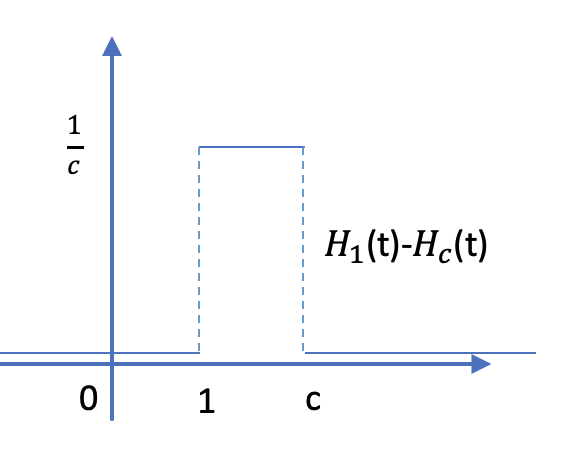
\includegraphics[width=6cm]{week9_4}
\end{figure}
\[Y=\lapl{y}\qquad y(0)=y\p(0)=0
\]
\[\begin{aligned}
&\lapl{y\pp-3y\p+2y}(s)\\
=&s^2Y(s)-3sY(s)+2Y(s)\\
=&Y(s)(s^2-3s+2)\dots(1)
\end{aligned}
\]
\[\begin{aligned}\lapl{\frac{1}{c}[H_1(t)-H_{1+c}(t)]}(s)&=\frac{1}{c}(\lapl{H_1(t)}(s)-\lapl{H_{1+c}(t)}(s))\\&=\frac{1}{c}(\frac{e^{-s}}{s}-\frac{e^{-(1+c)s}}{s})\dots(2)\end{aligned}
\]
(1)=(2), as we take laplace transformation on both side of the given equation in this example.
\[\begin{aligned}\therefore Y(s)&=\frac{\frac{1}{c}e^{-s}(1-e^{-cs})}{(s-1)(s-2)s}\\
&=\frac{1}{c}e^{-s}(1-e^{-cs})[\frac{1}{2s}-\frac{1}{s-1}+\frac{1}{2}\frac{1}{s-2}]\dots(3)\\
&=\frac{1}{c}e^{-s}(1-e^{-cs})\lapl{\frac{1}{2}-e^t+\frac{1}{2}e^{2t}}\dots(4)\\
&=\frac{1}{c}\lapl{H_1(t)[\frac{1}{2}-e^{t-1}+\frac{1}{2}e^{2(t-1)}]-H_{1+c}[\frac{1}{2}-e^{t-1-c}+\frac{1}{2}e^{2(t-1-c)}]}\dots(5)
\end{aligned}
\]
From (3) to (4), we do reverse laplace transformation, such as $\lapl{1}(s)=\int_0^\infty e^{-st}1\diff t=\dots=\frac{1}{s}$ and $\lapl{H_1(t)}(s)=e^{-s}\lapl{1}(s)$ (lemma above).\\
Procedure from (4) to (5) is due to lemma above.\\
Remember $Y(s)=\lapl{y}$
\[\begin{aligned}y(t)&=\frac{1}{c}\{H_1(t)[\frac{1}{2}-e^{t-1}+\frac{1}{2}e^{2(t-1)}]-H_{1+c}[\frac{1}{2}-e^{t-1-c}+\frac{1}{2}e^{2(t-1-c)}]\}\\
&=\frac{1}{c}\begin{cases}0,~t\leq1\\\frac{1}{2}-e^{t-1}+\frac{1}{2}e^{2(t-1)},~1<t<1+c\\-e^{t-1}+\frac{1}{2}e^{2(t-1)}+e^{t-1-c}-\frac{1}{2}e^{2(t-1-c)},~t\geq1+c\end{cases}
\end{aligned}
\]
As $c\rightarrow0$, $\frac{1}{2}e^{2(t-1)}\frac{1-e^{-2c}}{c}-e^{t-1}\frac{1-e^{-c}}{c}\rightarrow e^{2(t-1)}-e^{t-1}$ (by L'hospital's rule).

\end{example}

There is another way of doing this problem.
\begin{definition}[``Delta'' function: $\delta$] For any smooth function $\varphi$ with compact support on $\mathbb{R}$
\[\int_{-\infty}^\infty \delta(t)\varphi(t)\diff t=\varphi(0)
\]\end{definition}
\begin{example}[Example of delta function: ``Approximation to identity'']
A sequence of functions $\{\eta_\varepsilon\}$, $\eta(x)$ smooth supported inside $(-1,1)$, $\eta(-x)=\eta(x)\geq0$ and $\int_{-1}^1\eta(x)\diff x=1$\\
\[\eta(x)=\begin{cases}ce^{-\frac{1}{1-x^2}}~~|x|\leq1\\0~~|x|\geq1\end{cases}
\]
$c$ is chosen such that $\int_{-1}^1\eta=1$.
\[\eta_\varepsilon=\frac{1}{\varepsilon}\eta(\frac{x}{\varepsilon})
\]
 Want to show $\lim_{\varepsilon\rightarrow0}\eta_\varepsilon=\delta$, i.e. $\lim_{\varepsilon\rightarrow0}\int_{-\infty}^\infty\eta_\varepsilon(x)\varphi(x)\diff x=\varphi(0)$.
\end{example}
\begin{proof}
\[\int_{-\infty}^\infty\eta_\varepsilon(x)\diff x=1
\]
\[\begin{aligned}
|\int_{-\infty}^\infty\eta_\varepsilon(x)\varphi(x)\diff x-\varphi(0)|&=|\int_{-\infty}^\infty\eta_\varepsilon(x)\varphi(x)\diff x-\int_{-\infty}^\infty\eta_\varepsilon(x)\varphi(0)\diff x|\\
&\leq\int_{-\infty}^\infty|\eta_\varepsilon(x)[\varphi(x)-\varphi(0)]|\diff x=\int_{-\varepsilon}^\varepsilon\eta_\varepsilon(x)|\varphi(x)-\varphi(0)|\diff x\\
&\leq\int_{-\varepsilon}^\varepsilon\eta_{\varepsilon}(x)\diff x|\max_{|x|\leq\varepsilon}|\varphi(x)-\varphi(0)||\rightarrow0
\end{aligned}
\]




\end{proof}
\begin{remark}
Delta function isn't a function. As $\delta=\lim_{\varepsilon\rightarrow0}\eta_\varepsilon$, we can see delta function doesn't satisfy the definition of function at point 0. \\
In addition, the integral of delta function is equal to 1.

\end{remark}
\begin{example}
\[y\pp-3y\p+2y=\begin{cases}\frac{1}{c},~1<t<1+c\\0,~ \text{othrwise}\end{cases}
\]
\[y(0)=y\p(0)=0
\]
When $c\rightarrow0$, this question is the same as solve 
\[y\pp-3y\p+2y=\delta(t-1)
\]
\[Y(s)(s^2-3s+2)=\lapl{\delta(t-1)}(s)=\int_0^\infty e^{-st}\delta(t-1)\diff t
\]
\[\begin{aligned}
\therefore Y(s)&=\frac{e^{-s}}{(s-1)(s-2)}\\
&=e^{-s}(\frac{-1}{s-1}+\frac{1}{s-2})\\
&=\lapl{H_1(t)e^{t-1}+H_1(t)e^{2(t-1)}}(s)\\
&=\begin{cases}0,~t\leq1\\e^{2(t-1)}-e^{ct-1},~t\geq1\end{cases}
\end{aligned}
\]




\end{example}












\chapter{Week8}

\section{Monday}\index{Monday_lecture}
\subsection{Euler's Equation}
Recall previous knowledge,
\[t^2y\pp+\alpha ty\p+\beta y=0\qquad t>0
\]
$y=t^r$ $\Rightarrow\qquad$ $r(r-1)+\alpha r+\beta=0$ \\
$r^2+(\alpha-1)r+\beta=0$\\
$r_1,r_2=\frac{-(\alpha-1)\pm\sqrt{(\alpha-1)-4\beta}}{2}$
\begin{enumerate}
\item $(\alpha-1)^2-4\beta>0$  two real roots, $y=c_1t^{r_1}+c_2t^{r_2}$
\item $(\alpha-1)^2-4\beta=0$ $r_1=r_2=r$, $y=c_1t^r+c_2t^rlnt$
\item $(\alpha-1)^2-4\beta<0$ $r=\lambda\pm i\mu$, $y=t^\lambda[c_1\cos(\mu lnt)+c_2\sin(\mu lnt)]$
\end{enumerate}

Some motivations of Euler's Equation: Bessel's equation of order $\frac{1}{2}$\\
\[t^2y\pp+ty\p+(t^2-\frac{1}{4})y=0
\]
There doesn't exist a solution with the form of $y=\sum_{n=0}^\infty a_nt^n$. When $t=0$ it's a first order differential equation, the solution of this equation is only at one point $t=0$ which doesn't make much sense. We call this a singular point. We need to do something to factor out singularity.\\
\paragraph{Generalization}
\[L[y]\equiv t^2y\pp+t[p_0+p_1t+p_2t^2+\dots]y\p+[q_0+q_1t+q_2t^2+\dots]y=0
\]
Method of Frobenius,
\[y=\sum_{n=0}^\infty a_nt^{n+r}
\]
\begin{remark}
$r$ can be $\mathbb{R}$.\\
In order to avoid ambiguity, $a_0\neq 0$. Otherwise, it becomes $y=\sum_{n=1}^\infty a_nt^{n+r}$ which are the same as $y=\sum_{n=0}^{\infty}b_nt^{n+r\p}$. As $r$ and $r\p=r+1$ need to be determined, we have $y=\sum_{n=1}^\infty a_nt^{n+r}$ with the first term equals to zero, and $y=\sum_{n=0}^{\infty}b_nt^{n+r\p}$ to represent the same thing. Simply put, $a_0\neq 0$
\end{remark}
\[y\p=\sum_{n=0}^\infty(n+r)a_nt^{n+r-1}
\]
\[y\pp=\sum_{n=0}^{\infty}(n+r)(n+r-1)a_nt^{n+r-2}
\]
\[\begin{aligned}L[y]&=\sum_0^\infty(n+r)(n+r-1)a_nt^{n+r}+(\sum_{m=0}^\infty p_mt^m)(\sum_0^\infty (n+r)a_nt^{n+r})+\sum_{m=0}^\infty q_nt^m\sum_0^\infty a_nt^{n+r}\\
&=r(r-1)a_0+p_0ra_0+q_0a_0+[(1+r)ra_1+p_0(1+r)a_1+p_1ra_0+q_0a_1q_1a_0]t+\dots\\
&=[r(r-1)+p_0r+q_0]a_0+\underline{[\{(1+r)r+p_0(1+r)+q_0\}a_1+\{p_1r+q_1\}a_0]t}+\dots\\
&\quad+\underline{[(k+r)(k+r-1)a_k+\sum_{m=0}^kp_m(k-m+r)a_{k-m}+\sum_{n=0}^kq_ma_{k-m}]t^k}+\dots
\end{aligned}
\]
In order to have a solution $L[y]=0$,
Indicial equation
\[F(r)=r(r-1)+p_0r+q_0=0
\]
\[F(r+1)a_1=-[p_1r+q_1]a_0
\]
retrieved from first underline.\\Let's rewrite second underline a little bit.
\[=[(k+r)(k+r-1)a_k+\sum_0^{k-l}p_{k-l}(l+r)a_l+p_0a_k(k+r)+\sum_{n=1}^kq_{k-l}a_l+q_0a_k]t^k
\]
\[F(r+k)a_k=-[\sum_0^{k-1}\{p_{k-l}(l+1)+q_{k-l}\}a_l]
\]
It is clear that all $a_n$ can be solved recursively.\\
If there exists two real roots $r_1\geq r_2$, then 
\begin{itemize}
\item $r_1>r_2$ and $r_1-r_2$ is  not a positive integer. We will have two solutions.
\item $r_1>r_2$ and $r_1-r_2$ is a positive ineger then, you need to check textbook for more information as this will not be tested in the final.
\item $r_1=r_2$ check \textsection 2.8.3 for more information.
\end{itemize}
\begin{example}
\[t^2y\pp+ty\p+(-\frac{1}{4}+t^2)y=0
\]
$p_0=1$, $p_1=p_2=\dots=0$; $q=-\frac{1}{4}$, $q_1=0$, $q_2=1$, $q_3=0$\\Look at $L[y]\equiv t^2y\pp+t[p_0+p_1t+p_2t^2+\dots]y\p+[q_0+q_1t+q_2t^2+\dots]y=0$. You will know how we get all those stuffs.\\
$r(r-1)+r-\frac{1}{4}=0$, $r=\pm\frac{1}{2}$\\
First look at the first case $r=r_1=\frac{1}{2}$\\
$F(q+\frac{1}{2})a_1=0\Rightarrow a_1=0\dots(1)$ (We just pluge those stuffs in $F(r+1)a_1=-[p_1r+q_1]a_0$. \\
$F(k+r)a_k=k(k+1)a_k=-a_{k-2}\quad\Rightarrow ak=-\frac{1}{(k+1)ka_{k-2}}\dots(2)$  (As $F(k+r)=(r+k)^2-\frac{1}{4}=k(k+1)$)\\
With (1) and (2), we get $a_3=a_5=\dots=0$
\[a_2=-\frac{1}{3!}a_0
\]
\[a_4=-\frac{1}{5\cdot4}a_2=\frac{1}{5!}a_0
\]
\[a_{2n}=\frac{(-1)^n}{(2n+1)!}a_0
\]
\[y_1=a_0t^{\frac{1}{2}}(1-\frac{1}{3!}t^2+\frac{1}{5!}t^2-\dots)
\]
\[y_1=a_0t^{-\frac{1}{2}}\sin t
\]
$r_2=-\frac{1}{2}$
\[F(1+r_2)a_1=F(\frac{1}{2})a_1=0
\]
It's lucky both sides are equal to zero, else we cannot solve the second solution in this way.
\[F(k+r_2)=k(k-1)a_k=-q_2a_{k-2}=-a_{k-2}
\]
\[a_k=-\frac{1}{(k-1)k}a_{k-2}
\]
\[a_2=-\frac{1}{2}a_0
\]
\[a_4=-\frac{a_4}{4\cdot3}a_2=\frac{1}{4!}a_0
\]
\[a_6=-\frac{a_4}{6\cdot5}=-\frac{1}{6!}a_0
\]
\[y_2=t^{-\frac{1}{2}}a_0[1-\frac{1}{2!}t^2+\frac{1}{4!}t^4+\dots]=a_0t^{-\frac{1}{2}}\cos t
\]
Therefore, the general solutions is $y=\frac{1}{\sqrt{t}}(c_1\cos t+c_2\sin t)$
\end{example}



\section{Wednesday}\index{Wednesday_lecture}
\subsection{Application}
\paragraph{Mixture problem}There are two things that you need to bear in mind: \\\textcolor{red}{$\frac{\diff y}{\diff t}=$ input rate - output rate}, carry the units.

\begin{example}
A 120-gal tank initially contain 90kg salt dissoved in 90-gal of water. Brine containing 2kg/gal of salt flows into the tank at the water. Brine containing 2kg/gal of salt flows into the tank at the rate of 4gal/min, \& the well-stirned mixture flows out at the rate of 3 gal/min. How much salt does the tank contain when it is full?
\begin{figure}[H]
\centering
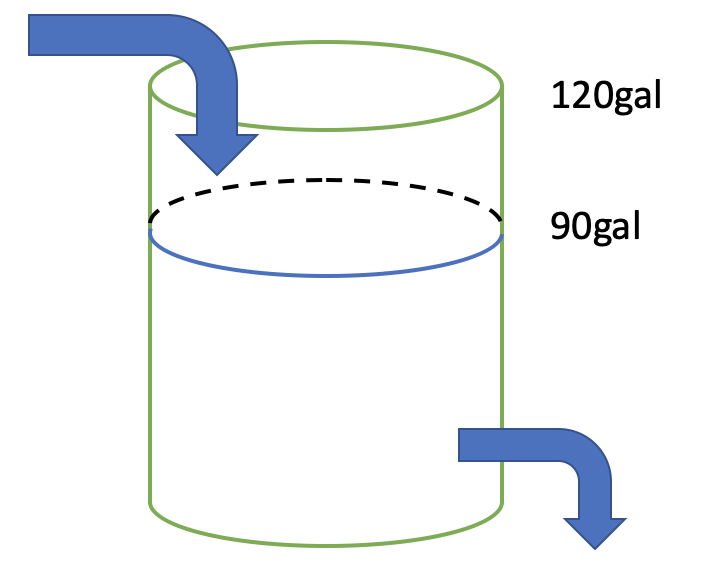
\includegraphics[width=5cm]{week2_wed_first}
\caption{First}
\end{figure}
Set $y(t)=$ the amount of salt at time $t$,\\ $V(t)=$the amount of brine at time $t$= 90 +$t$(gal)(t:minute)\\
\[\begin{aligned}y^\prime(t)&=2\text{kg/gal}\cdotp4\text{gal/min}-\frac{y(t)}{V(t)}\text{kg/gal}\cdotp3\text{gal/min}\\
&=8\text{kg/min}-3\frac{y(t)}{V(t)}\text{kg/min}
\end{aligned}
\]
\[y^\prime=8-3\frac{y}{90+t}
\]
\[y^\prime+\frac{3}{90+t}y=8
\]
By intergrating factor,
\[(e^{\int\frac{3}{90+t}\diff t}\cdotp y)^\prime=8e^{\int\frac{3}{90+t}\diff t}
\]
Try to simplify $e^{\int\frac{3}{90+t}\diff t}$;
\[\begin{aligned}\int\frac{3}{90+t}\diff t&=3ln|90+t|+\tilde{c}\\&=3ln(90+t)+\tilde{c}\end{aligned}
\]
Then,
\[e^{\int\frac{3}{90+t}\diff t}=(90+t)^3\cdotp c
\]
Integrate both sides,
\[(90+t)^3\cdotp c\cdotp y=8\int(90+t)^3\cdotp c\diff t
\]
\[(90+t)^3y=2\cdotp(90+t)^4+C
\]
\[y=2(90+t)+\frac{c}{(90+t)^3}
\]
\[y(0)=90=180+\frac{c}{90^3}\quad\Rightarrow\quad c=-90^4
\]
\[y=2(90+t)-\frac{90^4}{(90+t)^3}
\]
At $t=30$ the tank is full \& $y(30)=240-\frac{90^3}{120^3}\cdotp90$
\end{example}

\begin{example}[Persuit problem]
In a naval excercise, a distroyler $D$ is hunting a submarine $S$. Suppose $D$ at $(9,0)$ detects $S$ at $(0,0)$ \& at the same time $S$ detects $D$. Assuming that $S$ will dive immediately \& depart at full speed, $15$mile/hr in a straight course of unknown direction. What path should the destroyer $D$ follows to be certain of passing directly over the submarine $S$. If the speed of $D$ is $30$mile/hr at all time of the pursuit?
\begin{figure}[H]
\centering
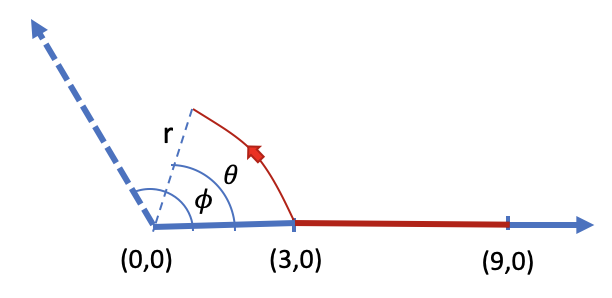
\includegraphics[width=8cm]{week2_wed_sec}
\caption{The path of destroyler in red.}
\end{figure}
Distance $D$ has travelled=$6+\int_0^\phi\sqrt{(r(\theta))^2+(r^\prime(\theta))^2}\diff\theta$.\\
Distance $S$ has travelled=$r(\phi)$.\\
For the speed of $D$ is twice than that of $S$, with the same period of time:
\[6+\int_0^\phi\sqrt{(r(\theta))^2+(r^\prime(\theta))^2}\diff\theta=2r(\phi)
\]
This isn't a form that can be dealt with. Differentiate both side,
\[\sqrt{(r(\phi))^2+(r^\prime(\phi))^2}=2r^\prime(\phi)
\]
\[(r(\phi))^2+(r^\prime(\phi))^2=4(r^\prime(\phi))^2
\]
\[r^\prime(\phi)=\pm\frac{1}{\sqrt{3}}r(\phi)
\]
W.L.O.G pick plus sign $\frac{r^\prime}{r}=\frac{1}{\sqrt{3}}$
\[lnr=\frac{1}{\sqrt{3}}\phi+\tilde{c}
\]
\[r=e^{\frac{\phi}{\sqrt{3}}}\cdotp c
\]
\[r(0)=3=c
\]
\[r(\phi)=3e^{\frac{\phi}{\sqrt{3}}}
\]
Given the direction $S$ take $\phi$, if $D$ want to be above it, they would reach each other at $(\phi,3e^{\frac{\phi}{\sqrt{3}}})$. This implies that if $D$ follows the path of 
$r(\theta)=3e^{\frac{\theta}{\sqrt{3}}}$, $D$ can catch $S$ whichever direction $S$ take.
\end{example}
\begin{remark}
There is a link about basic idea of how to compute the length of a curve:
\href{http://tutorial.math.lamar.edu/Classes/CalcII/ArcLength.aspx}{http://tutorial.math.lamar.edu/Classes/CalcII/ArcLength.aspx}. Check it if you are interested.
\end{remark}
\paragraph{Orthoganal trajectories} Given a family of curve $f(x,y,c)=0$. To find its orthoganal trajectories, the slope of the graph is needed. Differentiate $F$ by $x$;
\[F_x+F_yy_x=0
\]
Slope is $y_x=-\frac{F_x}{F_y}$. Then the slope of the graph that is orthoganal to the original one is \[y_x=\frac{F_y}{F_x}=\frac{\frac{\partial F}{\partial y}(x,y,c)}{\frac{\partial F}{\partial x}(x,y,c)}\]
\begin{example}
$y=cx^2$ $c$:parameter. To find another family of curves which is orthoganal to $y=cx^2$ whenever they intersect with each other.\\
$y=cx^2$, $\frac{\diff f}{\diff x}=2cx$ O.T. $\rightarrow \frac{\diff f}{\diff x}=\frac{-1}{2cx}=\frac{-1}{2\frac{y}{x^2}x}=-\frac{x}{2y}$ ( A separable equation)\\
$2y\diff y+x\diff x=0\quad\rightarrow\quad y^2+\frac{1}{2}x^2=c$
\end{example}



\chapter{Week8}

\section{Monday}\index{Monday_lecture}
\subsection{Euler's Equation}
Recall previous knowledge,
\[t^2y\pp+\alpha ty\p+\beta y=0\qquad t>0
\]
$y=t^r$ $\Rightarrow\qquad$ $r(r-1)+\alpha r+\beta=0$ \\
$r^2+(\alpha-1)r+\beta=0$\\
$r_1,r_2=\frac{-(\alpha-1)\pm\sqrt{(\alpha-1)-4\beta}}{2}$
\begin{enumerate}
\item $(\alpha-1)^2-4\beta>0$  two real roots, $y=c_1t^{r_1}+c_2t^{r_2}$
\item $(\alpha-1)^2-4\beta=0$ $r_1=r_2=r$, $y=c_1t^r+c_2t^rlnt$
\item $(\alpha-1)^2-4\beta<0$ $r=\lambda\pm i\mu$, $y=t^\lambda[c_1\cos(\mu lnt)+c_2\sin(\mu lnt)]$
\end{enumerate}

Some motivations of Euler's Equation: Bessel's equation of order $\frac{1}{2}$\\
\[t^2y\pp+ty\p+(t^2-\frac{1}{4})y=0
\]
There doesn't exist a solution with the form of $y=\sum_{n=0}^\infty a_nt^n$. When $t=0$ it's a first order differential equation, the solution of this equation is only at one point $t=0$ which doesn't make much sense. We call this a singular point. We need to do something to factor out singularity.\\
\paragraph{Generalization}
\[L[y]\equiv t^2y\pp+t[p_0+p_1t+p_2t^2+\dots]y\p+[q_0+q_1t+q_2t^2+\dots]y=0
\]
Method of Frobenius,
\[y=\sum_{n=0}^\infty a_nt^{n+r}
\]
\begin{remark}
$r$ can be $\mathbb{R}$.\\
In order to avoid ambiguity, $a_0\neq 0$. Otherwise, it becomes $y=\sum_{n=1}^\infty a_nt^{n+r}$ which are the same as $y=\sum_{n=0}^{\infty}b_nt^{n+r\p}$. As $r$ and $r\p=r+1$ need to be determined, we have $y=\sum_{n=1}^\infty a_nt^{n+r}$ with the first term equals to zero, and $y=\sum_{n=0}^{\infty}b_nt^{n+r\p}$ to represent the same thing. Simply put, $a_0\neq 0$
\end{remark}
\[y\p=\sum_{n=0}^\infty(n+r)a_nt^{n+r-1}
\]
\[y\pp=\sum_{n=0}^{\infty}(n+r)(n+r-1)a_nt^{n+r-2}
\]
\[\begin{aligned}L[y]&=\sum_0^\infty(n+r)(n+r-1)a_nt^{n+r}+(\sum_{m=0}^\infty p_mt^m)(\sum_0^\infty (n+r)a_nt^{n+r})+\sum_{m=0}^\infty q_nt^m\sum_0^\infty a_nt^{n+r}\\
&=r(r-1)a_0+p_0ra_0+q_0a_0+[(1+r)ra_1+p_0(1+r)a_1+p_1ra_0+q_0a_1q_1a_0]t+\dots\\
&=[r(r-1)+p_0r+q_0]a_0+\underline{[\{(1+r)r+p_0(1+r)+q_0\}a_1+\{p_1r+q_1\}a_0]t}+\dots\\
&\quad+\underline{[(k+r)(k+r-1)a_k+\sum_{m=0}^kp_m(k-m+r)a_{k-m}+\sum_{n=0}^kq_ma_{k-m}]t^k}+\dots
\end{aligned}
\]
In order to have a solution $L[y]=0$,
Indicial equation
\[F(r)=r(r-1)+p_0r+q_0=0
\]
\[F(r+1)a_1=-[p_1r+q_1]a_0
\]
retrieved from first underline.\\Let's rewrite second underline a little bit.
\[=[(k+r)(k+r-1)a_k+\sum_0^{k-l}p_{k-l}(l+r)a_l+p_0a_k(k+r)+\sum_{n=1}^kq_{k-l}a_l+q_0a_k]t^k
\]
\[F(r+k)a_k=-[\sum_0^{k-1}\{p_{k-l}(l+1)+q_{k-l}\}a_l]
\]
It is clear that all $a_n$ can be solved recursively.\\
If there exists two real roots $r_1\geq r_2$, then 
\begin{itemize}
\item $r_1>r_2$ and $r_1-r_2$ is  not a positive integer. We will have two solutions.
\item $r_1>r_2$ and $r_1-r_2$ is a positive ineger then, you need to check textbook for more information as this will not be tested in the final.
\item $r_1=r_2$ check \textsection 2.8.3 for more information.
\end{itemize}
\begin{example}
\[t^2y\pp+ty\p+(-\frac{1}{4}+t^2)y=0
\]
$p_0=1$, $p_1=p_2=\dots=0$; $q=-\frac{1}{4}$, $q_1=0$, $q_2=1$, $q_3=0$\\Look at $L[y]\equiv t^2y\pp+t[p_0+p_1t+p_2t^2+\dots]y\p+[q_0+q_1t+q_2t^2+\dots]y=0$. You will know how we get all those stuffs.\\
$r(r-1)+r-\frac{1}{4}=0$, $r=\pm\frac{1}{2}$\\
First look at the first case $r=r_1=\frac{1}{2}$\\
$F(q+\frac{1}{2})a_1=0\Rightarrow a_1=0\dots(1)$ (We just pluge those stuffs in $F(r+1)a_1=-[p_1r+q_1]a_0$. \\
$F(k+r)a_k=k(k+1)a_k=-a_{k-2}\quad\Rightarrow ak=-\frac{1}{(k+1)ka_{k-2}}\dots(2)$  (As $F(k+r)=(r+k)^2-\frac{1}{4}=k(k+1)$)\\
With (1) and (2), we get $a_3=a_5=\dots=0$
\[a_2=-\frac{1}{3!}a_0
\]
\[a_4=-\frac{1}{5\cdot4}a_2=\frac{1}{5!}a_0
\]
\[a_{2n}=\frac{(-1)^n}{(2n+1)!}a_0
\]
\[y_1=a_0t^{\frac{1}{2}}(1-\frac{1}{3!}t^2+\frac{1}{5!}t^2-\dots)
\]
\[y_1=a_0t^{-\frac{1}{2}}\sin t
\]
$r_2=-\frac{1}{2}$
\[F(1+r_2)a_1=F(\frac{1}{2})a_1=0
\]
It's lucky both sides are equal to zero, else we cannot solve the second solution in this way.
\[F(k+r_2)=k(k-1)a_k=-q_2a_{k-2}=-a_{k-2}
\]
\[a_k=-\frac{1}{(k-1)k}a_{k-2}
\]
\[a_2=-\frac{1}{2}a_0
\]
\[a_4=-\frac{a_4}{4\cdot3}a_2=\frac{1}{4!}a_0
\]
\[a_6=-\frac{a_4}{6\cdot5}=-\frac{1}{6!}a_0
\]
\[y_2=t^{-\frac{1}{2}}a_0[1-\frac{1}{2!}t^2+\frac{1}{4!}t^4+\dots]=a_0t^{-\frac{1}{2}}\cos t
\]
Therefore, the general solutions is $y=\frac{1}{\sqrt{t}}(c_1\cos t+c_2\sin t)$
\end{example}


\chapter{Week8}

\section{Monday}\index{Monday_lecture}
\subsection{Euler's Equation}
Recall previous knowledge,
\[t^2y\pp+\alpha ty\p+\beta y=0\qquad t>0
\]
$y=t^r$ $\Rightarrow\qquad$ $r(r-1)+\alpha r+\beta=0$ \\
$r^2+(\alpha-1)r+\beta=0$\\
$r_1,r_2=\frac{-(\alpha-1)\pm\sqrt{(\alpha-1)-4\beta}}{2}$
\begin{enumerate}
\item $(\alpha-1)^2-4\beta>0$  two real roots, $y=c_1t^{r_1}+c_2t^{r_2}$
\item $(\alpha-1)^2-4\beta=0$ $r_1=r_2=r$, $y=c_1t^r+c_2t^rlnt$
\item $(\alpha-1)^2-4\beta<0$ $r=\lambda\pm i\mu$, $y=t^\lambda[c_1\cos(\mu lnt)+c_2\sin(\mu lnt)]$
\end{enumerate}

Some motivations of Euler's Equation: Bessel's equation of order $\frac{1}{2}$\\
\[t^2y\pp+ty\p+(t^2-\frac{1}{4})y=0
\]
There doesn't exist a solution with the form of $y=\sum_{n=0}^\infty a_nt^n$. When $t=0$ it's a first order differential equation, the solution of this equation is only at one point $t=0$ which doesn't make much sense. We call this a singular point. We need to do something to factor out singularity.\\
\paragraph{Generalization}
\[L[y]\equiv t^2y\pp+t[p_0+p_1t+p_2t^2+\dots]y\p+[q_0+q_1t+q_2t^2+\dots]y=0
\]
Method of Frobenius,
\[y=\sum_{n=0}^\infty a_nt^{n+r}
\]
\begin{remark}
$r$ can be $\mathbb{R}$.\\
In order to avoid ambiguity, $a_0\neq 0$. Otherwise, it becomes $y=\sum_{n=1}^\infty a_nt^{n+r}$ which are the same as $y=\sum_{n=0}^{\infty}b_nt^{n+r\p}$. As $r$ and $r\p=r+1$ need to be determined, we have $y=\sum_{n=1}^\infty a_nt^{n+r}$ with the first term equals to zero, and $y=\sum_{n=0}^{\infty}b_nt^{n+r\p}$ to represent the same thing. Simply put, $a_0\neq 0$
\end{remark}
\[y\p=\sum_{n=0}^\infty(n+r)a_nt^{n+r-1}
\]
\[y\pp=\sum_{n=0}^{\infty}(n+r)(n+r-1)a_nt^{n+r-2}
\]
\[\begin{aligned}L[y]&=\sum_0^\infty(n+r)(n+r-1)a_nt^{n+r}+(\sum_{m=0}^\infty p_mt^m)(\sum_0^\infty (n+r)a_nt^{n+r})+\sum_{m=0}^\infty q_nt^m\sum_0^\infty a_nt^{n+r}\\
&=r(r-1)a_0+p_0ra_0+q_0a_0+[(1+r)ra_1+p_0(1+r)a_1+p_1ra_0+q_0a_1q_1a_0]t+\dots\\
&=[r(r-1)+p_0r+q_0]a_0+\underline{[\{(1+r)r+p_0(1+r)+q_0\}a_1+\{p_1r+q_1\}a_0]t}+\dots\\
&\quad+\underline{[(k+r)(k+r-1)a_k+\sum_{m=0}^kp_m(k-m+r)a_{k-m}+\sum_{n=0}^kq_ma_{k-m}]t^k}+\dots
\end{aligned}
\]
In order to have a solution $L[y]=0$,
Indicial equation
\[F(r)=r(r-1)+p_0r+q_0=0
\]
\[F(r+1)a_1=-[p_1r+q_1]a_0
\]
retrieved from first underline.\\Let's rewrite second underline a little bit.
\[=[(k+r)(k+r-1)a_k+\sum_0^{k-l}p_{k-l}(l+r)a_l+p_0a_k(k+r)+\sum_{n=1}^kq_{k-l}a_l+q_0a_k]t^k
\]
\[F(r+k)a_k=-[\sum_0^{k-1}\{p_{k-l}(l+1)+q_{k-l}\}a_l]
\]
It is clear that all $a_n$ can be solved recursively.\\
If there exists two real roots $r_1\geq r_2$, then 
\begin{itemize}
\item $r_1>r_2$ and $r_1-r_2$ is  not a positive integer. We will have two solutions.
\item $r_1>r_2$ and $r_1-r_2$ is a positive ineger then, you need to check textbook for more information as this will not be tested in the final.
\item $r_1=r_2$ check \textsection 2.8.3 for more information.
\end{itemize}
\begin{example}
\[t^2y\pp+ty\p+(-\frac{1}{4}+t^2)y=0
\]
$p_0=1$, $p_1=p_2=\dots=0$; $q=-\frac{1}{4}$, $q_1=0$, $q_2=1$, $q_3=0$\\Look at $L[y]\equiv t^2y\pp+t[p_0+p_1t+p_2t^2+\dots]y\p+[q_0+q_1t+q_2t^2+\dots]y=0$. You will know how we get all those stuffs.\\
$r(r-1)+r-\frac{1}{4}=0$, $r=\pm\frac{1}{2}$\\
First look at the first case $r=r_1=\frac{1}{2}$\\
$F(q+\frac{1}{2})a_1=0\Rightarrow a_1=0\dots(1)$ (We just pluge those stuffs in $F(r+1)a_1=-[p_1r+q_1]a_0$. \\
$F(k+r)a_k=k(k+1)a_k=-a_{k-2}\quad\Rightarrow ak=-\frac{1}{(k+1)ka_{k-2}}\dots(2)$  (As $F(k+r)=(r+k)^2-\frac{1}{4}=k(k+1)$)\\
With (1) and (2), we get $a_3=a_5=\dots=0$
\[a_2=-\frac{1}{3!}a_0
\]
\[a_4=-\frac{1}{5\cdot4}a_2=\frac{1}{5!}a_0
\]
\[a_{2n}=\frac{(-1)^n}{(2n+1)!}a_0
\]
\[y_1=a_0t^{\frac{1}{2}}(1-\frac{1}{3!}t^2+\frac{1}{5!}t^2-\dots)
\]
\[y_1=a_0t^{-\frac{1}{2}}\sin t
\]
$r_2=-\frac{1}{2}$
\[F(1+r_2)a_1=F(\frac{1}{2})a_1=0
\]
It's lucky both sides are equal to zero, else we cannot solve the second solution in this way.
\[F(k+r_2)=k(k-1)a_k=-q_2a_{k-2}=-a_{k-2}
\]
\[a_k=-\frac{1}{(k-1)k}a_{k-2}
\]
\[a_2=-\frac{1}{2}a_0
\]
\[a_4=-\frac{a_4}{4\cdot3}a_2=\frac{1}{4!}a_0
\]
\[a_6=-\frac{a_4}{6\cdot5}=-\frac{1}{6!}a_0
\]
\[y_2=t^{-\frac{1}{2}}a_0[1-\frac{1}{2!}t^2+\frac{1}{4!}t^4+\dots]=a_0t^{-\frac{1}{2}}\cos t
\]
Therefore, the general solutions is $y=\frac{1}{\sqrt{t}}(c_1\cos t+c_2\sin t)$
\end{example}



\section{Wednesday}\index{Wednesday_lecture}
\subsection{Laplace Transformation}
\[\lapl{f}(s)=\int_0^\infty e^{-st}f(t)\diff t
\]
\[|f(t)\leq Me^{ct}|\qquad\text{for t large, } s>c
\]
Heariside function $H(t)$
\begin{figure}[H]
\centering
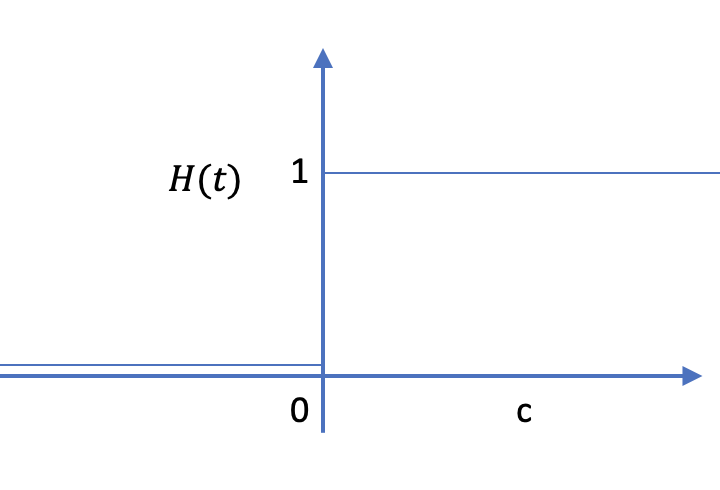
\includegraphics[width=6cm]{week9_1}
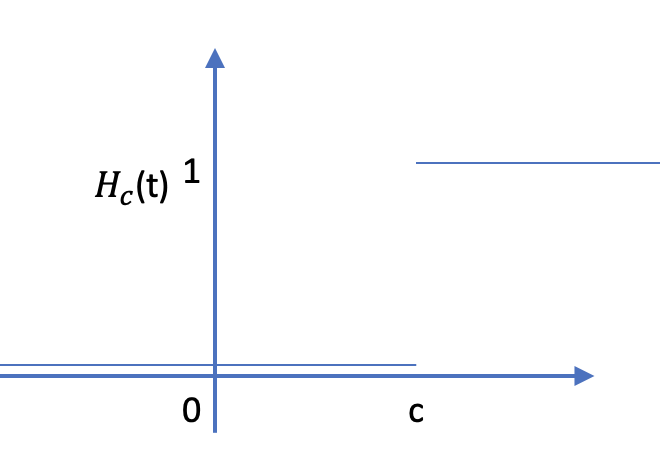
\includegraphics[width=6cm]{week9_2}
\end{figure}

\paragraph{lemma}
\[\lapl{H_c(t)f(t-c)}(s)=e^{-cs}F(s)\]
($F(s)=\lapl{f}(s)$)
\begin{figure}[H]
\centering
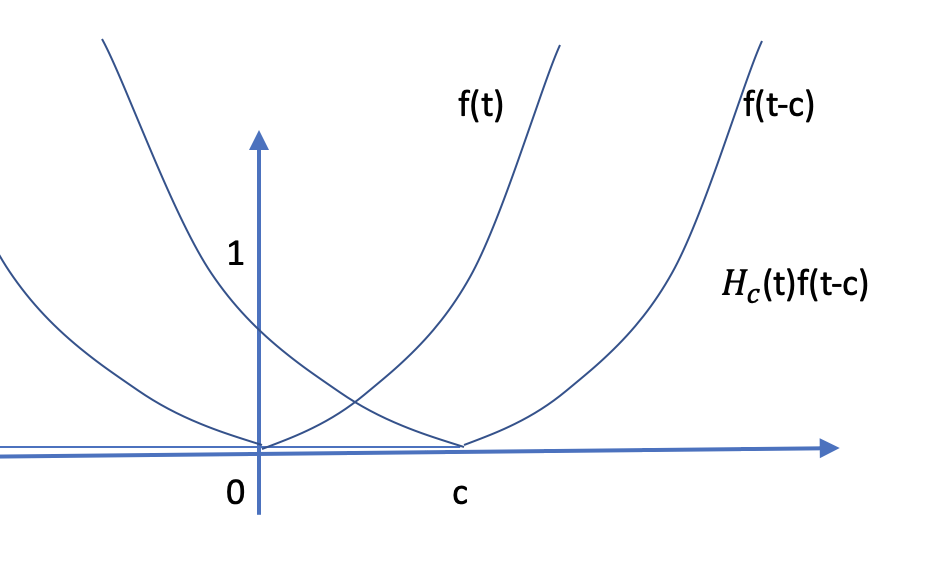
\includegraphics[width=8cm]{week9_3}
\end{figure}
\begin{proof}
\[\begin{aligned}
&\lapl{H_c(t)f(t-c)}(s)\\
=&\int_0^\infty e^{-st}H_c(t)f(t-c)\diff t\\
=&\int_c^\infty e^{-st}f(t-c)\diff t
\end{aligned}\]
$\bar{t}=t-c$
\[=\int_0^\infty e^{-s(\bar{t}+c)}f(\bar{t})\diff \bar{t}
\]
\[=\int_0^\infty e^{-s\bar{t}}f(\bar{t})\diff \bar{t} e^{-sc}
\]
\[=\lapl{f}(s)e^{-sc}
\]
\end{proof}
\begin{example}
\[y\pp-3y\p+2y=\begin{cases}\frac{1}{c},\quad 1<t<1+c\\0, \text{otherwise}\end{cases}
\]
\begin{figure}[H]
\centering
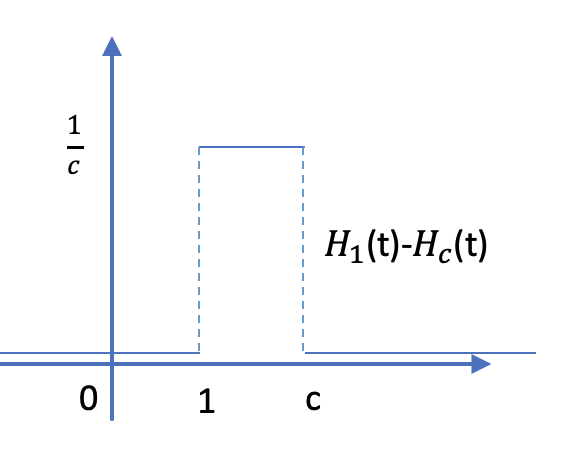
\includegraphics[width=6cm]{week9_4}
\end{figure}
\[Y=\lapl{y}\qquad y(0)=y\p(0)=0
\]
\[\begin{aligned}
&\lapl{y\pp-3y\p+2y}(s)\\
=&s^2Y(s)-3sY(s)+2Y(s)\\
=&Y(s)(s^2-3s+2)\dots(1)
\end{aligned}
\]
\[\begin{aligned}\lapl{\frac{1}{c}[H_1(t)-H_{1+c}(t)]}(s)&=\frac{1}{c}(\lapl{H_1(t)}(s)-\lapl{H_{1+c}(t)}(s))\\&=\frac{1}{c}(\frac{e^{-s}}{s}-\frac{e^{-(1+c)s}}{s})\dots(2)\end{aligned}
\]
(1)=(2), as we take laplace transformation on both side of the given equation in this example.
\[\begin{aligned}\therefore Y(s)&=\frac{\frac{1}{c}e^{-s}(1-e^{-cs})}{(s-1)(s-2)s}\\
&=\frac{1}{c}e^{-s}(1-e^{-cs})[\frac{1}{2s}-\frac{1}{s-1}+\frac{1}{2}\frac{1}{s-2}]\dots(3)\\
&=\frac{1}{c}e^{-s}(1-e^{-cs})\lapl{\frac{1}{2}-e^t+\frac{1}{2}e^{2t}}\dots(4)\\
&=\frac{1}{c}\lapl{H_1(t)[\frac{1}{2}-e^{t-1}+\frac{1}{2}e^{2(t-1)}]-H_{1+c}[\frac{1}{2}-e^{t-1-c}+\frac{1}{2}e^{2(t-1-c)}]}\dots(5)
\end{aligned}
\]
From (3) to (4), we do reverse laplace transformation, such as $\lapl{1}(s)=\int_0^\infty e^{-st}1\diff t=\dots=\frac{1}{s}$ and $\lapl{H_1(t)}(s)=e^{-s}\lapl{1}(s)$ (lemma above).\\
Procedure from (4) to (5) is due to lemma above.\\
Remember $Y(s)=\lapl{y}$
\[\begin{aligned}y(t)&=\frac{1}{c}\{H_1(t)[\frac{1}{2}-e^{t-1}+\frac{1}{2}e^{2(t-1)}]-H_{1+c}[\frac{1}{2}-e^{t-1-c}+\frac{1}{2}e^{2(t-1-c)}]\}\\
&=\frac{1}{c}\begin{cases}0,~t\leq1\\\frac{1}{2}-e^{t-1}+\frac{1}{2}e^{2(t-1)},~1<t<1+c\\-e^{t-1}+\frac{1}{2}e^{2(t-1)}+e^{t-1-c}-\frac{1}{2}e^{2(t-1-c)},~t\geq1+c\end{cases}
\end{aligned}
\]
As $c\rightarrow0$, $\frac{1}{2}e^{2(t-1)}\frac{1-e^{-2c}}{c}-e^{t-1}\frac{1-e^{-c}}{c}\rightarrow e^{2(t-1)}-e^{t-1}$ (by L'hospital's rule).

\end{example}

There is another way of doing this problem.
\begin{definition}[``Delta'' function: $\delta$] For any smooth function $\varphi$ with compact support on $\mathbb{R}$
\[\int_{-\infty}^\infty \delta(t)\varphi(t)\diff t=\varphi(0)
\]\end{definition}
\begin{example}[Example of delta function: ``Approximation to identity'']
A sequence of functions $\{\eta_\varepsilon\}$, $\eta(x)$ smooth supported inside $(-1,1)$, $\eta(-x)=\eta(x)\geq0$ and $\int_{-1}^1\eta(x)\diff x=1$\\
\[\eta(x)=\begin{cases}ce^{-\frac{1}{1-x^2}}~~|x|\leq1\\0~~|x|\geq1\end{cases}
\]
$c$ is chosen such that $\int_{-1}^1\eta=1$.
\[\eta_\varepsilon=\frac{1}{\varepsilon}\eta(\frac{x}{\varepsilon})
\]
 Want to show $\lim_{\varepsilon\rightarrow0}\eta_\varepsilon=\delta$, i.e. $\lim_{\varepsilon\rightarrow0}\int_{-\infty}^\infty\eta_\varepsilon(x)\varphi(x)\diff x=\varphi(0)$.
\end{example}
\begin{proof}
\[\int_{-\infty}^\infty\eta_\varepsilon(x)\diff x=1
\]
\[\begin{aligned}
|\int_{-\infty}^\infty\eta_\varepsilon(x)\varphi(x)\diff x-\varphi(0)|&=|\int_{-\infty}^\infty\eta_\varepsilon(x)\varphi(x)\diff x-\int_{-\infty}^\infty\eta_\varepsilon(x)\varphi(0)\diff x|\\
&\leq\int_{-\infty}^\infty|\eta_\varepsilon(x)[\varphi(x)-\varphi(0)]|\diff x=\int_{-\varepsilon}^\varepsilon\eta_\varepsilon(x)|\varphi(x)-\varphi(0)|\diff x\\
&\leq\int_{-\varepsilon}^\varepsilon\eta_{\varepsilon}(x)\diff x|\max_{|x|\leq\varepsilon}|\varphi(x)-\varphi(0)||\rightarrow0
\end{aligned}
\]




\end{proof}
\begin{remark}
Delta function isn't a function. As $\delta=\lim_{\varepsilon\rightarrow0}\eta_\varepsilon$, we can see delta function doesn't satisfy the definition of function at point 0. \\
In addition, the integral of delta function is equal to 1.

\end{remark}
\begin{example}
\[y\pp-3y\p+2y=\begin{cases}\frac{1}{c},~1<t<1+c\\0,~ \text{othrwise}\end{cases}
\]
\[y(0)=y\p(0)=0
\]
When $c\rightarrow0$, this question is the same as solve 
\[y\pp-3y\p+2y=\delta(t-1)
\]
\[Y(s)(s^2-3s+2)=\lapl{\delta(t-1)}(s)=\int_0^\infty e^{-st}\delta(t-1)\diff t
\]
\[\begin{aligned}
\therefore Y(s)&=\frac{e^{-s}}{(s-1)(s-2)}\\
&=e^{-s}(\frac{-1}{s-1}+\frac{1}{s-2})\\
&=\lapl{H_1(t)e^{t-1}+H_1(t)e^{2(t-1)}}(s)\\
&=\begin{cases}0,~t\leq1\\e^{2(t-1)}-e^{ct-1},~t\geq1\end{cases}
\end{aligned}
\]




\end{example}












\chapter{Week8}

\section{Monday}\index{Monday_lecture}
\subsection{Euler's Equation}
Recall previous knowledge,
\[t^2y\pp+\alpha ty\p+\beta y=0\qquad t>0
\]
$y=t^r$ $\Rightarrow\qquad$ $r(r-1)+\alpha r+\beta=0$ \\
$r^2+(\alpha-1)r+\beta=0$\\
$r_1,r_2=\frac{-(\alpha-1)\pm\sqrt{(\alpha-1)-4\beta}}{2}$
\begin{enumerate}
\item $(\alpha-1)^2-4\beta>0$  two real roots, $y=c_1t^{r_1}+c_2t^{r_2}$
\item $(\alpha-1)^2-4\beta=0$ $r_1=r_2=r$, $y=c_1t^r+c_2t^rlnt$
\item $(\alpha-1)^2-4\beta<0$ $r=\lambda\pm i\mu$, $y=t^\lambda[c_1\cos(\mu lnt)+c_2\sin(\mu lnt)]$
\end{enumerate}

Some motivations of Euler's Equation: Bessel's equation of order $\frac{1}{2}$\\
\[t^2y\pp+ty\p+(t^2-\frac{1}{4})y=0
\]
There doesn't exist a solution with the form of $y=\sum_{n=0}^\infty a_nt^n$. When $t=0$ it's a first order differential equation, the solution of this equation is only at one point $t=0$ which doesn't make much sense. We call this a singular point. We need to do something to factor out singularity.\\
\paragraph{Generalization}
\[L[y]\equiv t^2y\pp+t[p_0+p_1t+p_2t^2+\dots]y\p+[q_0+q_1t+q_2t^2+\dots]y=0
\]
Method of Frobenius,
\[y=\sum_{n=0}^\infty a_nt^{n+r}
\]
\begin{remark}
$r$ can be $\mathbb{R}$.\\
In order to avoid ambiguity, $a_0\neq 0$. Otherwise, it becomes $y=\sum_{n=1}^\infty a_nt^{n+r}$ which are the same as $y=\sum_{n=0}^{\infty}b_nt^{n+r\p}$. As $r$ and $r\p=r+1$ need to be determined, we have $y=\sum_{n=1}^\infty a_nt^{n+r}$ with the first term equals to zero, and $y=\sum_{n=0}^{\infty}b_nt^{n+r\p}$ to represent the same thing. Simply put, $a_0\neq 0$
\end{remark}
\[y\p=\sum_{n=0}^\infty(n+r)a_nt^{n+r-1}
\]
\[y\pp=\sum_{n=0}^{\infty}(n+r)(n+r-1)a_nt^{n+r-2}
\]
\[\begin{aligned}L[y]&=\sum_0^\infty(n+r)(n+r-1)a_nt^{n+r}+(\sum_{m=0}^\infty p_mt^m)(\sum_0^\infty (n+r)a_nt^{n+r})+\sum_{m=0}^\infty q_nt^m\sum_0^\infty a_nt^{n+r}\\
&=r(r-1)a_0+p_0ra_0+q_0a_0+[(1+r)ra_1+p_0(1+r)a_1+p_1ra_0+q_0a_1q_1a_0]t+\dots\\
&=[r(r-1)+p_0r+q_0]a_0+\underline{[\{(1+r)r+p_0(1+r)+q_0\}a_1+\{p_1r+q_1\}a_0]t}+\dots\\
&\quad+\underline{[(k+r)(k+r-1)a_k+\sum_{m=0}^kp_m(k-m+r)a_{k-m}+\sum_{n=0}^kq_ma_{k-m}]t^k}+\dots
\end{aligned}
\]
In order to have a solution $L[y]=0$,
Indicial equation
\[F(r)=r(r-1)+p_0r+q_0=0
\]
\[F(r+1)a_1=-[p_1r+q_1]a_0
\]
retrieved from first underline.\\Let's rewrite second underline a little bit.
\[=[(k+r)(k+r-1)a_k+\sum_0^{k-l}p_{k-l}(l+r)a_l+p_0a_k(k+r)+\sum_{n=1}^kq_{k-l}a_l+q_0a_k]t^k
\]
\[F(r+k)a_k=-[\sum_0^{k-1}\{p_{k-l}(l+1)+q_{k-l}\}a_l]
\]
It is clear that all $a_n$ can be solved recursively.\\
If there exists two real roots $r_1\geq r_2$, then 
\begin{itemize}
\item $r_1>r_2$ and $r_1-r_2$ is  not a positive integer. We will have two solutions.
\item $r_1>r_2$ and $r_1-r_2$ is a positive ineger then, you need to check textbook for more information as this will not be tested in the final.
\item $r_1=r_2$ check \textsection 2.8.3 for more information.
\end{itemize}
\begin{example}
\[t^2y\pp+ty\p+(-\frac{1}{4}+t^2)y=0
\]
$p_0=1$, $p_1=p_2=\dots=0$; $q=-\frac{1}{4}$, $q_1=0$, $q_2=1$, $q_3=0$\\Look at $L[y]\equiv t^2y\pp+t[p_0+p_1t+p_2t^2+\dots]y\p+[q_0+q_1t+q_2t^2+\dots]y=0$. You will know how we get all those stuffs.\\
$r(r-1)+r-\frac{1}{4}=0$, $r=\pm\frac{1}{2}$\\
First look at the first case $r=r_1=\frac{1}{2}$\\
$F(q+\frac{1}{2})a_1=0\Rightarrow a_1=0\dots(1)$ (We just pluge those stuffs in $F(r+1)a_1=-[p_1r+q_1]a_0$. \\
$F(k+r)a_k=k(k+1)a_k=-a_{k-2}\quad\Rightarrow ak=-\frac{1}{(k+1)ka_{k-2}}\dots(2)$  (As $F(k+r)=(r+k)^2-\frac{1}{4}=k(k+1)$)\\
With (1) and (2), we get $a_3=a_5=\dots=0$
\[a_2=-\frac{1}{3!}a_0
\]
\[a_4=-\frac{1}{5\cdot4}a_2=\frac{1}{5!}a_0
\]
\[a_{2n}=\frac{(-1)^n}{(2n+1)!}a_0
\]
\[y_1=a_0t^{\frac{1}{2}}(1-\frac{1}{3!}t^2+\frac{1}{5!}t^2-\dots)
\]
\[y_1=a_0t^{-\frac{1}{2}}\sin t
\]
$r_2=-\frac{1}{2}$
\[F(1+r_2)a_1=F(\frac{1}{2})a_1=0
\]
It's lucky both sides are equal to zero, else we cannot solve the second solution in this way.
\[F(k+r_2)=k(k-1)a_k=-q_2a_{k-2}=-a_{k-2}
\]
\[a_k=-\frac{1}{(k-1)k}a_{k-2}
\]
\[a_2=-\frac{1}{2}a_0
\]
\[a_4=-\frac{a_4}{4\cdot3}a_2=\frac{1}{4!}a_0
\]
\[a_6=-\frac{a_4}{6\cdot5}=-\frac{1}{6!}a_0
\]
\[y_2=t^{-\frac{1}{2}}a_0[1-\frac{1}{2!}t^2+\frac{1}{4!}t^4+\dots]=a_0t^{-\frac{1}{2}}\cos t
\]
Therefore, the general solutions is $y=\frac{1}{\sqrt{t}}(c_1\cos t+c_2\sin t)$
\end{example}



\section{Wednesday}\index{Wednesday_lecture}
\subsection{Application}
\paragraph{Mixture problem}There are two things that you need to bear in mind: \\\textcolor{red}{$\frac{\diff y}{\diff t}=$ input rate - output rate}, carry the units.

\begin{example}
A 120-gal tank initially contain 90kg salt dissoved in 90-gal of water. Brine containing 2kg/gal of salt flows into the tank at the water. Brine containing 2kg/gal of salt flows into the tank at the rate of 4gal/min, \& the well-stirned mixture flows out at the rate of 3 gal/min. How much salt does the tank contain when it is full?
\begin{figure}[H]
\centering
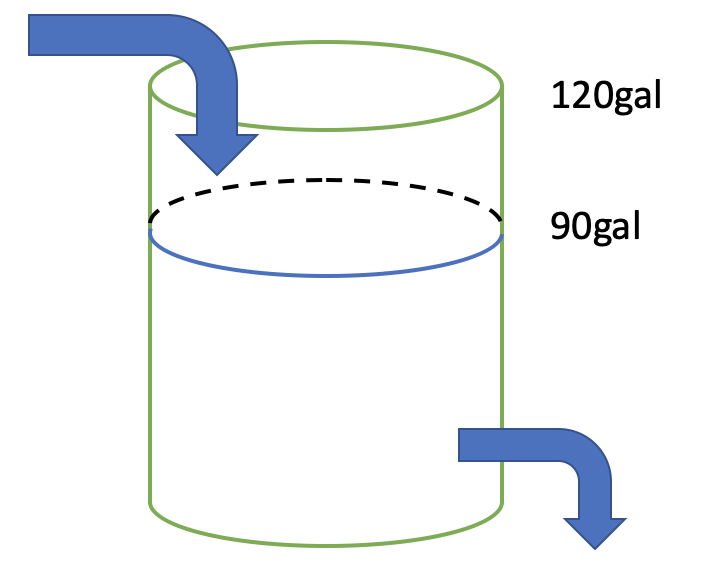
\includegraphics[width=5cm]{week2_wed_first}
\caption{First}
\end{figure}
Set $y(t)=$ the amount of salt at time $t$,\\ $V(t)=$the amount of brine at time $t$= 90 +$t$(gal)(t:minute)\\
\[\begin{aligned}y^\prime(t)&=2\text{kg/gal}\cdotp4\text{gal/min}-\frac{y(t)}{V(t)}\text{kg/gal}\cdotp3\text{gal/min}\\
&=8\text{kg/min}-3\frac{y(t)}{V(t)}\text{kg/min}
\end{aligned}
\]
\[y^\prime=8-3\frac{y}{90+t}
\]
\[y^\prime+\frac{3}{90+t}y=8
\]
By intergrating factor,
\[(e^{\int\frac{3}{90+t}\diff t}\cdotp y)^\prime=8e^{\int\frac{3}{90+t}\diff t}
\]
Try to simplify $e^{\int\frac{3}{90+t}\diff t}$;
\[\begin{aligned}\int\frac{3}{90+t}\diff t&=3ln|90+t|+\tilde{c}\\&=3ln(90+t)+\tilde{c}\end{aligned}
\]
Then,
\[e^{\int\frac{3}{90+t}\diff t}=(90+t)^3\cdotp c
\]
Integrate both sides,
\[(90+t)^3\cdotp c\cdotp y=8\int(90+t)^3\cdotp c\diff t
\]
\[(90+t)^3y=2\cdotp(90+t)^4+C
\]
\[y=2(90+t)+\frac{c}{(90+t)^3}
\]
\[y(0)=90=180+\frac{c}{90^3}\quad\Rightarrow\quad c=-90^4
\]
\[y=2(90+t)-\frac{90^4}{(90+t)^3}
\]
At $t=30$ the tank is full \& $y(30)=240-\frac{90^3}{120^3}\cdotp90$
\end{example}

\begin{example}[Persuit problem]
In a naval excercise, a distroyler $D$ is hunting a submarine $S$. Suppose $D$ at $(9,0)$ detects $S$ at $(0,0)$ \& at the same time $S$ detects $D$. Assuming that $S$ will dive immediately \& depart at full speed, $15$mile/hr in a straight course of unknown direction. What path should the destroyer $D$ follows to be certain of passing directly over the submarine $S$. If the speed of $D$ is $30$mile/hr at all time of the pursuit?
\begin{figure}[H]
\centering
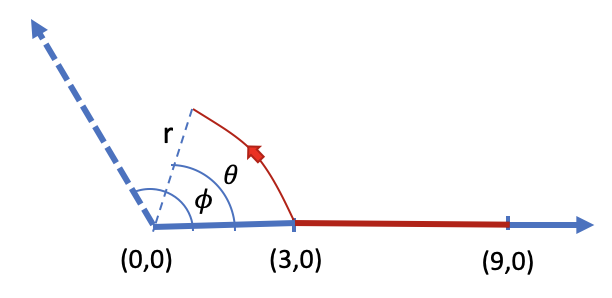
\includegraphics[width=8cm]{week2_wed_sec}
\caption{The path of destroyler in red.}
\end{figure}
Distance $D$ has travelled=$6+\int_0^\phi\sqrt{(r(\theta))^2+(r^\prime(\theta))^2}\diff\theta$.\\
Distance $S$ has travelled=$r(\phi)$.\\
For the speed of $D$ is twice than that of $S$, with the same period of time:
\[6+\int_0^\phi\sqrt{(r(\theta))^2+(r^\prime(\theta))^2}\diff\theta=2r(\phi)
\]
This isn't a form that can be dealt with. Differentiate both side,
\[\sqrt{(r(\phi))^2+(r^\prime(\phi))^2}=2r^\prime(\phi)
\]
\[(r(\phi))^2+(r^\prime(\phi))^2=4(r^\prime(\phi))^2
\]
\[r^\prime(\phi)=\pm\frac{1}{\sqrt{3}}r(\phi)
\]
W.L.O.G pick plus sign $\frac{r^\prime}{r}=\frac{1}{\sqrt{3}}$
\[lnr=\frac{1}{\sqrt{3}}\phi+\tilde{c}
\]
\[r=e^{\frac{\phi}{\sqrt{3}}}\cdotp c
\]
\[r(0)=3=c
\]
\[r(\phi)=3e^{\frac{\phi}{\sqrt{3}}}
\]
Given the direction $S$ take $\phi$, if $D$ want to be above it, they would reach each other at $(\phi,3e^{\frac{\phi}{\sqrt{3}}})$. This implies that if $D$ follows the path of 
$r(\theta)=3e^{\frac{\theta}{\sqrt{3}}}$, $D$ can catch $S$ whichever direction $S$ take.
\end{example}
\begin{remark}
There is a link about basic idea of how to compute the length of a curve:
\href{http://tutorial.math.lamar.edu/Classes/CalcII/ArcLength.aspx}{http://tutorial.math.lamar.edu/Classes/CalcII/ArcLength.aspx}. Check it if you are interested.
\end{remark}
\paragraph{Orthoganal trajectories} Given a family of curve $f(x,y,c)=0$. To find its orthoganal trajectories, the slope of the graph is needed. Differentiate $F$ by $x$;
\[F_x+F_yy_x=0
\]
Slope is $y_x=-\frac{F_x}{F_y}$. Then the slope of the graph that is orthoganal to the original one is \[y_x=\frac{F_y}{F_x}=\frac{\frac{\partial F}{\partial y}(x,y,c)}{\frac{\partial F}{\partial x}(x,y,c)}\]
\begin{example}
$y=cx^2$ $c$:parameter. To find another family of curves which is orthoganal to $y=cx^2$ whenever they intersect with each other.\\
$y=cx^2$, $\frac{\diff f}{\diff x}=2cx$ O.T. $\rightarrow \frac{\diff f}{\diff x}=\frac{-1}{2cx}=\frac{-1}{2\frac{y}{x^2}x}=-\frac{x}{2y}$ ( A separable equation)\\
$2y\diff y+x\diff x=0\quad\rightarrow\quad y^2+\frac{1}{2}x^2=c$
\end{example}



\chapter{Week8}

\section{Monday}\index{Monday_lecture}
\subsection{Euler's Equation}
Recall previous knowledge,
\[t^2y\pp+\alpha ty\p+\beta y=0\qquad t>0
\]
$y=t^r$ $\Rightarrow\qquad$ $r(r-1)+\alpha r+\beta=0$ \\
$r^2+(\alpha-1)r+\beta=0$\\
$r_1,r_2=\frac{-(\alpha-1)\pm\sqrt{(\alpha-1)-4\beta}}{2}$
\begin{enumerate}
\item $(\alpha-1)^2-4\beta>0$  two real roots, $y=c_1t^{r_1}+c_2t^{r_2}$
\item $(\alpha-1)^2-4\beta=0$ $r_1=r_2=r$, $y=c_1t^r+c_2t^rlnt$
\item $(\alpha-1)^2-4\beta<0$ $r=\lambda\pm i\mu$, $y=t^\lambda[c_1\cos(\mu lnt)+c_2\sin(\mu lnt)]$
\end{enumerate}

Some motivations of Euler's Equation: Bessel's equation of order $\frac{1}{2}$\\
\[t^2y\pp+ty\p+(t^2-\frac{1}{4})y=0
\]
There doesn't exist a solution with the form of $y=\sum_{n=0}^\infty a_nt^n$. When $t=0$ it's a first order differential equation, the solution of this equation is only at one point $t=0$ which doesn't make much sense. We call this a singular point. We need to do something to factor out singularity.\\
\paragraph{Generalization}
\[L[y]\equiv t^2y\pp+t[p_0+p_1t+p_2t^2+\dots]y\p+[q_0+q_1t+q_2t^2+\dots]y=0
\]
Method of Frobenius,
\[y=\sum_{n=0}^\infty a_nt^{n+r}
\]
\begin{remark}
$r$ can be $\mathbb{R}$.\\
In order to avoid ambiguity, $a_0\neq 0$. Otherwise, it becomes $y=\sum_{n=1}^\infty a_nt^{n+r}$ which are the same as $y=\sum_{n=0}^{\infty}b_nt^{n+r\p}$. As $r$ and $r\p=r+1$ need to be determined, we have $y=\sum_{n=1}^\infty a_nt^{n+r}$ with the first term equals to zero, and $y=\sum_{n=0}^{\infty}b_nt^{n+r\p}$ to represent the same thing. Simply put, $a_0\neq 0$
\end{remark}
\[y\p=\sum_{n=0}^\infty(n+r)a_nt^{n+r-1}
\]
\[y\pp=\sum_{n=0}^{\infty}(n+r)(n+r-1)a_nt^{n+r-2}
\]
\[\begin{aligned}L[y]&=\sum_0^\infty(n+r)(n+r-1)a_nt^{n+r}+(\sum_{m=0}^\infty p_mt^m)(\sum_0^\infty (n+r)a_nt^{n+r})+\sum_{m=0}^\infty q_nt^m\sum_0^\infty a_nt^{n+r}\\
&=r(r-1)a_0+p_0ra_0+q_0a_0+[(1+r)ra_1+p_0(1+r)a_1+p_1ra_0+q_0a_1q_1a_0]t+\dots\\
&=[r(r-1)+p_0r+q_0]a_0+\underline{[\{(1+r)r+p_0(1+r)+q_0\}a_1+\{p_1r+q_1\}a_0]t}+\dots\\
&\quad+\underline{[(k+r)(k+r-1)a_k+\sum_{m=0}^kp_m(k-m+r)a_{k-m}+\sum_{n=0}^kq_ma_{k-m}]t^k}+\dots
\end{aligned}
\]
In order to have a solution $L[y]=0$,
Indicial equation
\[F(r)=r(r-1)+p_0r+q_0=0
\]
\[F(r+1)a_1=-[p_1r+q_1]a_0
\]
retrieved from first underline.\\Let's rewrite second underline a little bit.
\[=[(k+r)(k+r-1)a_k+\sum_0^{k-l}p_{k-l}(l+r)a_l+p_0a_k(k+r)+\sum_{n=1}^kq_{k-l}a_l+q_0a_k]t^k
\]
\[F(r+k)a_k=-[\sum_0^{k-1}\{p_{k-l}(l+1)+q_{k-l}\}a_l]
\]
It is clear that all $a_n$ can be solved recursively.\\
If there exists two real roots $r_1\geq r_2$, then 
\begin{itemize}
\item $r_1>r_2$ and $r_1-r_2$ is  not a positive integer. We will have two solutions.
\item $r_1>r_2$ and $r_1-r_2$ is a positive ineger then, you need to check textbook for more information as this will not be tested in the final.
\item $r_1=r_2$ check \textsection 2.8.3 for more information.
\end{itemize}
\begin{example}
\[t^2y\pp+ty\p+(-\frac{1}{4}+t^2)y=0
\]
$p_0=1$, $p_1=p_2=\dots=0$; $q=-\frac{1}{4}$, $q_1=0$, $q_2=1$, $q_3=0$\\Look at $L[y]\equiv t^2y\pp+t[p_0+p_1t+p_2t^2+\dots]y\p+[q_0+q_1t+q_2t^2+\dots]y=0$. You will know how we get all those stuffs.\\
$r(r-1)+r-\frac{1}{4}=0$, $r=\pm\frac{1}{2}$\\
First look at the first case $r=r_1=\frac{1}{2}$\\
$F(q+\frac{1}{2})a_1=0\Rightarrow a_1=0\dots(1)$ (We just pluge those stuffs in $F(r+1)a_1=-[p_1r+q_1]a_0$. \\
$F(k+r)a_k=k(k+1)a_k=-a_{k-2}\quad\Rightarrow ak=-\frac{1}{(k+1)ka_{k-2}}\dots(2)$  (As $F(k+r)=(r+k)^2-\frac{1}{4}=k(k+1)$)\\
With (1) and (2), we get $a_3=a_5=\dots=0$
\[a_2=-\frac{1}{3!}a_0
\]
\[a_4=-\frac{1}{5\cdot4}a_2=\frac{1}{5!}a_0
\]
\[a_{2n}=\frac{(-1)^n}{(2n+1)!}a_0
\]
\[y_1=a_0t^{\frac{1}{2}}(1-\frac{1}{3!}t^2+\frac{1}{5!}t^2-\dots)
\]
\[y_1=a_0t^{-\frac{1}{2}}\sin t
\]
$r_2=-\frac{1}{2}$
\[F(1+r_2)a_1=F(\frac{1}{2})a_1=0
\]
It's lucky both sides are equal to zero, else we cannot solve the second solution in this way.
\[F(k+r_2)=k(k-1)a_k=-q_2a_{k-2}=-a_{k-2}
\]
\[a_k=-\frac{1}{(k-1)k}a_{k-2}
\]
\[a_2=-\frac{1}{2}a_0
\]
\[a_4=-\frac{a_4}{4\cdot3}a_2=\frac{1}{4!}a_0
\]
\[a_6=-\frac{a_4}{6\cdot5}=-\frac{1}{6!}a_0
\]
\[y_2=t^{-\frac{1}{2}}a_0[1-\frac{1}{2!}t^2+\frac{1}{4!}t^4+\dots]=a_0t^{-\frac{1}{2}}\cos t
\]
Therefore, the general solutions is $y=\frac{1}{\sqrt{t}}(c_1\cos t+c_2\sin t)$
\end{example}



\section{Wednesday}\index{Wednesday_lecture}
\subsection{Application}
\paragraph{Mixture problem}There are two things that you need to bear in mind: \\\textcolor{red}{$\frac{\diff y}{\diff t}=$ input rate - output rate}, carry the units.

\begin{example}
A 120-gal tank initially contain 90kg salt dissoved in 90-gal of water. Brine containing 2kg/gal of salt flows into the tank at the water. Brine containing 2kg/gal of salt flows into the tank at the rate of 4gal/min, \& the well-stirned mixture flows out at the rate of 3 gal/min. How much salt does the tank contain when it is full?
\begin{figure}[H]
\centering
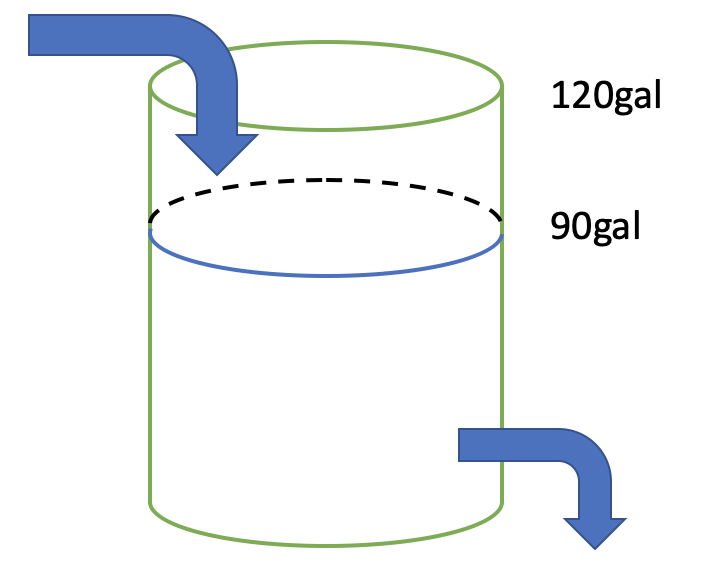
\includegraphics[width=5cm]{week2_wed_first}
\caption{First}
\end{figure}
Set $y(t)=$ the amount of salt at time $t$,\\ $V(t)=$the amount of brine at time $t$= 90 +$t$(gal)(t:minute)\\
\[\begin{aligned}y^\prime(t)&=2\text{kg/gal}\cdotp4\text{gal/min}-\frac{y(t)}{V(t)}\text{kg/gal}\cdotp3\text{gal/min}\\
&=8\text{kg/min}-3\frac{y(t)}{V(t)}\text{kg/min}
\end{aligned}
\]
\[y^\prime=8-3\frac{y}{90+t}
\]
\[y^\prime+\frac{3}{90+t}y=8
\]
By intergrating factor,
\[(e^{\int\frac{3}{90+t}\diff t}\cdotp y)^\prime=8e^{\int\frac{3}{90+t}\diff t}
\]
Try to simplify $e^{\int\frac{3}{90+t}\diff t}$;
\[\begin{aligned}\int\frac{3}{90+t}\diff t&=3ln|90+t|+\tilde{c}\\&=3ln(90+t)+\tilde{c}\end{aligned}
\]
Then,
\[e^{\int\frac{3}{90+t}\diff t}=(90+t)^3\cdotp c
\]
Integrate both sides,
\[(90+t)^3\cdotp c\cdotp y=8\int(90+t)^3\cdotp c\diff t
\]
\[(90+t)^3y=2\cdotp(90+t)^4+C
\]
\[y=2(90+t)+\frac{c}{(90+t)^3}
\]
\[y(0)=90=180+\frac{c}{90^3}\quad\Rightarrow\quad c=-90^4
\]
\[y=2(90+t)-\frac{90^4}{(90+t)^3}
\]
At $t=30$ the tank is full \& $y(30)=240-\frac{90^3}{120^3}\cdotp90$
\end{example}

\begin{example}[Persuit problem]
In a naval excercise, a distroyler $D$ is hunting a submarine $S$. Suppose $D$ at $(9,0)$ detects $S$ at $(0,0)$ \& at the same time $S$ detects $D$. Assuming that $S$ will dive immediately \& depart at full speed, $15$mile/hr in a straight course of unknown direction. What path should the destroyer $D$ follows to be certain of passing directly over the submarine $S$. If the speed of $D$ is $30$mile/hr at all time of the pursuit?
\begin{figure}[H]
\centering
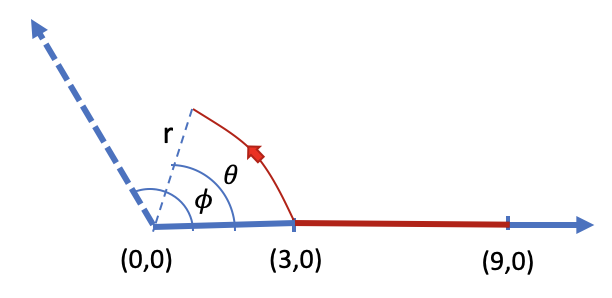
\includegraphics[width=8cm]{week2_wed_sec}
\caption{The path of destroyler in red.}
\end{figure}
Distance $D$ has travelled=$6+\int_0^\phi\sqrt{(r(\theta))^2+(r^\prime(\theta))^2}\diff\theta$.\\
Distance $S$ has travelled=$r(\phi)$.\\
For the speed of $D$ is twice than that of $S$, with the same period of time:
\[6+\int_0^\phi\sqrt{(r(\theta))^2+(r^\prime(\theta))^2}\diff\theta=2r(\phi)
\]
This isn't a form that can be dealt with. Differentiate both side,
\[\sqrt{(r(\phi))^2+(r^\prime(\phi))^2}=2r^\prime(\phi)
\]
\[(r(\phi))^2+(r^\prime(\phi))^2=4(r^\prime(\phi))^2
\]
\[r^\prime(\phi)=\pm\frac{1}{\sqrt{3}}r(\phi)
\]
W.L.O.G pick plus sign $\frac{r^\prime}{r}=\frac{1}{\sqrt{3}}$
\[lnr=\frac{1}{\sqrt{3}}\phi+\tilde{c}
\]
\[r=e^{\frac{\phi}{\sqrt{3}}}\cdotp c
\]
\[r(0)=3=c
\]
\[r(\phi)=3e^{\frac{\phi}{\sqrt{3}}}
\]
Given the direction $S$ take $\phi$, if $D$ want to be above it, they would reach each other at $(\phi,3e^{\frac{\phi}{\sqrt{3}}})$. This implies that if $D$ follows the path of 
$r(\theta)=3e^{\frac{\theta}{\sqrt{3}}}$, $D$ can catch $S$ whichever direction $S$ take.
\end{example}
\begin{remark}
There is a link about basic idea of how to compute the length of a curve:
\href{http://tutorial.math.lamar.edu/Classes/CalcII/ArcLength.aspx}{http://tutorial.math.lamar.edu/Classes/CalcII/ArcLength.aspx}. Check it if you are interested.
\end{remark}
\paragraph{Orthoganal trajectories} Given a family of curve $f(x,y,c)=0$. To find its orthoganal trajectories, the slope of the graph is needed. Differentiate $F$ by $x$;
\[F_x+F_yy_x=0
\]
Slope is $y_x=-\frac{F_x}{F_y}$. Then the slope of the graph that is orthoganal to the original one is \[y_x=\frac{F_y}{F_x}=\frac{\frac{\partial F}{\partial y}(x,y,c)}{\frac{\partial F}{\partial x}(x,y,c)}\]
\begin{example}
$y=cx^2$ $c$:parameter. To find another family of curves which is orthoganal to $y=cx^2$ whenever they intersect with each other.\\
$y=cx^2$, $\frac{\diff f}{\diff x}=2cx$ O.T. $\rightarrow \frac{\diff f}{\diff x}=\frac{-1}{2cx}=\frac{-1}{2\frac{y}{x^2}x}=-\frac{x}{2y}$ ( A separable equation)\\
$2y\diff y+x\diff x=0\quad\rightarrow\quad y^2+\frac{1}{2}x^2=c$
\end{example}



\chapter{Week8}

\section{Monday}\index{Monday_lecture}
\subsection{Euler's Equation}
Recall previous knowledge,
\[t^2y\pp+\alpha ty\p+\beta y=0\qquad t>0
\]
$y=t^r$ $\Rightarrow\qquad$ $r(r-1)+\alpha r+\beta=0$ \\
$r^2+(\alpha-1)r+\beta=0$\\
$r_1,r_2=\frac{-(\alpha-1)\pm\sqrt{(\alpha-1)-4\beta}}{2}$
\begin{enumerate}
\item $(\alpha-1)^2-4\beta>0$  two real roots, $y=c_1t^{r_1}+c_2t^{r_2}$
\item $(\alpha-1)^2-4\beta=0$ $r_1=r_2=r$, $y=c_1t^r+c_2t^rlnt$
\item $(\alpha-1)^2-4\beta<0$ $r=\lambda\pm i\mu$, $y=t^\lambda[c_1\cos(\mu lnt)+c_2\sin(\mu lnt)]$
\end{enumerate}

Some motivations of Euler's Equation: Bessel's equation of order $\frac{1}{2}$\\
\[t^2y\pp+ty\p+(t^2-\frac{1}{4})y=0
\]
There doesn't exist a solution with the form of $y=\sum_{n=0}^\infty a_nt^n$. When $t=0$ it's a first order differential equation, the solution of this equation is only at one point $t=0$ which doesn't make much sense. We call this a singular point. We need to do something to factor out singularity.\\
\paragraph{Generalization}
\[L[y]\equiv t^2y\pp+t[p_0+p_1t+p_2t^2+\dots]y\p+[q_0+q_1t+q_2t^2+\dots]y=0
\]
Method of Frobenius,
\[y=\sum_{n=0}^\infty a_nt^{n+r}
\]
\begin{remark}
$r$ can be $\mathbb{R}$.\\
In order to avoid ambiguity, $a_0\neq 0$. Otherwise, it becomes $y=\sum_{n=1}^\infty a_nt^{n+r}$ which are the same as $y=\sum_{n=0}^{\infty}b_nt^{n+r\p}$. As $r$ and $r\p=r+1$ need to be determined, we have $y=\sum_{n=1}^\infty a_nt^{n+r}$ with the first term equals to zero, and $y=\sum_{n=0}^{\infty}b_nt^{n+r\p}$ to represent the same thing. Simply put, $a_0\neq 0$
\end{remark}
\[y\p=\sum_{n=0}^\infty(n+r)a_nt^{n+r-1}
\]
\[y\pp=\sum_{n=0}^{\infty}(n+r)(n+r-1)a_nt^{n+r-2}
\]
\[\begin{aligned}L[y]&=\sum_0^\infty(n+r)(n+r-1)a_nt^{n+r}+(\sum_{m=0}^\infty p_mt^m)(\sum_0^\infty (n+r)a_nt^{n+r})+\sum_{m=0}^\infty q_nt^m\sum_0^\infty a_nt^{n+r}\\
&=r(r-1)a_0+p_0ra_0+q_0a_0+[(1+r)ra_1+p_0(1+r)a_1+p_1ra_0+q_0a_1q_1a_0]t+\dots\\
&=[r(r-1)+p_0r+q_0]a_0+\underline{[\{(1+r)r+p_0(1+r)+q_0\}a_1+\{p_1r+q_1\}a_0]t}+\dots\\
&\quad+\underline{[(k+r)(k+r-1)a_k+\sum_{m=0}^kp_m(k-m+r)a_{k-m}+\sum_{n=0}^kq_ma_{k-m}]t^k}+\dots
\end{aligned}
\]
In order to have a solution $L[y]=0$,
Indicial equation
\[F(r)=r(r-1)+p_0r+q_0=0
\]
\[F(r+1)a_1=-[p_1r+q_1]a_0
\]
retrieved from first underline.\\Let's rewrite second underline a little bit.
\[=[(k+r)(k+r-1)a_k+\sum_0^{k-l}p_{k-l}(l+r)a_l+p_0a_k(k+r)+\sum_{n=1}^kq_{k-l}a_l+q_0a_k]t^k
\]
\[F(r+k)a_k=-[\sum_0^{k-1}\{p_{k-l}(l+1)+q_{k-l}\}a_l]
\]
It is clear that all $a_n$ can be solved recursively.\\
If there exists two real roots $r_1\geq r_2$, then 
\begin{itemize}
\item $r_1>r_2$ and $r_1-r_2$ is  not a positive integer. We will have two solutions.
\item $r_1>r_2$ and $r_1-r_2$ is a positive ineger then, you need to check textbook for more information as this will not be tested in the final.
\item $r_1=r_2$ check \textsection 2.8.3 for more information.
\end{itemize}
\begin{example}
\[t^2y\pp+ty\p+(-\frac{1}{4}+t^2)y=0
\]
$p_0=1$, $p_1=p_2=\dots=0$; $q=-\frac{1}{4}$, $q_1=0$, $q_2=1$, $q_3=0$\\Look at $L[y]\equiv t^2y\pp+t[p_0+p_1t+p_2t^2+\dots]y\p+[q_0+q_1t+q_2t^2+\dots]y=0$. You will know how we get all those stuffs.\\
$r(r-1)+r-\frac{1}{4}=0$, $r=\pm\frac{1}{2}$\\
First look at the first case $r=r_1=\frac{1}{2}$\\
$F(q+\frac{1}{2})a_1=0\Rightarrow a_1=0\dots(1)$ (We just pluge those stuffs in $F(r+1)a_1=-[p_1r+q_1]a_0$. \\
$F(k+r)a_k=k(k+1)a_k=-a_{k-2}\quad\Rightarrow ak=-\frac{1}{(k+1)ka_{k-2}}\dots(2)$  (As $F(k+r)=(r+k)^2-\frac{1}{4}=k(k+1)$)\\
With (1) and (2), we get $a_3=a_5=\dots=0$
\[a_2=-\frac{1}{3!}a_0
\]
\[a_4=-\frac{1}{5\cdot4}a_2=\frac{1}{5!}a_0
\]
\[a_{2n}=\frac{(-1)^n}{(2n+1)!}a_0
\]
\[y_1=a_0t^{\frac{1}{2}}(1-\frac{1}{3!}t^2+\frac{1}{5!}t^2-\dots)
\]
\[y_1=a_0t^{-\frac{1}{2}}\sin t
\]
$r_2=-\frac{1}{2}$
\[F(1+r_2)a_1=F(\frac{1}{2})a_1=0
\]
It's lucky both sides are equal to zero, else we cannot solve the second solution in this way.
\[F(k+r_2)=k(k-1)a_k=-q_2a_{k-2}=-a_{k-2}
\]
\[a_k=-\frac{1}{(k-1)k}a_{k-2}
\]
\[a_2=-\frac{1}{2}a_0
\]
\[a_4=-\frac{a_4}{4\cdot3}a_2=\frac{1}{4!}a_0
\]
\[a_6=-\frac{a_4}{6\cdot5}=-\frac{1}{6!}a_0
\]
\[y_2=t^{-\frac{1}{2}}a_0[1-\frac{1}{2!}t^2+\frac{1}{4!}t^4+\dots]=a_0t^{-\frac{1}{2}}\cos t
\]
Therefore, the general solutions is $y=\frac{1}{\sqrt{t}}(c_1\cos t+c_2\sin t)$
\end{example}



\section{Wednesday}\index{Wednesday_lecture}
\subsection{Laplace Transformation}
\[\lapl{f}(s)=\int_0^\infty e^{-st}f(t)\diff t
\]
\[|f(t)\leq Me^{ct}|\qquad\text{for t large, } s>c
\]
Heariside function $H(t)$
\begin{figure}[H]
\centering
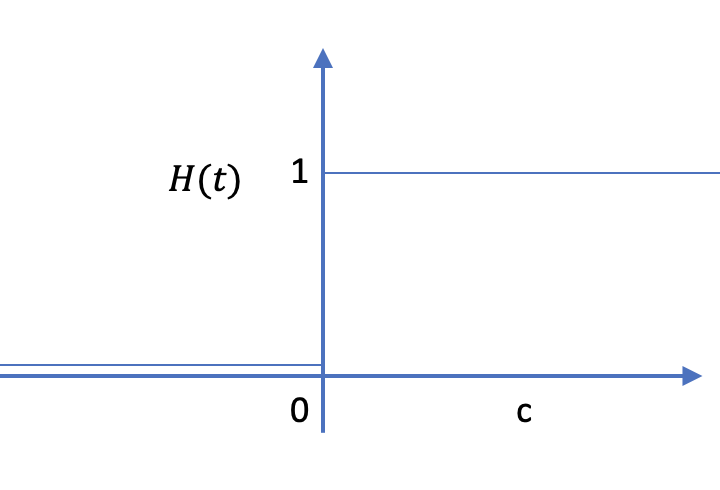
\includegraphics[width=6cm]{week9_1}
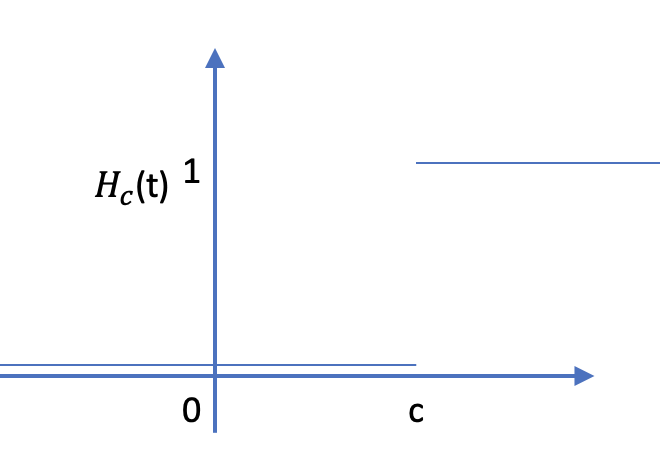
\includegraphics[width=6cm]{week9_2}
\end{figure}

\paragraph{lemma}
\[\lapl{H_c(t)f(t-c)}(s)=e^{-cs}F(s)\]
($F(s)=\lapl{f}(s)$)
\begin{figure}[H]
\centering
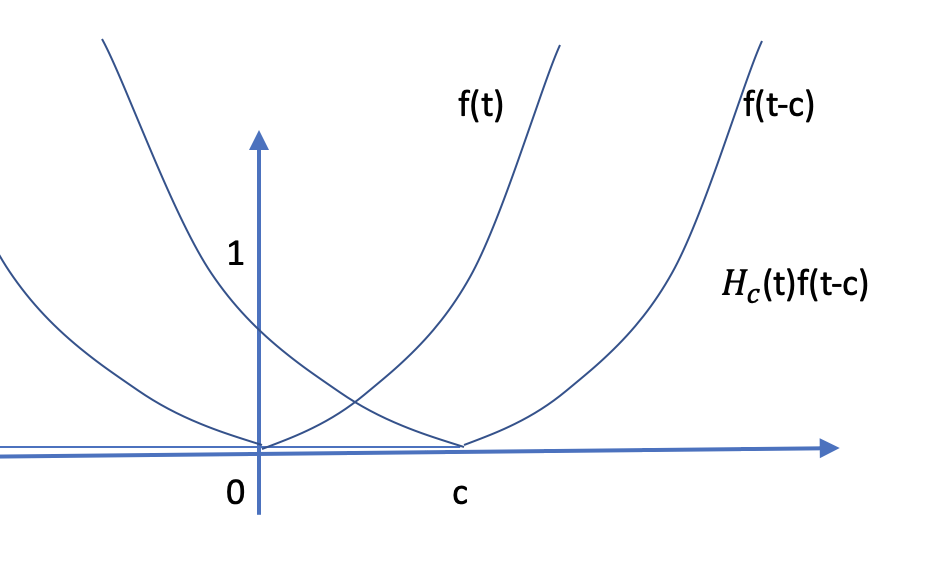
\includegraphics[width=8cm]{week9_3}
\end{figure}
\begin{proof}
\[\begin{aligned}
&\lapl{H_c(t)f(t-c)}(s)\\
=&\int_0^\infty e^{-st}H_c(t)f(t-c)\diff t\\
=&\int_c^\infty e^{-st}f(t-c)\diff t
\end{aligned}\]
$\bar{t}=t-c$
\[=\int_0^\infty e^{-s(\bar{t}+c)}f(\bar{t})\diff \bar{t}
\]
\[=\int_0^\infty e^{-s\bar{t}}f(\bar{t})\diff \bar{t} e^{-sc}
\]
\[=\lapl{f}(s)e^{-sc}
\]
\end{proof}
\begin{example}
\[y\pp-3y\p+2y=\begin{cases}\frac{1}{c},\quad 1<t<1+c\\0, \text{otherwise}\end{cases}
\]
\begin{figure}[H]
\centering
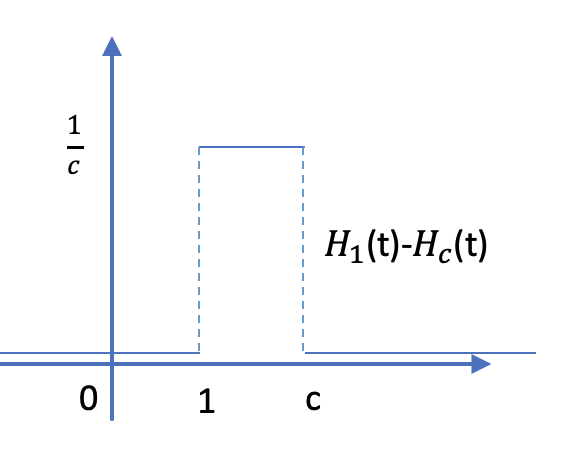
\includegraphics[width=6cm]{week9_4}
\end{figure}
\[Y=\lapl{y}\qquad y(0)=y\p(0)=0
\]
\[\begin{aligned}
&\lapl{y\pp-3y\p+2y}(s)\\
=&s^2Y(s)-3sY(s)+2Y(s)\\
=&Y(s)(s^2-3s+2)\dots(1)
\end{aligned}
\]
\[\begin{aligned}\lapl{\frac{1}{c}[H_1(t)-H_{1+c}(t)]}(s)&=\frac{1}{c}(\lapl{H_1(t)}(s)-\lapl{H_{1+c}(t)}(s))\\&=\frac{1}{c}(\frac{e^{-s}}{s}-\frac{e^{-(1+c)s}}{s})\dots(2)\end{aligned}
\]
(1)=(2), as we take laplace transformation on both side of the given equation in this example.
\[\begin{aligned}\therefore Y(s)&=\frac{\frac{1}{c}e^{-s}(1-e^{-cs})}{(s-1)(s-2)s}\\
&=\frac{1}{c}e^{-s}(1-e^{-cs})[\frac{1}{2s}-\frac{1}{s-1}+\frac{1}{2}\frac{1}{s-2}]\dots(3)\\
&=\frac{1}{c}e^{-s}(1-e^{-cs})\lapl{\frac{1}{2}-e^t+\frac{1}{2}e^{2t}}\dots(4)\\
&=\frac{1}{c}\lapl{H_1(t)[\frac{1}{2}-e^{t-1}+\frac{1}{2}e^{2(t-1)}]-H_{1+c}[\frac{1}{2}-e^{t-1-c}+\frac{1}{2}e^{2(t-1-c)}]}\dots(5)
\end{aligned}
\]
From (3) to (4), we do reverse laplace transformation, such as $\lapl{1}(s)=\int_0^\infty e^{-st}1\diff t=\dots=\frac{1}{s}$ and $\lapl{H_1(t)}(s)=e^{-s}\lapl{1}(s)$ (lemma above).\\
Procedure from (4) to (5) is due to lemma above.\\
Remember $Y(s)=\lapl{y}$
\[\begin{aligned}y(t)&=\frac{1}{c}\{H_1(t)[\frac{1}{2}-e^{t-1}+\frac{1}{2}e^{2(t-1)}]-H_{1+c}[\frac{1}{2}-e^{t-1-c}+\frac{1}{2}e^{2(t-1-c)}]\}\\
&=\frac{1}{c}\begin{cases}0,~t\leq1\\\frac{1}{2}-e^{t-1}+\frac{1}{2}e^{2(t-1)},~1<t<1+c\\-e^{t-1}+\frac{1}{2}e^{2(t-1)}+e^{t-1-c}-\frac{1}{2}e^{2(t-1-c)},~t\geq1+c\end{cases}
\end{aligned}
\]
As $c\rightarrow0$, $\frac{1}{2}e^{2(t-1)}\frac{1-e^{-2c}}{c}-e^{t-1}\frac{1-e^{-c}}{c}\rightarrow e^{2(t-1)}-e^{t-1}$ (by L'hospital's rule).

\end{example}

There is another way of doing this problem.
\begin{definition}[``Delta'' function: $\delta$] For any smooth function $\varphi$ with compact support on $\mathbb{R}$
\[\int_{-\infty}^\infty \delta(t)\varphi(t)\diff t=\varphi(0)
\]\end{definition}
\begin{example}[Example of delta function: ``Approximation to identity'']
A sequence of functions $\{\eta_\varepsilon\}$, $\eta(x)$ smooth supported inside $(-1,1)$, $\eta(-x)=\eta(x)\geq0$ and $\int_{-1}^1\eta(x)\diff x=1$\\
\[\eta(x)=\begin{cases}ce^{-\frac{1}{1-x^2}}~~|x|\leq1\\0~~|x|\geq1\end{cases}
\]
$c$ is chosen such that $\int_{-1}^1\eta=1$.
\[\eta_\varepsilon=\frac{1}{\varepsilon}\eta(\frac{x}{\varepsilon})
\]
 Want to show $\lim_{\varepsilon\rightarrow0}\eta_\varepsilon=\delta$, i.e. $\lim_{\varepsilon\rightarrow0}\int_{-\infty}^\infty\eta_\varepsilon(x)\varphi(x)\diff x=\varphi(0)$.
\end{example}
\begin{proof}
\[\int_{-\infty}^\infty\eta_\varepsilon(x)\diff x=1
\]
\[\begin{aligned}
|\int_{-\infty}^\infty\eta_\varepsilon(x)\varphi(x)\diff x-\varphi(0)|&=|\int_{-\infty}^\infty\eta_\varepsilon(x)\varphi(x)\diff x-\int_{-\infty}^\infty\eta_\varepsilon(x)\varphi(0)\diff x|\\
&\leq\int_{-\infty}^\infty|\eta_\varepsilon(x)[\varphi(x)-\varphi(0)]|\diff x=\int_{-\varepsilon}^\varepsilon\eta_\varepsilon(x)|\varphi(x)-\varphi(0)|\diff x\\
&\leq\int_{-\varepsilon}^\varepsilon\eta_{\varepsilon}(x)\diff x|\max_{|x|\leq\varepsilon}|\varphi(x)-\varphi(0)||\rightarrow0
\end{aligned}
\]




\end{proof}
\begin{remark}
Delta function isn't a function. As $\delta=\lim_{\varepsilon\rightarrow0}\eta_\varepsilon$, we can see delta function doesn't satisfy the definition of function at point 0. \\
In addition, the integral of delta function is equal to 1.

\end{remark}
\begin{example}
\[y\pp-3y\p+2y=\begin{cases}\frac{1}{c},~1<t<1+c\\0,~ \text{othrwise}\end{cases}
\]
\[y(0)=y\p(0)=0
\]
When $c\rightarrow0$, this question is the same as solve 
\[y\pp-3y\p+2y=\delta(t-1)
\]
\[Y(s)(s^2-3s+2)=\lapl{\delta(t-1)}(s)=\int_0^\infty e^{-st}\delta(t-1)\diff t
\]
\[\begin{aligned}
\therefore Y(s)&=\frac{e^{-s}}{(s-1)(s-2)}\\
&=e^{-s}(\frac{-1}{s-1}+\frac{1}{s-2})\\
&=\lapl{H_1(t)e^{t-1}+H_1(t)e^{2(t-1)}}(s)\\
&=\begin{cases}0,~t\leq1\\e^{2(t-1)}-e^{ct-1},~t\geq1\end{cases}
\end{aligned}
\]




\end{example}












\include{4.27/4.27}
\chapter{Week8}

\section{Monday}\index{Monday_lecture}
\subsection{Euler's Equation}
Recall previous knowledge,
\[t^2y\pp+\alpha ty\p+\beta y=0\qquad t>0
\]
$y=t^r$ $\Rightarrow\qquad$ $r(r-1)+\alpha r+\beta=0$ \\
$r^2+(\alpha-1)r+\beta=0$\\
$r_1,r_2=\frac{-(\alpha-1)\pm\sqrt{(\alpha-1)-4\beta}}{2}$
\begin{enumerate}
\item $(\alpha-1)^2-4\beta>0$  two real roots, $y=c_1t^{r_1}+c_2t^{r_2}$
\item $(\alpha-1)^2-4\beta=0$ $r_1=r_2=r$, $y=c_1t^r+c_2t^rlnt$
\item $(\alpha-1)^2-4\beta<0$ $r=\lambda\pm i\mu$, $y=t^\lambda[c_1\cos(\mu lnt)+c_2\sin(\mu lnt)]$
\end{enumerate}

Some motivations of Euler's Equation: Bessel's equation of order $\frac{1}{2}$\\
\[t^2y\pp+ty\p+(t^2-\frac{1}{4})y=0
\]
There doesn't exist a solution with the form of $y=\sum_{n=0}^\infty a_nt^n$. When $t=0$ it's a first order differential equation, the solution of this equation is only at one point $t=0$ which doesn't make much sense. We call this a singular point. We need to do something to factor out singularity.\\
\paragraph{Generalization}
\[L[y]\equiv t^2y\pp+t[p_0+p_1t+p_2t^2+\dots]y\p+[q_0+q_1t+q_2t^2+\dots]y=0
\]
Method of Frobenius,
\[y=\sum_{n=0}^\infty a_nt^{n+r}
\]
\begin{remark}
$r$ can be $\mathbb{R}$.\\
In order to avoid ambiguity, $a_0\neq 0$. Otherwise, it becomes $y=\sum_{n=1}^\infty a_nt^{n+r}$ which are the same as $y=\sum_{n=0}^{\infty}b_nt^{n+r\p}$. As $r$ and $r\p=r+1$ need to be determined, we have $y=\sum_{n=1}^\infty a_nt^{n+r}$ with the first term equals to zero, and $y=\sum_{n=0}^{\infty}b_nt^{n+r\p}$ to represent the same thing. Simply put, $a_0\neq 0$
\end{remark}
\[y\p=\sum_{n=0}^\infty(n+r)a_nt^{n+r-1}
\]
\[y\pp=\sum_{n=0}^{\infty}(n+r)(n+r-1)a_nt^{n+r-2}
\]
\[\begin{aligned}L[y]&=\sum_0^\infty(n+r)(n+r-1)a_nt^{n+r}+(\sum_{m=0}^\infty p_mt^m)(\sum_0^\infty (n+r)a_nt^{n+r})+\sum_{m=0}^\infty q_nt^m\sum_0^\infty a_nt^{n+r}\\
&=r(r-1)a_0+p_0ra_0+q_0a_0+[(1+r)ra_1+p_0(1+r)a_1+p_1ra_0+q_0a_1q_1a_0]t+\dots\\
&=[r(r-1)+p_0r+q_0]a_0+\underline{[\{(1+r)r+p_0(1+r)+q_0\}a_1+\{p_1r+q_1\}a_0]t}+\dots\\
&\quad+\underline{[(k+r)(k+r-1)a_k+\sum_{m=0}^kp_m(k-m+r)a_{k-m}+\sum_{n=0}^kq_ma_{k-m}]t^k}+\dots
\end{aligned}
\]
In order to have a solution $L[y]=0$,
Indicial equation
\[F(r)=r(r-1)+p_0r+q_0=0
\]
\[F(r+1)a_1=-[p_1r+q_1]a_0
\]
retrieved from first underline.\\Let's rewrite second underline a little bit.
\[=[(k+r)(k+r-1)a_k+\sum_0^{k-l}p_{k-l}(l+r)a_l+p_0a_k(k+r)+\sum_{n=1}^kq_{k-l}a_l+q_0a_k]t^k
\]
\[F(r+k)a_k=-[\sum_0^{k-1}\{p_{k-l}(l+1)+q_{k-l}\}a_l]
\]
It is clear that all $a_n$ can be solved recursively.\\
If there exists two real roots $r_1\geq r_2$, then 
\begin{itemize}
\item $r_1>r_2$ and $r_1-r_2$ is  not a positive integer. We will have two solutions.
\item $r_1>r_2$ and $r_1-r_2$ is a positive ineger then, you need to check textbook for more information as this will not be tested in the final.
\item $r_1=r_2$ check \textsection 2.8.3 for more information.
\end{itemize}
\begin{example}
\[t^2y\pp+ty\p+(-\frac{1}{4}+t^2)y=0
\]
$p_0=1$, $p_1=p_2=\dots=0$; $q=-\frac{1}{4}$, $q_1=0$, $q_2=1$, $q_3=0$\\Look at $L[y]\equiv t^2y\pp+t[p_0+p_1t+p_2t^2+\dots]y\p+[q_0+q_1t+q_2t^2+\dots]y=0$. You will know how we get all those stuffs.\\
$r(r-1)+r-\frac{1}{4}=0$, $r=\pm\frac{1}{2}$\\
First look at the first case $r=r_1=\frac{1}{2}$\\
$F(q+\frac{1}{2})a_1=0\Rightarrow a_1=0\dots(1)$ (We just pluge those stuffs in $F(r+1)a_1=-[p_1r+q_1]a_0$. \\
$F(k+r)a_k=k(k+1)a_k=-a_{k-2}\quad\Rightarrow ak=-\frac{1}{(k+1)ka_{k-2}}\dots(2)$  (As $F(k+r)=(r+k)^2-\frac{1}{4}=k(k+1)$)\\
With (1) and (2), we get $a_3=a_5=\dots=0$
\[a_2=-\frac{1}{3!}a_0
\]
\[a_4=-\frac{1}{5\cdot4}a_2=\frac{1}{5!}a_0
\]
\[a_{2n}=\frac{(-1)^n}{(2n+1)!}a_0
\]
\[y_1=a_0t^{\frac{1}{2}}(1-\frac{1}{3!}t^2+\frac{1}{5!}t^2-\dots)
\]
\[y_1=a_0t^{-\frac{1}{2}}\sin t
\]
$r_2=-\frac{1}{2}$
\[F(1+r_2)a_1=F(\frac{1}{2})a_1=0
\]
It's lucky both sides are equal to zero, else we cannot solve the second solution in this way.
\[F(k+r_2)=k(k-1)a_k=-q_2a_{k-2}=-a_{k-2}
\]
\[a_k=-\frac{1}{(k-1)k}a_{k-2}
\]
\[a_2=-\frac{1}{2}a_0
\]
\[a_4=-\frac{a_4}{4\cdot3}a_2=\frac{1}{4!}a_0
\]
\[a_6=-\frac{a_4}{6\cdot5}=-\frac{1}{6!}a_0
\]
\[y_2=t^{-\frac{1}{2}}a_0[1-\frac{1}{2!}t^2+\frac{1}{4!}t^4+\dots]=a_0t^{-\frac{1}{2}}\cos t
\]
Therefore, the general solutions is $y=\frac{1}{\sqrt{t}}(c_1\cos t+c_2\sin t)$
\end{example}


\chapter{Week8}

\section{Monday}\index{Monday_lecture}
\subsection{Euler's Equation}
Recall previous knowledge,
\[t^2y\pp+\alpha ty\p+\beta y=0\qquad t>0
\]
$y=t^r$ $\Rightarrow\qquad$ $r(r-1)+\alpha r+\beta=0$ \\
$r^2+(\alpha-1)r+\beta=0$\\
$r_1,r_2=\frac{-(\alpha-1)\pm\sqrt{(\alpha-1)-4\beta}}{2}$
\begin{enumerate}
\item $(\alpha-1)^2-4\beta>0$  two real roots, $y=c_1t^{r_1}+c_2t^{r_2}$
\item $(\alpha-1)^2-4\beta=0$ $r_1=r_2=r$, $y=c_1t^r+c_2t^rlnt$
\item $(\alpha-1)^2-4\beta<0$ $r=\lambda\pm i\mu$, $y=t^\lambda[c_1\cos(\mu lnt)+c_2\sin(\mu lnt)]$
\end{enumerate}

Some motivations of Euler's Equation: Bessel's equation of order $\frac{1}{2}$\\
\[t^2y\pp+ty\p+(t^2-\frac{1}{4})y=0
\]
There doesn't exist a solution with the form of $y=\sum_{n=0}^\infty a_nt^n$. When $t=0$ it's a first order differential equation, the solution of this equation is only at one point $t=0$ which doesn't make much sense. We call this a singular point. We need to do something to factor out singularity.\\
\paragraph{Generalization}
\[L[y]\equiv t^2y\pp+t[p_0+p_1t+p_2t^2+\dots]y\p+[q_0+q_1t+q_2t^2+\dots]y=0
\]
Method of Frobenius,
\[y=\sum_{n=0}^\infty a_nt^{n+r}
\]
\begin{remark}
$r$ can be $\mathbb{R}$.\\
In order to avoid ambiguity, $a_0\neq 0$. Otherwise, it becomes $y=\sum_{n=1}^\infty a_nt^{n+r}$ which are the same as $y=\sum_{n=0}^{\infty}b_nt^{n+r\p}$. As $r$ and $r\p=r+1$ need to be determined, we have $y=\sum_{n=1}^\infty a_nt^{n+r}$ with the first term equals to zero, and $y=\sum_{n=0}^{\infty}b_nt^{n+r\p}$ to represent the same thing. Simply put, $a_0\neq 0$
\end{remark}
\[y\p=\sum_{n=0}^\infty(n+r)a_nt^{n+r-1}
\]
\[y\pp=\sum_{n=0}^{\infty}(n+r)(n+r-1)a_nt^{n+r-2}
\]
\[\begin{aligned}L[y]&=\sum_0^\infty(n+r)(n+r-1)a_nt^{n+r}+(\sum_{m=0}^\infty p_mt^m)(\sum_0^\infty (n+r)a_nt^{n+r})+\sum_{m=0}^\infty q_nt^m\sum_0^\infty a_nt^{n+r}\\
&=r(r-1)a_0+p_0ra_0+q_0a_0+[(1+r)ra_1+p_0(1+r)a_1+p_1ra_0+q_0a_1q_1a_0]t+\dots\\
&=[r(r-1)+p_0r+q_0]a_0+\underline{[\{(1+r)r+p_0(1+r)+q_0\}a_1+\{p_1r+q_1\}a_0]t}+\dots\\
&\quad+\underline{[(k+r)(k+r-1)a_k+\sum_{m=0}^kp_m(k-m+r)a_{k-m}+\sum_{n=0}^kq_ma_{k-m}]t^k}+\dots
\end{aligned}
\]
In order to have a solution $L[y]=0$,
Indicial equation
\[F(r)=r(r-1)+p_0r+q_0=0
\]
\[F(r+1)a_1=-[p_1r+q_1]a_0
\]
retrieved from first underline.\\Let's rewrite second underline a little bit.
\[=[(k+r)(k+r-1)a_k+\sum_0^{k-l}p_{k-l}(l+r)a_l+p_0a_k(k+r)+\sum_{n=1}^kq_{k-l}a_l+q_0a_k]t^k
\]
\[F(r+k)a_k=-[\sum_0^{k-1}\{p_{k-l}(l+1)+q_{k-l}\}a_l]
\]
It is clear that all $a_n$ can be solved recursively.\\
If there exists two real roots $r_1\geq r_2$, then 
\begin{itemize}
\item $r_1>r_2$ and $r_1-r_2$ is  not a positive integer. We will have two solutions.
\item $r_1>r_2$ and $r_1-r_2$ is a positive ineger then, you need to check textbook for more information as this will not be tested in the final.
\item $r_1=r_2$ check \textsection 2.8.3 for more information.
\end{itemize}
\begin{example}
\[t^2y\pp+ty\p+(-\frac{1}{4}+t^2)y=0
\]
$p_0=1$, $p_1=p_2=\dots=0$; $q=-\frac{1}{4}$, $q_1=0$, $q_2=1$, $q_3=0$\\Look at $L[y]\equiv t^2y\pp+t[p_0+p_1t+p_2t^2+\dots]y\p+[q_0+q_1t+q_2t^2+\dots]y=0$. You will know how we get all those stuffs.\\
$r(r-1)+r-\frac{1}{4}=0$, $r=\pm\frac{1}{2}$\\
First look at the first case $r=r_1=\frac{1}{2}$\\
$F(q+\frac{1}{2})a_1=0\Rightarrow a_1=0\dots(1)$ (We just pluge those stuffs in $F(r+1)a_1=-[p_1r+q_1]a_0$. \\
$F(k+r)a_k=k(k+1)a_k=-a_{k-2}\quad\Rightarrow ak=-\frac{1}{(k+1)ka_{k-2}}\dots(2)$  (As $F(k+r)=(r+k)^2-\frac{1}{4}=k(k+1)$)\\
With (1) and (2), we get $a_3=a_5=\dots=0$
\[a_2=-\frac{1}{3!}a_0
\]
\[a_4=-\frac{1}{5\cdot4}a_2=\frac{1}{5!}a_0
\]
\[a_{2n}=\frac{(-1)^n}{(2n+1)!}a_0
\]
\[y_1=a_0t^{\frac{1}{2}}(1-\frac{1}{3!}t^2+\frac{1}{5!}t^2-\dots)
\]
\[y_1=a_0t^{-\frac{1}{2}}\sin t
\]
$r_2=-\frac{1}{2}$
\[F(1+r_2)a_1=F(\frac{1}{2})a_1=0
\]
It's lucky both sides are equal to zero, else we cannot solve the second solution in this way.
\[F(k+r_2)=k(k-1)a_k=-q_2a_{k-2}=-a_{k-2}
\]
\[a_k=-\frac{1}{(k-1)k}a_{k-2}
\]
\[a_2=-\frac{1}{2}a_0
\]
\[a_4=-\frac{a_4}{4\cdot3}a_2=\frac{1}{4!}a_0
\]
\[a_6=-\frac{a_4}{6\cdot5}=-\frac{1}{6!}a_0
\]
\[y_2=t^{-\frac{1}{2}}a_0[1-\frac{1}{2!}t^2+\frac{1}{4!}t^4+\dots]=a_0t^{-\frac{1}{2}}\cos t
\]
Therefore, the general solutions is $y=\frac{1}{\sqrt{t}}(c_1\cos t+c_2\sin t)$
\end{example}



\section{Wednesday}\index{Wednesday_lecture}
\subsection{Application}
\paragraph{Mixture problem}There are two things that you need to bear in mind: \\\textcolor{red}{$\frac{\diff y}{\diff t}=$ input rate - output rate}, carry the units.

\begin{example}
A 120-gal tank initially contain 90kg salt dissoved in 90-gal of water. Brine containing 2kg/gal of salt flows into the tank at the water. Brine containing 2kg/gal of salt flows into the tank at the rate of 4gal/min, \& the well-stirned mixture flows out at the rate of 3 gal/min. How much salt does the tank contain when it is full?
\begin{figure}[H]
\centering
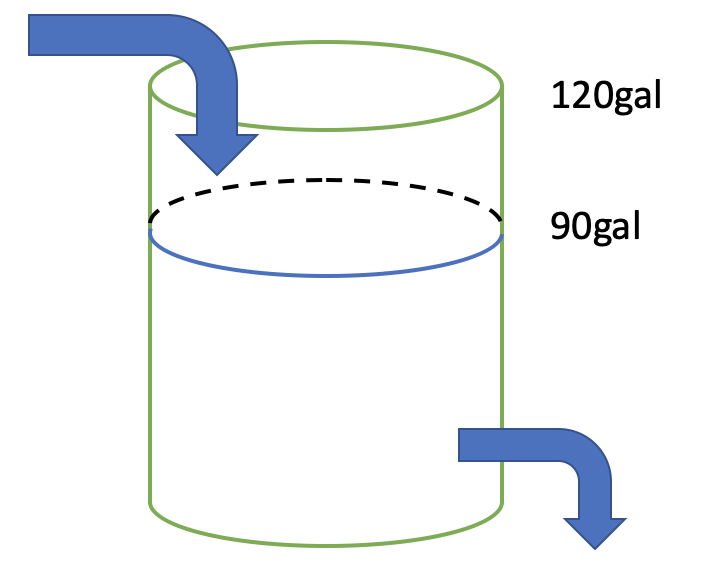
\includegraphics[width=5cm]{week2_wed_first}
\caption{First}
\end{figure}
Set $y(t)=$ the amount of salt at time $t$,\\ $V(t)=$the amount of brine at time $t$= 90 +$t$(gal)(t:minute)\\
\[\begin{aligned}y^\prime(t)&=2\text{kg/gal}\cdotp4\text{gal/min}-\frac{y(t)}{V(t)}\text{kg/gal}\cdotp3\text{gal/min}\\
&=8\text{kg/min}-3\frac{y(t)}{V(t)}\text{kg/min}
\end{aligned}
\]
\[y^\prime=8-3\frac{y}{90+t}
\]
\[y^\prime+\frac{3}{90+t}y=8
\]
By intergrating factor,
\[(e^{\int\frac{3}{90+t}\diff t}\cdotp y)^\prime=8e^{\int\frac{3}{90+t}\diff t}
\]
Try to simplify $e^{\int\frac{3}{90+t}\diff t}$;
\[\begin{aligned}\int\frac{3}{90+t}\diff t&=3ln|90+t|+\tilde{c}\\&=3ln(90+t)+\tilde{c}\end{aligned}
\]
Then,
\[e^{\int\frac{3}{90+t}\diff t}=(90+t)^3\cdotp c
\]
Integrate both sides,
\[(90+t)^3\cdotp c\cdotp y=8\int(90+t)^3\cdotp c\diff t
\]
\[(90+t)^3y=2\cdotp(90+t)^4+C
\]
\[y=2(90+t)+\frac{c}{(90+t)^3}
\]
\[y(0)=90=180+\frac{c}{90^3}\quad\Rightarrow\quad c=-90^4
\]
\[y=2(90+t)-\frac{90^4}{(90+t)^3}
\]
At $t=30$ the tank is full \& $y(30)=240-\frac{90^3}{120^3}\cdotp90$
\end{example}

\begin{example}[Persuit problem]
In a naval excercise, a distroyler $D$ is hunting a submarine $S$. Suppose $D$ at $(9,0)$ detects $S$ at $(0,0)$ \& at the same time $S$ detects $D$. Assuming that $S$ will dive immediately \& depart at full speed, $15$mile/hr in a straight course of unknown direction. What path should the destroyer $D$ follows to be certain of passing directly over the submarine $S$. If the speed of $D$ is $30$mile/hr at all time of the pursuit?
\begin{figure}[H]
\centering
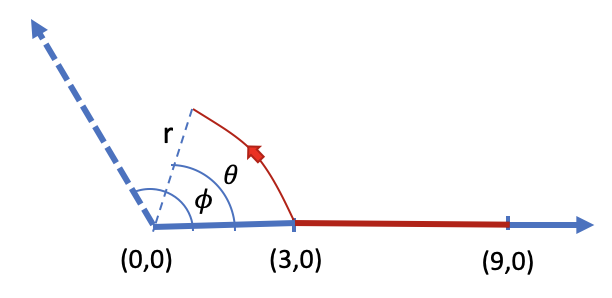
\includegraphics[width=8cm]{week2_wed_sec}
\caption{The path of destroyler in red.}
\end{figure}
Distance $D$ has travelled=$6+\int_0^\phi\sqrt{(r(\theta))^2+(r^\prime(\theta))^2}\diff\theta$.\\
Distance $S$ has travelled=$r(\phi)$.\\
For the speed of $D$ is twice than that of $S$, with the same period of time:
\[6+\int_0^\phi\sqrt{(r(\theta))^2+(r^\prime(\theta))^2}\diff\theta=2r(\phi)
\]
This isn't a form that can be dealt with. Differentiate both side,
\[\sqrt{(r(\phi))^2+(r^\prime(\phi))^2}=2r^\prime(\phi)
\]
\[(r(\phi))^2+(r^\prime(\phi))^2=4(r^\prime(\phi))^2
\]
\[r^\prime(\phi)=\pm\frac{1}{\sqrt{3}}r(\phi)
\]
W.L.O.G pick plus sign $\frac{r^\prime}{r}=\frac{1}{\sqrt{3}}$
\[lnr=\frac{1}{\sqrt{3}}\phi+\tilde{c}
\]
\[r=e^{\frac{\phi}{\sqrt{3}}}\cdotp c
\]
\[r(0)=3=c
\]
\[r(\phi)=3e^{\frac{\phi}{\sqrt{3}}}
\]
Given the direction $S$ take $\phi$, if $D$ want to be above it, they would reach each other at $(\phi,3e^{\frac{\phi}{\sqrt{3}}})$. This implies that if $D$ follows the path of 
$r(\theta)=3e^{\frac{\theta}{\sqrt{3}}}$, $D$ can catch $S$ whichever direction $S$ take.
\end{example}
\begin{remark}
There is a link about basic idea of how to compute the length of a curve:
\href{http://tutorial.math.lamar.edu/Classes/CalcII/ArcLength.aspx}{http://tutorial.math.lamar.edu/Classes/CalcII/ArcLength.aspx}. Check it if you are interested.
\end{remark}
\paragraph{Orthoganal trajectories} Given a family of curve $f(x,y,c)=0$. To find its orthoganal trajectories, the slope of the graph is needed. Differentiate $F$ by $x$;
\[F_x+F_yy_x=0
\]
Slope is $y_x=-\frac{F_x}{F_y}$. Then the slope of the graph that is orthoganal to the original one is \[y_x=\frac{F_y}{F_x}=\frac{\frac{\partial F}{\partial y}(x,y,c)}{\frac{\partial F}{\partial x}(x,y,c)}\]
\begin{example}
$y=cx^2$ $c$:parameter. To find another family of curves which is orthoganal to $y=cx^2$ whenever they intersect with each other.\\
$y=cx^2$, $\frac{\diff f}{\diff x}=2cx$ O.T. $\rightarrow \frac{\diff f}{\diff x}=\frac{-1}{2cx}=\frac{-1}{2\frac{y}{x^2}x}=-\frac{x}{2y}$ ( A separable equation)\\
$2y\diff y+x\diff x=0\quad\rightarrow\quad y^2+\frac{1}{2}x^2=c$
\end{example}



\backmatter

\latexprintindex

\end{document} 
